\documentclass[11pt]{jreport}
\usepackage{wuse_thesis}
\usepackage{indentfirst}
\usepackage{listings}
\usepackage{tabularx}
\usepackage{fancyvrb}
\usepackage{xurl}
\usepackage{cite}
\usepackage[dvipdfmx]{graphicx}
\usepackage{latexsym}
\usepackage[T1]{fontenc}
\usepackage{lmodern}
\usepackage{textcomp}
\usepackage{latexsym}
\usepackage{url}
\usepackage{longtable}
\usepackage{multirow}
\usepackage{float}
%\usepackage{color}
\usepackage{xcolor}
\usepackage{colortbl}
%\usepackage[noadjust]{cite}
\usepackage{url}	% \url{}コマンド用.URLを表示する際に便利
\usepackage{amsmath}
%\usepackage{graphicx}  % ←graphicx.styを用いてEPSを取り込む場合有効にする
			% 他のパッケージ・スタイルを使う場合には適宜追加

\newcommand{\todo}[1]{\colorbox{yellow}{{\bf TODO}:}{\color{red} {\textbf{[#1]}}}}
\newcommand{\change}[1]{\colorbox{green}{{\bf CHANGE}:}{\color{blue} {\textbf{[#1]}}}}
\newcommand{\new}[1]{\colorbox{cyan}{{\bf NEW}:}{\color{black} {\textbf{[#1]}}}}
\newcommand{\rqone}{開発状況の学習有無によって検証/導入予測モデルの予測性能はリリースまでの期間内でどのように変化するか?}
\newcommand{\rqtwo}{リリースまでの期間内で検証者の検証判断/導入判断はどのように変化するか?}

%%%%%%%%%%%%%%%%%%%%%%%%%%%%%%%%%%%%%%%%%%%%%%%%%%%%%%%%%%%%%%%%%%%%%%%%

%%
%% 主に表紙を作成するための情報
%%

%%  タイトル(修論の場合は英語表記も指定)
\title{リリースまでの期間に応じて優先的に検証/導入\\されるコードレビューチケットの特定}
\etitle{Prioritized Identification of Reviewed or Merged\\Review Tickets for Each Period before Release}

%%  著者名(修論の場合は英語表記も指定)
\author{上中 瑞稀}
\eauthor{Mizuki Uenaka}

%% 卒業論文・修士論文(以下のどちらかを選択)
%\bachelar	% 卒業論文(4年生用)
\master  	% 修士論文(M2用)

%%  学科・クラスタ
%\department{システム工}
\department{システム知能}

%%  学生番号
\studentid{S2320020}

%%  卒業年度
\gyear{2024}		% 提出年が2022年なら,2021年度

%%  論文提出日
\date{2025年2月}	% 修士の場合は月(2021年2月)までとし,英語表記も指定
\edate{February 2024}	% 修士の場合,こちら(英語表記)も有効化

%%%%%%%%%%%%%%%%%%%%%%%%%%%%%%%%%%%%%%%%%%%%%%%%%%%%%%%%%%%%%%%%%%%%%%%%

\begin{document}

\maketitle

%%
%%  概要
%%
\begin{abstract}
オープンソースソフトウェア (OSS) 開発において,変更提案されたソースコードの可読性や欠陥の有無を評価するコードレビューは,ソフトウェアの品質維持のために重要な役割を担っている.しかし,コードレビューはソフトウェア開発プロセスの一連の作業において,時間,作業量ともに高いコストを要する作業であるため,昨今ではオンラインコードレビューサービスを導入することで,コードレビュー作業の効率化を図るプロジェクトが増加している.オンラインコードレビューサービスを導入するOSS開発では,日々多くのコードレビューを依頼するコードレビューチケットが提出され,検証者は優先的にコードレビューするチケットを選択する.

従来研究では,チケット報告時に得られる特徴に基づき,検証者らが優先的に検証するチケットを特定する手法を提案しており,報告時期によって優先順位の変動が小さい変更内容に関するチケットに対して有用な手法となっている.
一方で,検証する優先順位が日々変動するチケットも存在する.Kononenkoらは,開発者へのインタビューにおいて,直近のリリースに導入するチケットの優先順位はリリースまでの期間によって異なることを明らかにしている.また,様々な従来研究において,ドメインシフト(学習データとテストデータの分布が異なることで予測性能が低下する)問題に対応した予測モデルが構築されている.ソフトウェア開発においても,優先的に検証/導入されるチケットがリリースまでの期間などの開発状況によって異なるドメインシフト問題が発生し,優先的に検証/導入されるチケットの予測性能が低下することが従来研究に基づき示唆される.本研究の事前分析として,リリースまでの期間を3期間(前期,中期,後期)に分割し,それぞれの期間で優先的に検証/導入されたコードレビューチケットの特徴量を分析した結果,複数プロジェクトでリリースまでの期間に応じて優先的に検証/導入されるコードレビューチケットの特徴量に違いがあることを明らかにした.
このような結果から,従来手法はリリースまでの期間などの開発状況に応じて優先度が日々変動するチケットの優先順位の決定には適していないと考えられる.
%オンラインコードレビューサービスを導入するOSS開発では,日々多くのコードレビューを依頼するコードレビューチケットが提出され,検証者は優先的にコードレビューするチケットを選択する.従来研究では,チケット提出時に得られる特徴に基づき優先順位づけする手法が提案されているが,コードレビューするチケットの優先順位は日々変動する.本研究では,直近のリリースまでの期間に応じて検証/導入されるコードレビューチケットの特徴の違いを分析する.また,リリースまでの期間別に優先的に検証/導入されるコードレビューチケットを予測する.ケーススタディとして,OpenStackプロジェクトを対象に分析した結果,リリースまでの期間に応じて検証/導入されるチケットの特徴には違いがあることを明らかにした.また,優先的に検証/導入されるコードレビューチケットを予測した結果,優先的に検証/導入する必要のないチケットの検出では提案手法の有用性が示された.

\end{abstract}

%%  目次
\tableofcontents

%%  図目次 (図目次をいれたければ以下のコメントをはずす)
%\listoffigures

%%  表目次 (表目次をいれたければ以下のコメントをはずす)
%\listoftables

\newpage
\pagenumbering{arabic}	% 以降のページ番号を算用数字に

%%%%%%%%%%%%%%%%%%%%%%%%%%%%%%%%%%%%%%%%%%%%%%%%%%%%%%%%%%%%%%%%%%%%%%%%

%%
%%  本文はここから
%%

%%%%%%%%%%%%%%%%%%%%%%
\chapter{はじめに}
%%%%%%%%%%%%%%%%%%%%%%

オープンソースソフトウェア (OSS : Open Source Software) は,ソースコードが無償で公開されているソフトウェアであり,利用,拡張,修正,再配布といった行為を誰でも行うことができる.OSS開発において,変更提案されたソースコードの可読性や欠陥の有無を開発者が評価するコードレビューの作業は,ソフトウェアの品質維持のために重要な役割を担っている~\cite{quality1}\cite{quality2}.特にOSSにおけるコードレビューでは,複数人の開発者(検証者)がソースコードを検証し,ソースコードを実装した開発者(実装者)と共にソースコード変更の妥当性について合意形成を図り,必要に応じて修正を繰り返す.

コードレビューはソフトウェア開発プロセスの一連の作業において,時間,作業量ともに高いコストを要する作業である\cite{cost}.そこで,昨今ではGitHub,Gerrit,Review Boardなどのオンラインコードレビューサービスを利用した方式(モダンコードレビュー\cite{quality1})を導入することで,コードレビュー作業の効率化を図るプロジェクトが増加している.モダンコードレビューでは,オンラインコードレビューサービスによってソースコードの変更提案をコードレビューチケット(チケット)として保存・管理することで,ソースコードの変更履歴やコードレビューの議論を一元的に記録し,過去のレビュー内容を参照しながら開発の品質向上や知識共有を促進する.OSS開発プロジェクトでは,日々膨大なソースコードの変更提案が報告されており,検証者は変更提案の内容や緊急性から日々変動する各チケットの優先度を見積もり,優先的に検証するチケットを選択している\cite{integrator}.
%検証者は変更提案の内容や緊急性を考慮しながら優先的に検証するチケットを選択している\cite{integrator}.

従来研究では,チケット報告時に得られる特徴(変更行数や変更ファイル数など)に基づき,検証者らが優先的に検証するチケットを機械学習アルゴリズムを用いて特定する手法を提案している\cite{prioritizer}\cite{review_prioritize_pineapple}.ソフトウェア利用者に悪影響を与えるセキュリティ関連のソースコード変更は,報告時期によって優先順位の変動が小さい変更内容に関するチケットであり,このようなチケットに対して従来研究の手法は有用である.
一方で,検証する優先順位が日々変動するチケットも存在する.Kononenkoらは,開発者へのインタビューにおいて,直近のリリースに導入するチケットの優先順位はリリースまでの期間によって異なることを明らかにしている\cite{release_merge}.また,様々な従来研究において,ドメインシフト(学習データとテストデータの分布が異なることで予測性能が低下する)問題に対応した予測モデルが構築されている\cite{domain1}\cite{domain2}.ソフトウェア開発においても,優先的に検証/導入されるチケットがリリースまでの期間などの開発状況によって異なるドメインシフト問題が発生し,優先的に検証/導入されるチケットの予測性能が低下することが従来研究\cite{release_merge}に基づき示唆される.本研究の事前分析として,リリースまでの期間を3期間(前期,中期,後期)に分割し,それぞれの期間で優先的に検証/導入されたコードレビューチケットの特徴量を分析した結果,複数プロジェクトでリリースまでの期間に応じて優先的に検証/導入されるコードレビューチケットの特徴量に違いがあることを明らかにした.
このような結果から,従来手法はリリースまでの期間などの開発状況に応じて優先度が日々変動するチケットの優先順位の決定には適していないと考えられる.

% 本研究では,開発状況を説明変数として学習することで優先度が日々変動するチケットに対応した予測モデルと対応していない予測モデルの予測性能を比較し,両モデルの予測結果から予測対象となったチケットを分類することで,各分類のチケット群に共通する特徴を分析する.本研究では,コードレビューツールGerritを使用するクラウド基盤ソフトウェアOpenStackの6つのコアコンポーネントプロジェクトのチケットデータをケーススタディとして2つのリサーチクエスチョン (RQ) を検証する.

本研究では,開発状況を説明変数として学習することで優先度が日々変動するチケットに対応した予測モデルと対応していない予測モデルの予測性能を比較し,両モデルの予測結果の中で正例および負例の網羅率を分析することで,検証者の検証判断/導入判断の変化を考察する.本研究では,コードレビューツールGerritを使用するクラウド基盤ソフトウェアOpenStackの6つのコアコンポーネントプロジェクトのチケットデータをケーススタディとして2つのリサーチクエスチョン (RQ) を検証する.

\noindent\textbf{RQ1: \rqone}\\
RQ1では,従来研究\cite{prioritizer}で提案されているチケットおよびチケット実装者の特徴(7種類)と従来研究\cite{release_merge}\cite{review1}の知見から有用と示唆される実装者や変更内容の特徴(5種類)を説明変数とするモデルをベースラインモデル,さらにベースラインモデルで用いた12種類の説明変数に従来研究に基づき開発状況の特徴(3種類)を追加するモデルを提案モデルとして2種類のモデルを構築する.従来研究\cite{prioritizer}では各予測結果の予測性能の平均を算出する手法が採用されており,リリースまでの期間内で予測性能がどのように変化するかについては明らかにされていないため,ベースラインモデルにおける優先的に検証/導入されるチケットの予測性能を1日ごとに算出することで,リリースまでの期間内においてモデルの予測性能がどのように変化するかを明らかにする.また,2種類のモデルにおけるチケットの予測性能を比較することで,開発状況の学習有無による予測性能の変化を明らかにする.

\noindent\textbf{RQ2: \rqtwo}\\
RQ2では,RQ1の予測結果を元に,両モデルの正例および負例の網羅率を比較し,提案モデルの網羅率がベースラインモデルの網羅率より高くなる期間を明らかにすることで,開発状況によって検証者の検証判断/導入判断が一部のチケットで変化する期間および判断の変化を考察する.

% \noindent\textbf{RQ2: \rqtwo}\\
% RQ2では,RQ1の予測結果を元に,リリース期間全体を通して常に優先されるチケットや常に優先されないチケット,リリースまでの期間内で優先度が変化するチケットの特徴を分析することで,リリースまでの期間内で優先度が変化するチケットと変化しないチケットにはそれぞれどのような共通の特徴があるかを明らかにする.
%また,データセットとして利用しているプロジェクトの検証者にアンケート調査を行うことで,分析結果を考察する.

以降,本論文では,\ref{sec:intro}章でOSS開発におけるコードレビュープロセスと従来研究について述べる.その後,\ref{sec:pre_analysis}章で事前分析の分析手法および結果を述べる.そして,\ref{sec:analysis_method}章でRQ1,RQ2の分析手法を述べ,\ref{sec:rq1}章でRQ1,\ref{sec:rq2}章でRQ2の結果や考察を述べる.そして,\ref{sec:disc}章で妥当性の脅威について述べ,\ref{sec:fig-tab-exp}章でまとめる.

%%%%%%%%%%%%%%%%%%%%%%
\chapter{ソフトウェア開発におけるコードレビュープロセス}\label{sec:intro}
%%%%%%%%%%%%%%%%%%%%%%

\section{コードレビュープロセス}
図\ref{fig:codereviewprocess}はコードレビュー作業の一連の流れを説明する概略図を示す.検証者は,実装者が報告したコードレビューチケットのソースコードに対してコードレビューを行うことで,ソースコードの可読性やバグの混入有無等を評価する.コードレビュープロセスでは,複数人の検証者が行ったコードレビューの結果に基づいて,変更提案に対する導入判断(導入,却下,修正要求)を決定する.導入判断のうち,導入はコードレビューチケットのソースコードをリポジトリに導入し,却下はソースコードを導入することなくコードレビューチケットを閉じる.また修正要求は,コードレビューチケットを報告した実装者に,コードレビューに基づいたソースコードの改修を依頼する.ソフトウェア開発では,このようなコードレビュープロセスを設けることで,ソフトウェアの品質を維持しつつ,不具合修正やさらなる機能拡張を効率的に行っている.

コードレビューはソフトウェア開発に多大な貢献をもたらす一方で,膨大なコストがかかる作業でもある.1つのコードレビューチケットの確認に数日から数ヶ月の期間を要することもあり,1週間で平均6時間程度をコードレビューに費やすプロジェクトも多い\cite{review2}.特に,大規模なオープンソースソフトウェア (OSS) 開発では,膨大なチケットを受け付けるため,検証者は変更提案の内容や緊急性を考慮して,優先的に検証するチケットを選択している\cite{integrator}.

%-----------------------
\begin{figure}[h]
\begin{center}
\scalebox{0.9}{
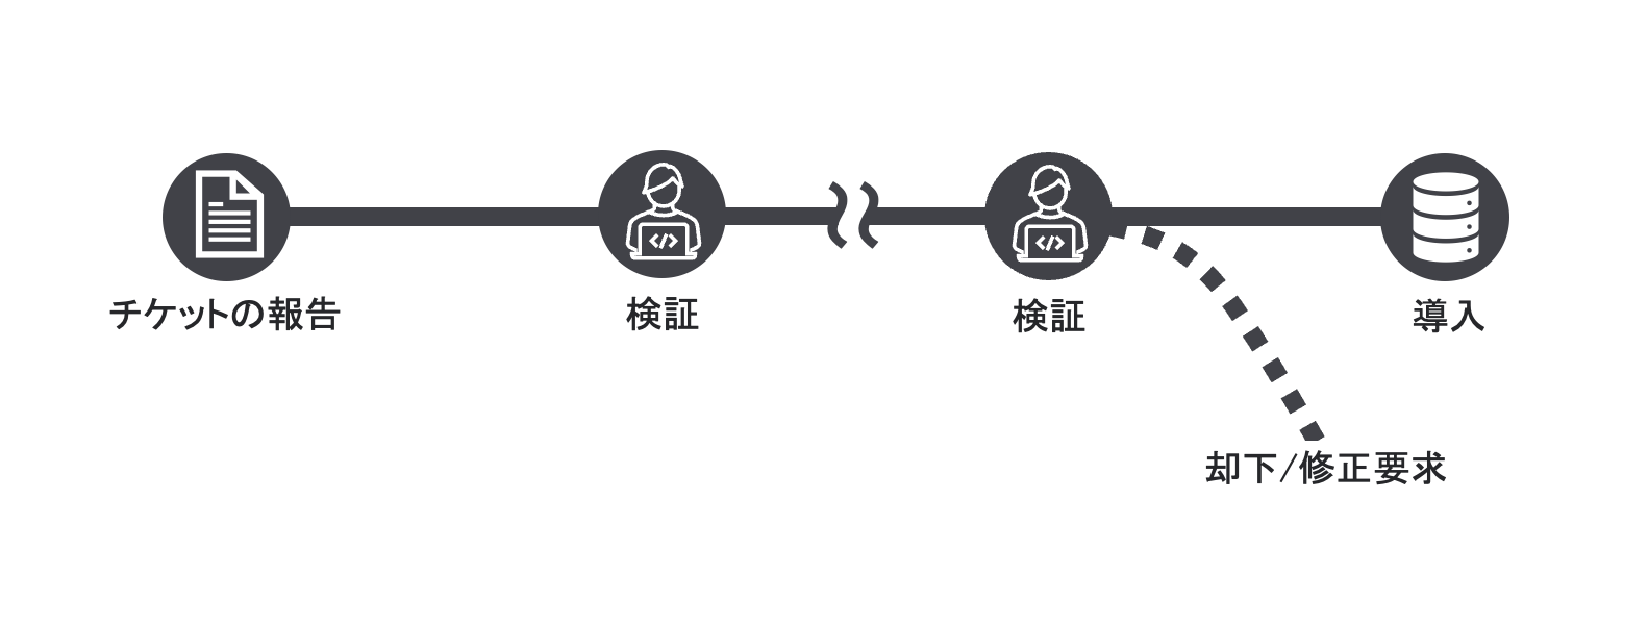
\includegraphics[width=1.0\linewidth]{Uenaka_fig/code_review_process.pdf}
}
\caption{コードレビュープロセス}
\label{fig:codereviewprocess}
\end{center}
\end{figure}
%-----------------------

\section{関連研究}
\subsection{コードレビューチケットの優先順位付け}
Veen\cite{prioritizer}らは,OSS開発を対象にコードレビューの優先順位付け手法を提案している.従来研究では,機械学習アルゴリズムを用いて,変更内容や作成者の特徴などの14種類の特徴を説明変数とし,コードレビューチケットに翌日までに検証結果が投稿されるか否かを予測する手法を提案している.当該研究ではリリースまでの期間などの開発状況によって日々優先順位が変動するような変更提案のチケットに対して誤った優先順位を算出することが示唆される.そのため,本研究ではリリースまでの期間などの開発状況を説明変数に用いた予測モデルを構築し,開発状況を説明変数に用いていない予測モデルと予測性能を比較する.また,当該研究では全ての予測における予測性能の平均を取ることで予測性能を算出しているため,リリースまでの期間内で予測性能がどのように変化するかについては明らかにされていない.そのため,本研究ではリリースまでの期間内におけるモデルの予測性能を1日ごとに算出することで,モデルの予測性能がどのように変化するかを明らかにする.

\subsection{開発者の貢献量がチケットの検証/導入判断にもたらす影響}
Bosu\cite{review1}らは,OSS開発における開発者の地位(例えば,コミッター)がチケットの導入に影響するのか否かを明らかにするために,OSS開発に積極的に貢献する開発者と消極的な開発者がそれぞれ作成したソースコードのレビュープロセスの違いを調査した.8つのOSSプロジェクトから導入もしくは却下と判断されたチケットのコードレビューデータを調査した結果,積極的に貢献する開発者のチケットほど,導入もしくは却下までの時間が短く,導入される確率が高いことが明らかとなった.そのため本研究では,実装者の貢献量を捉えるため,従来研究\cite{prioritizer}の説明変数である導入実績(実装者が過去に提案したチケットの導入率)だけでなく,報告実績(実装者が過去に提案したチケット数),直近導入実績(実装者が過去に提案したチケットの3ヶ月以内の導入率),直近報告実績(実装者が過去3ヶ月以内に提案したチケット数)を説明変数に加え,優先的に検証/導入されるチケットを予測する.

\subsection{コードレビューにかかる時間および導入判断に影響を与える要因}
Kononenko\cite{release_merge}らは,コードレビューにかかる時間や導入判断に影響を与える要因を明らかにするためにコードレビューチケットを調査し,定性的分析として検証者へのインタビューを行った.検証者へのインタビュー内容を調査した結果,一部の検証者の意見から,レビューにかかる時間は変更内容(バグ修正,リファクタリング等)によって異なることが明らかとなった.そのため,本研究では変更内容によって検証判断が異なると考え,従来研究\cite{bug}\cite{refactoring}において定義された正規表現をチケットのタイトルと概要に適用することで得られる特徴量を,バグ修正確信度とリファクタリングとして説明変数に加え,優先的に検証/導入されるチケットを予測する.
また,導入判断はリリースまでの期間によって異なることが明らかとなった.本研究ではこの知見をキーアイデアとし,リリースまでの期間に焦点を当てた研究を実施する.
%また,リリースまでの期間だけでなく,プロジェクトに報告されているチケット数や検証者がコードレビューできる行数を含めた開発における外的要因をまとめて開発状況と定義し,開発状況に焦点を当てた研究を行う.

%Kononenko\cite{release_merge}らは,コードレビューにかかる時間および導入判断に影響を与える要因を明らかにするためにコードレビューチケットを調査した.定性的分析として検証者へのインタビューを行った結果,レビューにかかる時間は変更内容(バグ修正,リファクタリング等)によって異なることが明らかとなった.そのため,本研究では変更内容によって検証判断が異なると考え,従来研究\cite{bug}\cite{refactoring}において利用されていた
%チケットのタイトルと概要に含まれる単語に基づき,バグ修正,リファクタリング,またはその他に分類し,バグ修正確信度とリファクタリングを説明変数に加え,優先的に検証/導入されるチケットを予測する.

\section{Research Questions}
本研究では,2つのResearch Questionsを検証することで,開発状況が予測性能に与える影響やリリースまでの期間内における検証者の判断の変化を明らかにする.
% 本研究では,2つのResearch Questionsを検証することで,開発状況が予測性能に与える影響やリリースまでの期間内において優先度が変化する/しないチケットに共通する特徴を明らかにする.

%-----------------------
\begin{itemize}
  \item \textbf{RQ1: \rqone}
  \item \textbf{RQ2: \rqtwo}
\end{itemize}
%-----------------------

本研究では,チケットおよびチケット実装者の特徴のみを説明変数とするモデル(ベースラインモデル)と開発状況の特徴を追加で説明変数とするモデル(提案モデル)の2種類を構築し,優先的に検証/導入されるコードレビューチケットを予測する.RQ1では,リリースまでの期間内におけるベースラインモデルの予測性能の変化および両モデルの予測性能の違いを分析する.
RQ2では,両モデルの予測結果を元に,両モデルの正例および負例の網羅率を比較し,提案モデルの網羅率がベースラインモデルの網羅率より高くなる期間を分析することで,開発状況によって検証者の検証判断/導入判断が一部のチケットで変化する期間および判断の変化を考察する.


% 本研究では,チケットおよびチケット実装者の特徴のみを説明変数とするモデル(ベースラインモデル)と開発状況の特徴を追加で説明変数とするモデル(提案モデル)の2種類を構築し,優先的に検証/導入されるコードレビューチケットを予測する.RQ1では,リリースまでの期間内におけるベースラインモデルの予測性能の変化および両モデルの予測性能の違いを分析する.RQ2では,両モデルの予測結果を比較し,分析対象となったチケットを分類することでリリースまでの期間内で優先度が変化するチケットと変化しないチケットにはそれぞれどのような共通の特徴があるかについての分析を行う.


%また,データセットとして利用しているプロジェクトの検証者にアンケート調査を行うことで,分析結果を考察する.


%\section{本研究の動機}
%従来研究\cite{prioritizer}は,優先順位の変動が小さいコードレビューチケットの特定には有用である.しかし,提出されるチケット数に対して検証可能な開発者数のような開発リソースが少ない場合,検証/導入可能なチケット数に限りがあるため,リリースまでの期間に検証の優先順位が変化するチケットの特定には適していない.特に,ラピッドリリースを導入しているプロジェクトでは検証を次のリリースに延期することも少なくない.

%そこで,本研究では,事前分析としてリリースまでの期間に着目し,リリースまでの期間別に検証/導入されるコードレビューチケットの特徴を分析する.また,RQ1では,開発者やチケットの特徴のみを特徴量として用いたモデルと開発者やチケットの特徴だけでなく追加で開発状況を特徴量として用いたモデルの2種類を構築し,優先的に検証/導入されるコードレビューチケットの予測性能を比較する.RQ2では,RQ1の結果の考察として,リリースまでの期間内で優先度が変化するチケットと変化しないチケットにはどのような違いがあるかについての分析および目視を行う.また,データセットとして利用しているプロジェクトの検証者にアンケート調査を行うことで,分析結果を考察する.


%%%%%%%%%%%%%%%%%%%%%%
\chapter{事前分析:リリースまでの期間に応じた優先されるチケットの変化の有無の調査}\label{sec:pre_analysis}
%%%%%%%%%%%%%%%%%%%%%%

\section{概要}
事前分析では,優先的に検証/導入されるコードレビューチケットの特徴量がリリースまでの期間によって異なるかを明らかにする.具体的には,図\ref{fig:labeling}に示すようにリリースまでの期間を前期,中期,後期に3分割する.そして,それぞれの期間においてチケットを検証開始済/非検証や導入済/非導入の2クラスに分類(\ref{sec:bunrui}項で後述)し,各クラスのチケット群の特徴量を計測(\ref{sec:metrics}項で後述)し,各クラスのチケット群の特徴量の有意差を算出し,各期間で比較する(\ref{sec:compare}項で後述)ことで,優先的に検証/導入されたチケットの特徴量の期間ごとの違いを分析する.
%リリースまでの期間という開発状況がチケットの検証判断/導入判断に影響を与えるのかを明らかにするために,

\section{優先されるチケットと優先されないチケットの特徴量比較}
\subsection{コードレビューチケットの分類}\label{sec:bunrui}
\textbf{(1.検証)} 本研究では各期間において,検証者からのコメントや評価が投稿されたチケットを優先的に検証されるチケットと捉え「検証開始済」に分類し,チケットの報告以降,検証者からのコメントや評価が投稿されていないチケットを優先的に検証されないチケットと捉え「非検証」に分類する.本研究では,検証されていないチケットの中で,優先的に検証を要すると判断されるチケットの時期に応じた特徴の違いを明らかにするため,検証が開始されたチケットは,次の期間以降から分析対象外とする.
図\ref{fig:labeling}のチケットを例に説明すると,対象チケットは前期に報告されているものの,前期においてまだ検証されていないため,前期では「非検証」に分類する.また,中期において検証が開始されたため,中期では「検証開始済み」に分類し,後期以降は分析対象外とする.

\textbf{(2.導入)} 本研究では各期間において,GitHubリポジトリに導入されたチケットを優先的に導入されるチケットと捉え「導入済」に分類し,チケットが報告されてからリポジトリに導入されていないチケットを優先的に導入されないチケットと捉え「非導入」に分類する.また,検証と同じく,「導入済」のチケットは,次の期間以降から分析対象外とする.
図\ref{fig:labeling}のチケットを例に説明すると,対象チケットは前期に報告されているものの,前期や中期において導入されていないため,前期や中期では「非導入」に分類する.また,後期においてリポジトリに導入されたため,後期では「導入済」に分類し,以降は分析対象外とする.

%-----------------------
\begin{figure}[h]
\begin{center}
\scalebox{1.2}{
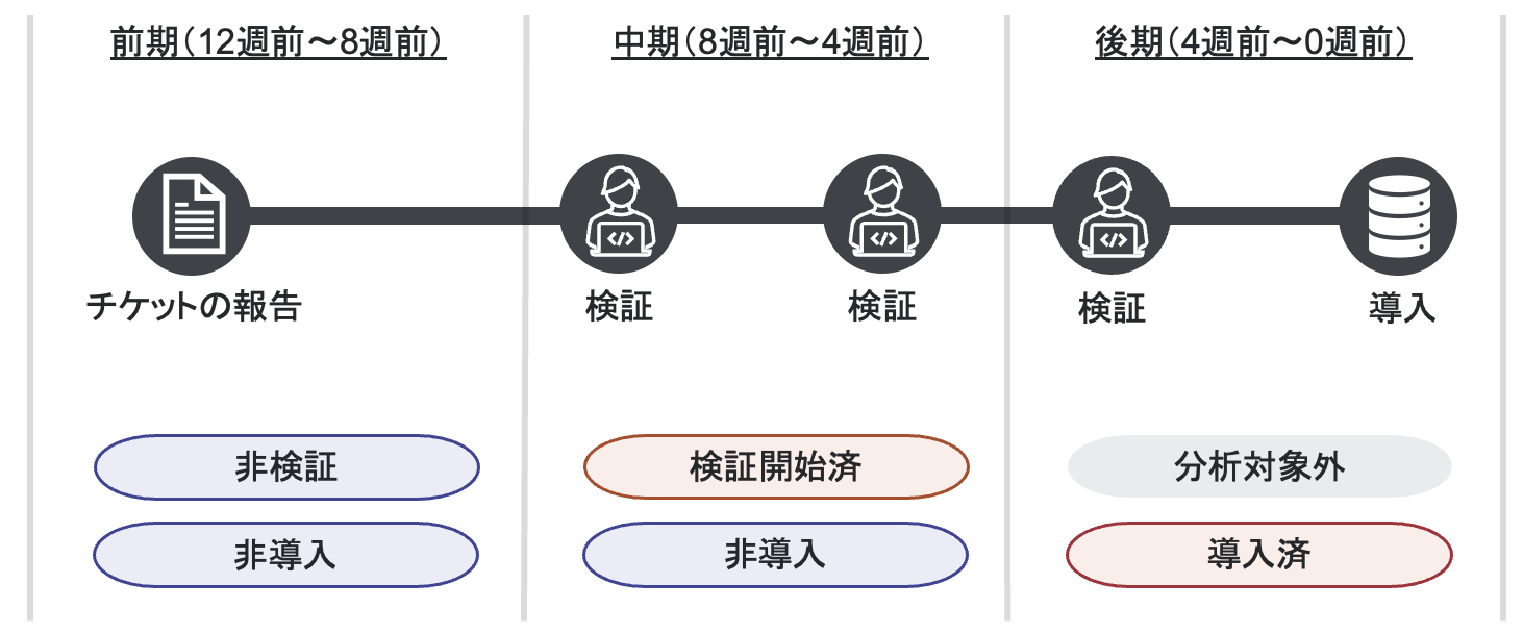
\includegraphics[width=0.8\linewidth]{Uenaka_fig/classification_method.pdf}
}
\caption{チケットの分類例}
\label{fig:labeling}
\end{center}
\end{figure}
%-----------------------


\subsection{コードレビューチケットの特徴量の計測}\label{sec:metrics}
事前分析では,\ref{sec:bunrui}項において2クラスに分類したチケットから特徴量を計測する.本分析では,時系列によって値が変化する特徴量を用いているため,同一の変更提案でもリリースまでの期間ごとに特徴量を再計測する.そのため特徴量の計測タイミングは2種類あり,期間内に報告されたチケットは報告時点の特徴量を計測し,既に報告されていたチケットは各期間の開始時点の特徴量を計測する.図\ref{fig:labeling}のチケットを例に説明すると,対象チケットは前期に報告されているため,前期では報告時点の特徴量を計測し,中期や後期では各期間の開始時点の特徴量を計測する.
具体的に事前分析で用いる特徴量について説明する.事前分析では,表\ref{table:metrics}に示す12種類の特徴量を\ref{sec:bunrui}項において2クラスに分類したチケットから計測する.12種類の特徴量は,従来研究\cite{prioritizer}において用いられていた特徴量や,従来研究\cite{release_merge}\cite{review1}の知見から有用と示唆される特徴量である.ただし,従来研究\cite{prioritizer}において用いられていた特徴量のうち,コミット数のようなGitHub特有の特徴量は計測対象外とする.
従来研究\cite{release_merge}\cite{review1}の知見から有用と示唆される特徴量のうち,バグ修正確信度は従来研究\cite{bug}において利用されていた正規表現をチケットのタイトルと概要に適用することで,チケットがバグである確度を3クラスに分類した特徴量である.
%なお,本研究では報告実績等の時系列によって値が変化する特徴量を用いているため,同一の変更提案でもリリースまでの期間ごとに再計測する.

%-----------------------
\begin{table}[h]
  \caption{事前分析に用いる12種類の特徴量}
  \label{table:metrics}
  \centering
  \vspace{0.5zh}
    \scalebox{1.08}{
  \begin{tabular}{l|l|l}
    \hline \hline
    \multicolumn{1}{c|}{特徴量}  & \multicolumn{1}{c|}{説明}  & \multicolumn{1}{c}{従来研究}  \\
    \hline
    報告実績  & 実装者が過去に報告したチケット数  & \cite{review1} \\
    直近報告実績  & 実装者が過去3ヶ月以内に報告したチケット数  & \cite{review1} \\
    導入実績  & 実装者が過去に報告したチケットの導入率  & \cite{review1},\cite{prioritizer} \\
    直近導入実績  & 実装者が過去3ヶ月以内に報告したチケットの導入率  & \cite{review1} \\
    追加行数  &  チケットで追加されている変更行数  & \cite{prioritizer},\cite{diff} \\
    削除行数  & チケットで削除されている変更行数  & \cite{prioritizer},\cite{diff}  \\
    ファイル数  & チケットで変更されているファイル数  & \cite{prioritizer} \\
    リビジョン数  & チケットの分析時点のリビジョン数  & \cite{prioritizer} \\
    経過時間  & チケットが報告されてからの経過時間  & \cite{prioritizer} \\
    テストコード含有  & 変更ファイルにテストが含まれているか  & \cite{prioritizer} \\
    バグ修正確信度  &  バグ修正の変更提案である確度  & \cite{bug},\cite{release_merge} \\
    リファクタリング  & リファクタリングの変更提案か否か  & \cite{refactoring},\cite{release_merge} \\
    \hline
  \end{tabular}
  }
\end{table}
%-----------------------

\subsection{コードレビューチケットの特徴量の比較}\label{sec:compare}
前期,中期,後期の3期間において優先的に検証/導入されるコードレビューチケットの特徴量を分析する.具体的には,各期間における検証開始済チケットと非検証チケット間や,導入済チケットと非導入チケット間の各特徴量の統計的有意差を算出する.統計検定手法として,比例尺度の特徴量に対してはマンホイットニーのU検定,名義尺度の特徴量に対してはカイ2乗検定を用いてP値を算出することで,統計的有意差の有無を明らかにする.有意差がある場合,当該期間における2クラス(検証開始済チケットと非検証チケット,もしくは導入済チケットと非導入チケット)間の特徴量に違いがあることを示す.

また,リリースまでの期間による各特徴量の有意差の違いを分析することで,リリースまでの期間によって優先的に検証/導入されるチケットの特徴量が異なるかを明らかにする.具体的には,前期では統計的有意差の無い特徴量Aに,後期では統計的有意差がある場合,特徴量Aは前期ではチケットの検証/導入判断に影響しない一方で,後期ではチケットの検証/導入判断に影響することが示唆される.つまり,リリースまでの期間によって検証/導入判断における特徴量Aの重要度が変化すると解釈する.


\section{データセット}\label{sec:dataset}
本研究では,OpenStackプロジェクトのうち,コアコンポーネント6プロジェクト(Nova,Neutron,Cinder,Keystone,Swift,Glance)を分析対象とし,各プロジェクトの変更提案の中で,立ち上げ時から2022年9月までに導入もしくは却下されたコードレビューチケットを収集した.変更提案のチケットの特徴量を計測するために,OpenStackがコードレビュー管理システムとして使用するGerrit\footnote{Gerrit: \url{https://review.opendev.org}}から,コードレビュー履歴を収集した.また各バージョンのリリース日を特定するために,Gitから各バージョンのリリース履歴を収集した.各チケットが導入されたリリースを特定するために,Gitから各プロジェクトのコミット履歴を収集し,コミットの親子関係を追跡した.

本研究では,各プロジェクトで5つのバージョンリリースに検証/導入されたコードレビューチケットの変更提案を対象とする.分析対象プロジェクトのリリース間隔が約3ヶ月であるため,特にリリース直前の3ヶ月に導入されたチケット数上位5バージョンを分析対象とすることで,「導入済」に分類されるチケットの多いバージョンを対象とした分析を行う.表\ref{table:release}は分析対象とする各プロジェクトのバージョンを示す.また,長期間に渡り放置される変更提案は,短期的な優先順位の決定には関与しないため,リリース直前の6ヶ月以内に提出されたチケットを分析対象とする.

%------------------------
\begin{table*}[h]
\centering
  \caption{プロジェクトごとの対象リリースバージョン}
  \vspace{0.5zh}
  \label{table:release}
  \scalebox{0.80}{
  \begin{tabular}{l|r|l}  \hline \hline
    プロジェクト & チケット数 & \multicolumn{1}{c}{バージョン(リリース3ヶ月以内に導入されたチケット数 )}\\ \hline 
    Nova & 39,870 & 13.0.0.0b3(529),14.0.0.0b1(475),16.0.0.0b2(451),17.0.0.0b1(410),20.0.0.0rc1(392)\\ 
    Neutron & 24,467 & 7.0.0.0b1(326),8.0.0.0b1(400),9.0.0.0b1(296),11.0.0.0b1(286),16.0.0.0b1(186)\\ 
    Cinder & 17,155 & 8.0.0.0b1(249),8.0.0.0rc1(249),9.0.0.0b2(249),11.0.0.0b2(249),12.0.0.0b2(235)\\ 
    Keystone & 10,764 & 8.0.0a0(182),9.0.0.0b3(211),10.0.0.0b2(220),11.0.0.0b1(167),15.0.0.0rc1(165)\\ 
    Swift & 8,737 & 1.9.2(180),2.4.0(154),2.7.0(117),2.17.0(105),2.27.0(101)\\ 
    Glance & 6,248 & 11.0.0a0(70),12.0.0.0b1(83),12.0.0.0b3(72),13.0.0.0b1(64),17.0.0.0b1(73)\\ \hline
  \end{tabular}
  }
\end{table*}
%------------------------

\section{リリースまでの期間に応じた優先されるチケットの変化}
事前分析では,リリースまでの期間(前期,中期,後期)に応じて,検証開始済/非検証のチケットや導入済/非導入のチケットの特徴量の間の統計的有意差を算出することで,チケットの特徴量を比較する.結果の表では,P値が0.01未満は***,0.01〜0.05は**,0.05〜0.1は*で表記する.

%--------------------
\begin{table*}[h]
\caption{検証開始済チケットと非検証チケットの特徴量の検定結果}
\label{table:review_notreview_prepare}
\centering
\vspace{0.5zh}
\scalebox{0.76}{
\begin{tabular}{l|ccc|ccc|ccc|ccc|ccc|ccc}
    \hline \hline
    \multirow{2}{*}{特徴量} & \multicolumn{3}{c|}{Nova} & \multicolumn{3}{c|}{Neutron} & \multicolumn{3}{c|}{Cinder} & \multicolumn{3}{c|}{Keystone} & \multicolumn{3}{c|}{Swift} & \multicolumn{3}{c}{Glance} \\ \cline{2-19}
    & 前 & 中 & 後 & 前 & 中 & 後 & 前 & 中 & 後 & 前 & 中 & 後 & 前 & 中 & 後 & 前 & 中 & 後 \\ \hline
    導入実績 & *** & *** & *** & *** & *** & *** &  & * & *** &  & ** & *** &  &  &  & *** & *** & *** \\
    直近導入実績 & *** & *** & *** & *** & *** & *** &  & * & *** & * &  & *** &  & *** & *** & *** & ** & *** \\
    報告実績 &  &  &  &  &   & *** & ** & *** &  & *** & *** &   &  & * & *** & ** &  &  \\
    直近報告実績 &  & ** & *** & ** &   & *** & * & ** &  & *** & *** &   & * &  & ** &  &  &  \\
    追加行数 & *** & *** & *** & *** & *** & *** & * & *** & *** & *** & *** & *** & *** & *** & *** & *** & *** & *** \\
    削除行数 & * &  &  & *** & * &  &  &  & ** &  &  &  & ** & *** &  &  &   &  \\
    ファイル数 & *** & *** & *** & *** & *** & *** &  & ** & * & *** & * & *** & *** & *** & *** & *** & *** & *** \\
    リビジョン数 & *** & *** & *** & *** & *** & *** & *** & *** & *** & *** & *** & *** & *** & *** & *** & *** & *** & *** \\
    経過時間 & *** & *** & *** & *** & *** & *** & ** & * & *** & *** & *** & *** & *** & *** & *** & *** & *** & *** \\
    テストコード含有 & *** & *** &  &  &  & ** &  &  & * & *** &   & * &  &  &  &  & * &  \\
    バグ修正確信度 & *** & *** & *** & *** & *** & *** & *** & *** & *** & ** &   & * &  &  &  & *** & ** & *** \\
    リファクタリング &  &  &  &  & * &  &  & ** & ** & ** &   &  &  &   &  &    &   &  \\ \hline
\end{tabular}}


\vspace{2mm}
\caption{導入済チケットと非導入チケットの特徴量の検定結果}
\label{table:merge_notmerge_prepare}
\centering
\vspace{0.5zh}
\scalebox{0.76}{
\begin{tabular}{l|ccc|ccc|ccc|ccc|ccc|ccc}
    \hline \hline
    \multirow{2}{*}{特徴量} & \multicolumn{3}{c|}{Nova} & \multicolumn{3}{c|}{Neutron} & \multicolumn{3}{c|}{Cinder} & \multicolumn{3}{c|}{Keystone} & \multicolumn{3}{c|}{Swift} & \multicolumn{3}{c}{Glance} \\ \cline{2-19}
    & 前 & 中 & 後 & 前 & 中 & 後 & 前 & 中 & 後 & 前 & 中 & 後 & 前 & 中 & 後 & 前 & 中 & 後 \\ \hline
    導入実績 & *** & *** & *** & *** & *** & *** & *** & *** & *** & *** & *** & *** & *** & *** & *** & *** & *** & *** \\
    直近導入実績 & * & *** & *** & *** & *** & *** & * & * & *** & *** & *** & *** & *** & ** & *** & * & ** &  \\
    報告実績 & *** & *** & *** & *** & *** & *** & *** & *** & *** & *** & *** & *** & * &  &  & *** & * &  \\
    直近報告実績 &  &  & *** &  &  & *** & ** &  & * & *** & *** & *** & *** & *** & *** &  &  &  \\
    追加行数 & *** & *** & *** & *** & *** & *** & *** & *** & *** & * & *** & *** & *** & *** & *** & * & *** & *** \\
    削除行数 &   &  &  & ** &  &   &  & ** &  &   &   &   &   &    & * &  &  & ** \\
    ファイル数 & *** &  &  & ** & * & ** &  &  &  &  &  &  & * & * &  & ** &  &  \\
    リビジョン数 &  &  & *** & * &  & *** &  &  &  &  &  &  &  & ** & * & *** &  &  \\
    経過時間 &  & *** & *** & *** & *** &  &  & ** & *** &  & ** & *** &  & *** &  & *** & * & ** \\
    テストコード含有 & *** & *** & *** & *** & *** & *** &  & *** &  & *** & *** & ** &  & * & ** & *** & ** &    \\
    バグ修正確信度 & *** & *** & *** & *** & *** & *** & *** & *** &  &  & *** & * &  & ** &  & * & ***  & *** \\
    リファクタリング & *** &   & ** &  &  &  & ** &   &   &   &   &  & * &   & ** & ** & * & * \\ \hline
\end{tabular}}
\end{table*}
%--------------------

\textbf{(検証)} 表\ref{table:review_notreview_prepare}は,各プロジェクトの前期,中期,後期における検証開始済チケットと非検証チケット間の特徴量の検定結果を示す.表\ref{table:review_notreview_prepare}の結果から,多くのプロジェクトにおいて追加行数,リビジョン数,経過時間の特徴量はいずれの期間でも検証開始済/非検証のチケット間で統計的に有意な差があることを確認した.したがって,追加行数,リビジョン数,経過時間はどの時期でもチケットの検証判断に影響することが示唆される.次に,導入実績はCinderプロジェクトやKeystoneプロジェクトにおいて,前期では統計的有意差を確認できなかったが,中期や後期それぞれでは統計的有意差を確認できた.したがって,CinderプロジェクトやKeystoneプロジェクトにおいて,導入実績は前期ではチケットの検証判断に影響しない一方で,中期や後期ではチケットの検証判断/導入判断に影響する,つまりリリースまでの期間によって検証判断における導入実績の重要度が変化することが示唆される.導入実績の他にも,報告実績,テストコード含有などの特徴量は,複数プロジェクトにおいて統計的有意差の有無が変化したため,検証判断において重要度が変化することが示唆される.
図\ref{fig:review_notreview}は,統計的有意差の有無が変化した特徴量の一例として,Cinderプロジェクトの検証開始済チケットと非検証チケットの導入実績の分布を示す.横軸はリリースまでの期間,縦軸は導入実績を表し,各期間における箱髭図は左が検証開始済チケット,右が非検証チケットにおける導入実績を表している.図\ref{fig:review_notreview}の結果から,後期における検証開始済チケットと非検証チケットをそれぞれ作成した実装者の導入実績(中央値の差)は,前期や中期に比べて大きく,後期には導入実績の高い実装者が作成したチケットが優先的に検証されていることが示唆される.したがって,リリースまでの期間に応じて検証されるチケットの特徴には違いがあることが示唆された.


%-----------------------
\begin{figure}[h]
\begin{center}
\scalebox{1.2}{
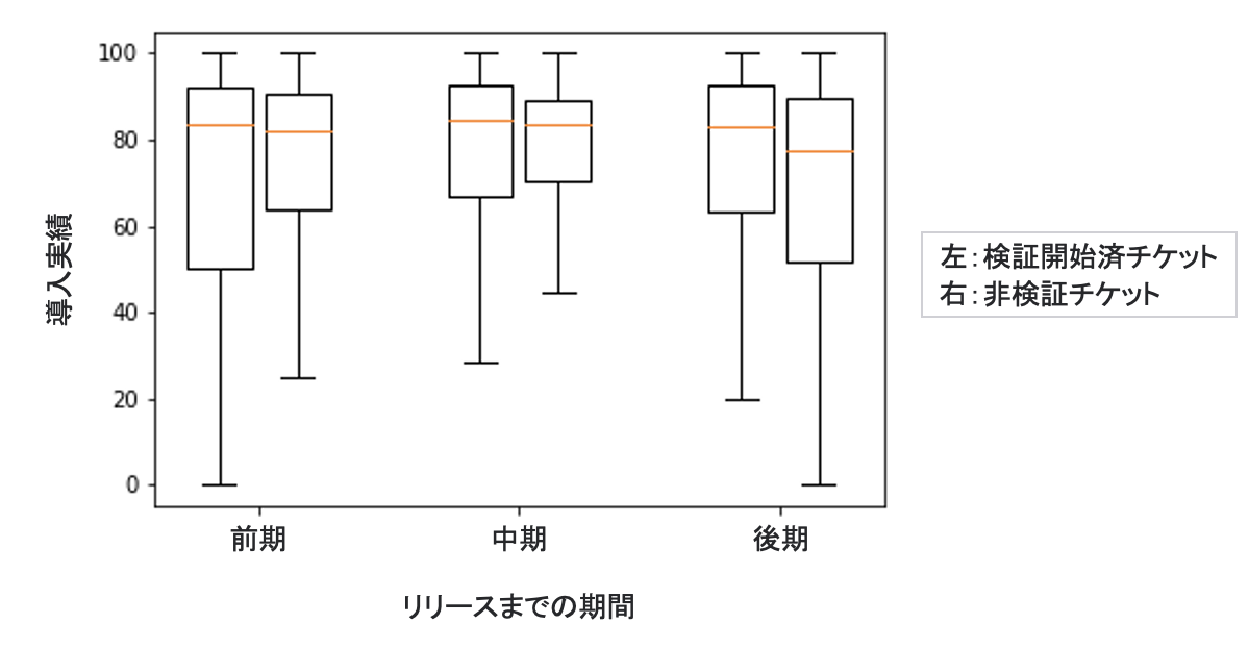
\includegraphics[width=0.8\linewidth]{Uenaka_fig/review_notreview.pdf}
}
\caption{Cinderプロジェクトにおける検証開始済/非検証のチケットの導入実績の分布}
\label{fig:review_notreview}
\end{center}
\end{figure}
%-----------------------

\textbf{(導入)} 表\ref{table:merge_notmerge_prepare}は各プロジェクトの前期,中期,後期における導入済チケットと非導入チケット間の特徴量の検定結果を示す.表\ref{table:merge_notmerge_prepare}の結果から,導入実績,追加行数の特徴量は全てのプロジェクトの全期間において,導入済/非導入のチケット間で統計的に有意な差があった.この結果から,導入実績,追加行数はどの時期でもチケットの導入判断に影響することが示唆される.
%一方,バグ修正確信度は前期や後期と比べて中期の方が統計的に有意差のあるプロジェクトが増加する.図\ref{fig:merge_notmerge}にリリースまでの期間によって有意差の変化したKeystoneプロジェクトの導入済チケットと非導入チケットのバグ修正確信度の分布を示す.バグ修正確信度は変更提案がバグ修正である確度を3値に分類した特徴量であり,図\ref{fig:merge_notmerge}では黒色で示されている提案が最もバグである確度が低く,次いで斜線,白色と図\ref{fig:merge_notmerge}の積み上げ棒グラフの下部の分類ほどバグである確度が高い.この結果から,特に中期ではバグ修正確信度の低いチケットが優先的に導入されるという結果が得られた.
%なお,後期も中期と同じような結果であるが,これは終期のバグ修正確信度にも導入済/非導入のチケット間で統計的に有意な差があったためであると考えられる.したがって,リリースまでの期間に応じて導入されるチケットの特徴には違いがあることが示唆された.
次に,経過時間はNova,Cinder,Keystoneプロジェクトにおいて,前期では統計的有意差を確認できなかったが,中期や後期それぞれでは統計的有意差を確認できた.したがって,Nova,Cinder,Keystoneプロジェクトにおいて,経過時間は前期ではチケットの導入判断に影響しない一方で,中期や後期ではチケットの導入判断に影響する,つまりリリースまでの期間によって導入判断における経過時間の重要度が変化することが示唆される.また,Neutron,Swift,Glanceプロジェクトにおいても前述の3プロジェクトとは異なったリリースまでの期間において統計的有意差の有無が変化したため,これらの3プロジェクトでもリリースまでの期間によって導入判断における経過時間の重要度が変化することが示唆される.経過時間の他にも,直近導入実績,バグ修正確信度などの特徴量は,複数プロジェクトにおいて統計的有意差の有無が変化したため,導入判断において重要度が変化することが示唆される.
図\ref{fig:merge_age}は,統計的有意差の有無が変化した特徴量の一例として,keystoneプロジェクトの導入済チケットと非導入チケットの経過時間の分布を示す.横軸はリリースまでの期間,縦軸は経過時間を表し,各期間における箱髭図は左が検証開始済チケット,右が非検証チケットにおける経過時間を表している.図\ref{fig:merge_age}の結果から,後期における導入済チケットと非導入チケットの経過時間(中央値の差)は,前期や中期に比べて大きく,後期には経過時間の短いチケットが優先的に検証されていることが示唆される.したがって,リリースまでの期間に応じて導入されるチケットの特徴には違いがあることが示唆された.

%-----------------------
\begin{figure}[h]
\begin{center}
\scalebox{1.2}{
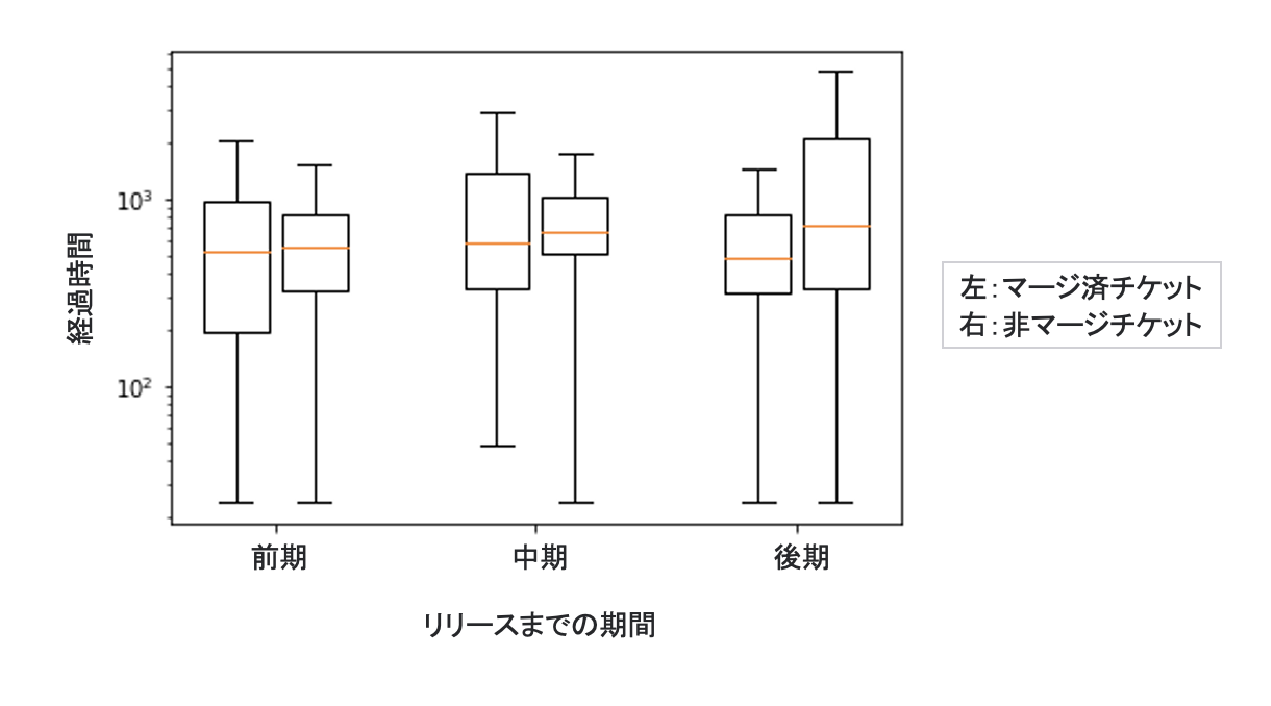
\includegraphics[width=0.8\linewidth]{Uenaka_fig/merge_age.pdf}
}
\caption{Keystoneプロジェクトにおける導入済/非導入のチケットの経過時間の分布}
\label{fig:merge_age}
\end{center}
\end{figure}
%-----------------------

\textbf{(結果のまとめ)} 事前分析の結果から,複数プロジェクトにおいて,リリースまでの期間に応じて検証/導入されるチケットの特徴には違いがあることが示唆された.


%%%%%%%%%%%%%%%%%%%%%%%%%%%%%%%%%
\chapter{開発状況に基づく優先的に検証/導入されるコードレビューチケットの特定手法とその評価}\label{sec:analysis_method}
%%%%%%%%%%%%%%%%%%%%%%%%%%%%%%%%%

RQ1では,リリースまでの期間内においてベースラインモデルの予測性能がどのように変化するか,および開発状況の学習有無によって両モデルの予測性能が異なるかを明らかにする.また,RQ2では,両モデルの正例および負例の網羅率がリリースまでの期間内でどのように異なるかを分析することで,リリースまでの期間内における検証者の検証判断/導入判断の変化を考察する.
具体的には,ウィンドウサイズを2週間とするスライディングウィンドウを定義し,1日ずつずらしながら予測モデルの学習またはテストを行い,モデルの予測性能の変化を時系列的に分析する.予測モデルとしては,\ref{sec:pre_analysis}章で用いた特徴量のみを説明変数とするモデル(ベースラインモデル)と開発状況の特徴を追加で説明変数とするモデル(提案モデル)の2種類を構築し,優先的に検証/導入されるコードレビューチケットの予測性能を比較する.また,両モデルの正例および負例の網羅率の変化を分析することで,リリースまでの期間内における検証者の検証判断/導入判断の変化を考察する.
\ref{sec:koutiku}節で予測モデルの構築方法,\ref{sec:kenshou}節で予測モデルの検証方法,\ref{sec:hyoka}節で予測モデルの評価方法,\ref{sec:seino_jikeiretsu}節で予測性能の時系列変化の分析方法,\ref{sec:ticket_tokutei}節で検証者の検証判断/導入判断の時系列変化の分析方法を述べる.



\section{予測モデルの構築}\label{sec:koutiku}

\subsection{説明変数の計測}\label{sec:setumeihensuu}
本分析では,\ref{sec:metrics}節で計測した特徴量のみを説明変数とするモデル(ベースラインモデル)の予測性能と\ref{sec:metrics}節で計測した特徴量に加えて開発状況の特徴を説明変数とするモデル(提案モデル)の2種類のモデルを構築する.提案モデルを構築するために,表\ref{table:metrics_kaihatujoukyou}に示す3つの特徴を開発状況と定義し,提案モデルの説明変数として計測する.
なお,本分析ではウィンドウサイズを2週間とするスライディングウィンドウを定義し,1日ずつずらしながら予測モデルの学習を行うため,各ウィンドウでチケットの特徴量を計測する.特徴量の計測タイミングは\ref{sec:metrics}節と概ね同様であり,ウィンドウの期間内に報告されたチケットは報告時点の特徴量を計測し,ウィンドウの期間内より以前に報告されていたチケットは各期間の開始時点の特徴量を計測する.また,本分析では報告実績等の時系列によって値が変化する特徴量を用いているため,同一の変更提案でも各ウィンドウで再度計測する.

本研究では,上記のような説明変数を学習させることで,ベースラインモデルとしてリリース期間全体を通して検証/導入されるチケットと類似した特徴を持つチケットを正しく判別できるモデルを構築し,提案モデルとしてベースラインモデルで正しく判別できるチケットだけでなく,開発状況によって検証/導入されるか否かが変化するようなチケットも正しく判別できるモデルを構築する.

%-----------------------
\begin{table}[h]
  \caption{説明変数として計測する開発状況}
  \label{table:metrics_kaihatujoukyou}
  \centering
  \vspace{0.5zh}
    \scalebox{1.08}{
  \begin{tabular}{l|l}
    \hline \hline
    \multicolumn{1}{c|}{説明変数}  & \multicolumn{1}{c}{説明}  \\
    \hline
    リリースまでの残り日数  & ウィンドウ内の最新日からリリース日までの日数 \\
    予測対象チケット数  & ウィンドウ内の予測対象であるチケット数 \\
    検証者のレビュー行数  & ウィンドウ内でレビューされた総行数 \\
    \hline
  \end{tabular}
  }
\end{table}
%-----------------------

\subsection{目的変数の計測}
\textbf{(検証予測モデル)}本分析では,検証予測モデルとして検証が開始されるか否かを目的変数としたモデルを構築する.具体的には,報告されてから初めて検証者からのコメントや評価が投稿された日を検証が開始された日と定義し,ウィンドウ内の2週間において検証が開始されたチケットを正例クラス,検証が開始されないチケットを負例クラスとして計測する.また,本分析では検証が開始されていないチケットの中で,優先的に検証を要すると判断されるチケットの予測性能を明らかにするために,ウィンドウ内の2週間より前に検証が開始されたチケットに関しては,既に優先されたチケットとみなし分類対象外とする.

\textbf{(導入予測モデル)}本分析では,導入予測モデルとして直近のリリースに導入されるか否かを目的変数としたモデルを構築する.具体的には,報告されてから初めてGitHubリポジトリに導入された日を導入された日と定義し,ウィンドウ内の2週間において導入されたチケットを正例クラス,導入されないチケットを負例クラスとして計測する.また,本分析では導入されていないチケットの中で,優先的に導入すべきであると判断されるチケットの予測性能を明らかにするために,ウィンドウ内の2週間より前に導入されたことのあるチケットに関しては,既に優先されたチケットとみなし分類対象外とする.また,OpenStackがコードレビュー管理システムとして使用しているGerritでは,一度も検証されていないチケットは導入できない仕様となっている.そのため,導入されたことのないチケットの中でも,検証が開始されていないチケットに関しては,導入されないことが確定しているチケットとみなし分類対象外とする.

\subsection{モデルの構築方法}
本分析では,検証が開始されるか否か,直近のリリースに導入されるか否かをそれぞれ目的変数とする予測モデル(検証予測モデル,導入予測モデル)を構築する.モデルの構築にあたっては,テストコード含有やリファクタリングか否かといった名義尺度の説明変数をダミー変数に変換した上で,\ref{sec:setumeihensuu}項で計測した説明変数をベースラインモデルでは12次元,提案モデルでは15次元のベクトルに変換して入力する.
検証予測モデルおよび導入予測モデルの構築には,それぞれ機械学習アルゴリズムであるRandom Forestsモデル\cite{randomforest}を用いる.しかし,本分析では目的変数が不均衡なデータを扱うため,不均衡データに対応したBalanced Random Forestモデル\footnote{imblearn.ensemble.BalancedRandomForestClassifier: \url{https://imbalanced-learn.org/stable/references/generated/imblearn.ensemble.BalancedRandomForestClassifier.html}}を用いる.



\section{予測モデルの検証}\label{sec:kenshou}
本分析では,スライディングウィンドウを用いて1日ごとにモデルの予測性能を検証する.図\ref{fig:predict_schematic}は,予測モデルの検証方法の概略図を示す.本分析では,リリースの12週間前から1日ごとに2クラス分類モデル(提案モデル,ベースラインモデル)のテストを行う.具体的には,ウィンドウサイズを2週間とするスライディングウィンドウを定義し,ウィンドウ内のチケットを用いてテストを行うことで,各テストにおいて正例クラスのチケット(検証が開始される/導入されるチケット)を一定数確保する.定義したウィンドウを1日ずつずらしながらテストを行うことで,リリースまでの期間内においてモデルの予測性能がどのように変化するかを明らかにする.また,提案モデルとベースラインモデルの予測性能を比較することで,開発状況の学習有無によってモデルの予測性能が異なるかを明らかにする.本RQでは説明の都合上,以降は各ウィンドウをウィンドウN(最もリリースから遠いウィンドウはN=71,1日ずらすごとにN$-$1し,最もリリースに近いウィンドウはN=1)と定義する.

分析対象とするデータセットには\ref{sec:dataset}節で利用したOpenStackの6つのコアコンポーネントプロジェクトから5バージョンずつを用いる.具体的には,5バージョンのうち最も直近にリリースされたバージョンをテストデータとし,残りの4バージョンを学習データとして予測モデルを検証する.

%-----------------------
\begin{figure}[t]
\begin{center}
\scalebox{1.25}{
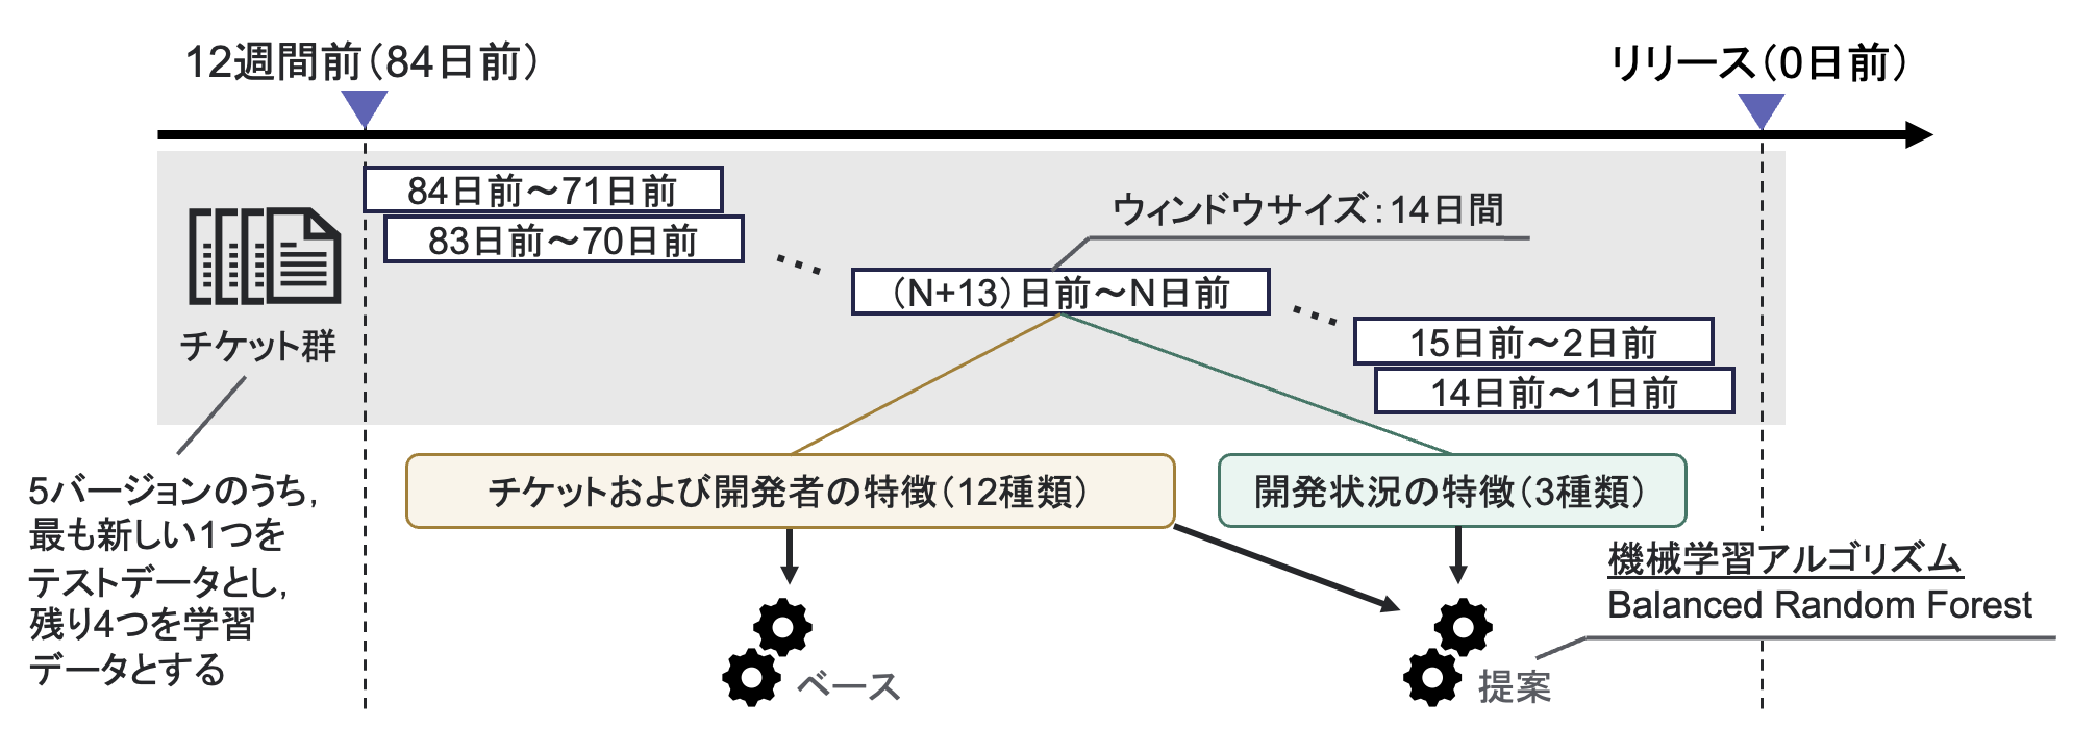
\includegraphics[width=0.8\linewidth]{Uenaka_fig/predict_schematic.pdf}
}
\caption{予測モデルの検証方法の概略図}
\label{fig:predict_schematic}
\end{center}
\end{figure}
%-----------------------



\section{予測モデルの評価}\label{sec:hyoka}
本分析では,提案モデルおよびベースラインモデルの予測性能の評価指標として適合率,再現率,F値を用い,両モデルの予測性能を比較する.評価指標の算出にあたって,両モデルの予測結果を以下の4つに分類する.

%-----------------------
\begin{itemize}
  \item \textbf{True Positive(TP):}検証が開始された/導入されたチケットに対して,検証が開始された/導入されたと正しく予測するケース
  \item \textbf{False Positive(FP):}検証が開始されない/導入されないチケットに対して,検証が開始された/導入されたと誤って予測するケース
  \item \textbf{True Negative(TN):}検証が開始されない/導入されないチケットに対して,検証が開始されない/導入されないと正しく予測するケース
  \item \textbf{False Negative(FN):}検証が開始された/導入されたチケットに対して,検証が開始されない/導入されないと誤って予測するケース
\end{itemize}
%-----------------------

以上の4つに分類した両モデルの予測結果に基づいて,以下のように適合率,再現率,F値を算出する.

適合率は,式\ref{precision}に示すように,検証が開始された/導入されたとモデルが予測したチケットの中で,検証が開始された/導入されたチケットの割合を表す.適合率は0から1の間で算出され,値が大きいほどモデルの予測性能が高いことを表す.

%-----------------------
\begin{equation}
 適合率 = \frac{TP}{TP+FP} \label{precision}
\end{equation}
%-----------------------
\vskip\baselineskip

再現率は,式\ref{recall}に示すように,検証が開始された/導入されたチケットの中で,検証が開始された/導入されたとモデルが予測したチケットの割合を表す.再現率は0から1の間で算出され,値が大きいほどモデルの予測性能が高いことを表す.

%-----------------------
\begin{equation}
 再現率 = \frac{TP}{TP+FN} \label{recall}
\end{equation}
%-----------------------
\vskip\baselineskip

F値は,式\ref{F1}に示すように,適合率と再現率の調和平均を表す.F値は0から1の間で算出され,値が大きいほどモデルの予測性能が高いことを表す.

%-----------------------
\begin{equation}
 F値 = 2 * \frac{適合率*再現率}{適合率+再現率} \label{F1}
\end{equation}
%-----------------------
\vskip\baselineskip



\section{予測性能の時系列変化}\label{sec:seino_jikeiretsu}
RQ1では,リリースまでの期間内においてベースラインモデルの予測性能がどのように変化するかを明らかにするために,各評価指標について線形回帰分析を行う.具体的には,各ウィンドウでの予測性能を$y$,各ウィンドウを$x$($x=72-N$)として回帰直線$y=a+bx$を計算することで回帰直線の傾き$b$(回帰係数)を求める.回帰係数が有意に増加または減少しているかに関してt検定を行い有意水準5\%で検定することで,各プロジェクトでのベースラインモデルの予測性能を以下の3つに分類する.

%-----------------------
\begin{itemize}
  \item \textbf{回帰係数が有意に増加する($b>0$,$P値<0.05$):}リリースが近づくにつれてベースラインモデルの予測性能が向上することを示す
  \item \textbf{回帰係数が有意に減少する($b<0$,$P値<0.05$):}リリースが近づくにつれてベースラインモデルの予測性能が低下することを示す
  \item \textbf{回帰係数が有意に増加および減少しない($P値>0.05$):}リリース時期によってベースラインモデルの予測性能が変化しないことを示す
\end{itemize}
%-----------------------



\section{検証者の検証判断/導入判断の時系列変化}\label{sec:ticket_tokutei}
RQ2では,提案モデルおよびベースラインモデルの予測結果を分析することで,開発状況によって検証者の検証判断/導入判断が一部のチケットで変化する期間および判断の変化を考察する.具体的には,ベースラインモデルの再現率(正例の網羅率)および特異度(負例の網羅率)のリリース期間内での変化を,\ref{sec:seino_jikeiretsu}節と同様に回帰係数を用いて分析する.再現率は\ref{sec:hyoka}節と同様に式\ref{recall}を用いて算出し,特異度は以下に示すように式\ref{specificity}を用いて算出する.

特異度は,式\ref{specificity}に示すように,検証が開始されない/導入されないチケットの中で,検証が開始されない/導入されないとモデルが予測したチケットの割合を表す.特異度は0から1の間で算出され,値が大きいほどモデルの負例の網羅率が高いことを表す.

%-----------------------
\begin{equation}
 特異度 = \frac{TN}{TN+FP} \label{specificity}
\end{equation}
%-----------------------
\vskip\baselineskip

% RQ2では,\ref{sec:seino_jikeiretsu}節と同様に回帰係数の算出および検定を行い,再現率および特異度の回帰係数を以下のように分類することで,各プロジェクトにおいてチケットおよびチケット実装者の特徴から正しく判別できるチケットの割合がリリースまでの期間内でどのように変化するかを明らかにする.

RQ2では,\ref{sec:seino_jikeiretsu}節と同様に回帰係数の算出および検定を行い,再現率および特異度の回帰係数を以下のように分類することで,各プロジェクトにおいてチケットおよびチケット実装者の特徴から正しく判別できるチケットの割合がリリースまでの期間内でどのように変化するかを明らかにし,検証者の検証判断/導入判断の時系列変化を考察する.

%-----------------------
\begin{itemize}
  \item \textbf{回帰係数が有意に増加する($b>0$,$P値<0.05$)}
    \begin{itemize}
      \item \textbf{再現率:}リリースが近づくにつれて,チケットおよびチケット実装者の特徴から正しく正例と判別できるチケットの割合が増加することを示す
      \item \textbf{特異度:}リリースが近づくにつれて,チケットおよびチケット実装者の特徴から正しく負例と判別できるチケットの割合が増加することを示す
    \end{itemize} 
  \item \textbf{回帰係数が有意に減少する($b<0$,$P値<0.05$)}
    \begin{itemize}
      \item \textbf{再現率:}リリースが近づくにつれて,チケットおよびチケット実装者の特徴から正しく正例と判別できるチケットの割合が減少することを示す
      \item \textbf{特異度:}リリースが近づくにつれて,チケットおよびチケット実装者の特徴から正しく負例と判別できるチケットの割合が減少することを示す
    \end{itemize} 
  \item \textbf{回帰係数が有意に増加および減少しない($P値>0.05$)}
    \begin{itemize}
      \item \textbf{再現率:}リリース期間全体を通して,チケットおよびチケット実装者の特徴から正しく正例と判別できるチケットの割合が概ね一定であることを示す
      \item \textbf{特異度:}リリース期間全体を通して,チケットおよびチケット実装者の特徴から正しく負例と判別できるチケットの割合が概ね一定であることを示す
    \end{itemize} 
\end{itemize}
%-----------------------

% 次に,提案モデルとベースラインモデルの再現率(正例の網羅率)および特異度(負例の網羅率)を比較することで,開発状況を学習したモデルにおいて正しく判別できるチケットの割合が,ベースラインモデルと比較してリリースまでの期間内でどのように増加および減少するかを明らかにする.提案モデルにおいてベースラインモデルと比較して再現率および特異度が向上する,または低下するときの解釈を以下に示す.

次に,提案モデルとベースラインモデルの再現率(正例の網羅率)および特異度(負例の網羅率)を比較し,提案モデルの網羅率がベースラインモデルの網羅率より高くなる期間を明らかにすることで,開発状況によって検証者の検証判断/導入判断が一部のチケットで変化する期間および判断の変化を明らかにする.提案モデルにおいてベースラインモデルと比較して再現率および特異度が向上するときの解釈を以下に示す.

%-----------------------
\begin{itemize}
  \item \textbf{再現率が向上する:}当該期間の一部のチケットは,開発状況によって検証者が検証を開始する/導入するようになる
  %\item \textbf{再現率が低下する:}開発状況に関わらず検証者が検証を開始する/導入するチケットが一定数存在する
  \item \textbf{特異度が向上する:}当該期間の一部のチケットは,開発状況によって検証者が検証を開始しない/導入しないようになる
  %\item \textbf{特異度が低下する:}開発状況に関わらず検証者が検証を開始しない/導入しないチケットが一定数存在する
\end{itemize}
%-----------------------

% そして,各ウィンドウにおいて予測対象となったチケットを両モデルの予測結果を用いて以下のように3種類に分類し,それぞれの分類のチケットの特徴量を分析することで,それぞれのチケットに共通する特徴を明らかにする.

% %-----------------------
% \begin{itemize}
%   \item \textbf{リリース期間全体を通して常に優先されるチケット}
%     \begin{itemize}
%       \item \textbf{(両モデルの予測結果)}提案モデル:TP,ベースラインモデル:TPまたは提案モデル:FN,ベースラインモデル:TPのチケット
%       \item 開発状況の特徴に関わらず,チケットおよびチケット実装者の特徴から正しく正例と判別できるチケットをリリース期間全体を通して常に優先されるチケットとする
%     \end{itemize} 
%   \item \textbf{リリース期間全体を通して常に優先されないチケット}
%     \begin{itemize}
%       \item \textbf{(両モデルの予測結果)}提案モデル:TN,ベースラインモデル:TNまたは提案モデル:FP,ベースラインモデル:TNのチケット
%       \item 開発状況の特徴に関わらず,チケットおよびチケット実装者の特徴から正しく負例と判別できるチケットをリリース期間全体を通して常に優先されないチケットとする
%     \end{itemize} 
%   \item \textbf{リリースまでの期間内で優先度が変化するチケット}
%     \begin{itemize}
%       \item \textbf{(両モデルの予測結果)}提案モデル:TP,ベースラインモデル:FNまたは提案モデル:TN,ベースラインモデル:FPのチケット
%       \item チケットおよびチケット実装者の特徴のみでは誤って判別する一方,開発状況の特徴を学習させることで正しく判別できるチケットをリリースまでの期間内で優先度が変化するチケットとする
%     \end{itemize} 
% \end{itemize}
% %-----------------------

% %-----------------------
% \begin{itemize}
%   \item \textbf{リリース期間全体を通して常に優先されるチケット}
%     \begin{itemize}
%       \item \textbf{(両モデルの予測結果)}提案モデル:TP,ベースラインモデル:TPまたは提案モデル:FN,ベースラインモデル:TPのチケット
%       \item 提案モデルの予測結果に関わらず,ベースラインモデルにおいて正しく正例と判別できたチケットをリリース期間全体を通して常に優先されるチケットとする
%     \end{itemize} 
%   \item \textbf{リリース期間全体を通して常に優先されないチケット}
%     \begin{itemize}
%       \item \textbf{(両モデルの予測結果)}提案モデル:TN,ベースラインモデル:TNまたは提案モデル:FP,ベースラインモデル:TNのチケット
%       \item 提案モデルの予測結果に関わらず,ベースラインモデルにおいて正しく負例と判別できたチケットをリリース期間全体を通して常に優先されないチケットとする
%     \end{itemize} 
%   \item \textbf{リリースまでの期間によって優先度が変化するチケット}
%     \begin{itemize}
%       \item \textbf{(両モデルの予測結果)}提案モデル:TP,ベースラインモデル:FNまたは提案モデル:TN,ベースラインモデル:FPのチケット
%       \item 提案モデルにおいて正しく判別できた一方,ベースラインモデルにおいて誤って判別したチケットをリリースまでの期間によって優先度が変化するチケットとする
%     \end{itemize} 
% \end{itemize}
% %-----------------------

%RQ2では,リリースまでの期間内で優先度が変化するチケットおよび変化しないチケットそれぞれに共通する特徴を明らかにする.まず,ベースラインモデルの予測結果(TP,TN)それぞれについて\ref{sec:seino_jikeiretsu}節同様に回帰直線を計算し回帰係数を求める.回帰直線を計算するにあたって,ウィンドウ内のチケット数に依存しない結果を得るために,TPはウィンドウ内の正例数で正規化した値,TNはウィンドウ内の負例数で正規化した値を各ウィンドウでの予測結果$y$として用いる.また,回帰係数が有意に増加または減少しているかに関してt検定を行い有意水準5\%で検定することで,各プロジェクトでの予測結果を以下のように分類し,リリース期間全体を通して正例(検証が開始される/導入される)および負例(検証が開始されない/導入されない)であるチケットと類似した特徴を持つチケットの割合がどのように変化するかを明らかにする.



%%%%%%%%%%%%%%%%%%%%%%%%%%%%%%%%%
\chapter{RQ1:\rqone}\label{sec:rq1}
%%%%%%%%%%%%%%%%%%%%%%%%%%%%%%%%%
RQ1では,\ref{sec:pre_analysis}章で用いた特徴量のみを説明変数とするモデル(ベースラインモデル)と開発状況の特徴を追加で説明変数とするモデル(提案モデル)の予測性能を\ref{sec:kenshou}節の検証方法および\ref{sec:hyoka}節の評価方法に基づいて1日ごとに算出する.算出した評価指標について線形回帰分析を行うことで,リリースまでの期間内においてベースラインモデルの予測性能がどのように変化するかを明らかにする.また,両モデルの予測性能を比較することで,開発状況の学習有無によるモデルの予測性能の違いを明らかにする.

\section{予測結果}
\subsection{検証予測モデル}\label{sec:rq1_kenshou}
各プロジェクトの検証予測モデルの予測結果として,図\ref{fig:review_f}はF値,図\ref{fig:review_p}は適合率,図\ref{fig:review_r}は再現率を示す.図は横軸が各ウィンドウ,縦軸が予測性能を表しており,赤の折れ線が提案モデルの予測性能,青の折れ線がベースラインモデルの予測性能を表す.また,図の左から右に向かってリリースに近いウィンドウ(最も左はウィンドウ71,最も右はウィンドウ1)での予測結果を表す.
図\ref{fig:review_f}から図\ref{fig:review_r}までの各プロジェクトにおいて,7つ以上の連続したウィンドウ(3週間以上の期間)において提案モデルの予測性能がベースラインモデルの予測性能と比べて向上した期間を赤色,ベースラインモデルの予測性能が提案モデルの予測性能と比べて低下した期間を青色で表している.予測性能の中でF値についてまとめたものを図\ref{fig:review_f1_window}に示す.
また,表\ref{table:review_seino_jikeiretsu}はベースラインモデルの予測性能の時系列変化の分析結果として,各プロジェクトの検証予測モデルにおける評価指標の回帰係数の分類を示す.表\ref{table:review_seino_jikeiretsu}において,回帰係数が有意に増加する場合は『$\nearrow$』,回帰係数が有意に減少する場合は『$\searrow$』,回帰係数が有意に増加および減少しない場合は『$\rightarrow$』で表す.

\subsubsection{知見1:検証が開始されるチケットの予測において,4プロジェクト (Nova, Neutron, Keystone, Swift) ではリリースが近づくにつれてベースラインモデルの予測性能が向上する一方,2プロジェクト (Cinder, Glance) ではリリースが近づくにつれて低下する}
本知見では,従来研究\cite{prioritizer}で明らかでなかったリリースまでの期間内での検証予測モデルの予測性能の変化を分析した.表\ref{table:review_seino_jikeiretsu}の回帰係数の分類から,ベースラインモデルのF値および適合率は4プロジェクト (Nova, Neutron, Keystone, Swift) において回帰係数が有意に増加し,2プロジェクト (Cinder, Glance) において回帰係数が有意に減少するという結果が得られた.また,ベースラインモデルの再現率は3プロジェクト (Nova, Cinder, Glance) において回帰係数が有意に増加し,3プロジェクト (Neutron, Keystone, Swift) において回帰係数が有意に増加および減少しないという結果が得られた.以下に共通の傾向を持つプロジェクトの結果をまとめる.

\textbf{ (Nova, Neutron, Keystone, Swift) }リリースが近づくにつれてベースラインモデルのF値が向上し,適合率および再現率も向上もしくは変化しなかったため,これらのプロジェクトではリリースが近づくにつれてベースラインモデルの予測性能が向上することを明らかにした.このことから,これらのプロジェクトの検証者にとって,従来研究\cite{prioritizer}のようなモデル(ベースラインモデル)はリリースが近づくにつれて有用となることが示唆されたため,これらのプロジェクトの検証者はリリースが近づくにつれて,チケットおよびチケット報告者の特徴から検証を開始するチケットを判断する傾向にあることが示唆される.

\textbf{ (Cinder, Glance) }リリースが近づくにつれてベースラインモデルのF値が低下し,適合率および再現率は向上もしくは低下したため,これらのプロジェクトではリリースが近づくにつれてベースラインモデルの予測性能が低下することを明らかにした.このことから,これらのプロジェクトの検証者にとって,従来研究\cite{prioritizer}のようなモデル(ベースラインモデル)はリリースから遠いタイミングで有用となることが示唆されたため,これらのプロジェクトの検証者はリリースが近づくにつれて,チケットおよびチケット報告者以外の特徴から検証を開始するチケットを判断する傾向にあることが示唆される.

%よって,ベースラインモデルの予測性能の時系列変化を分析した結果,全ての評価指標の回帰係数が有意に増加したもしくは有意に増加および減少しなかったプロジェクト (Nova, Neutron, Keystone, Swift) ,F値および適合率の回帰係数が有意に減少した一方,再現率の回帰係数が有意に増加したプロジェクト (Cinder, Glance) の2種類にプロジェクトが分類されるという結果が得られた.

%--------------------
\begin{table*}[t]
\caption{各プロジェクトの検証予測モデルにおける評価指標の回帰係数の分類}
\label{table:review_seino_jikeiretsu}
\centering
\vspace{0.5zh}
\scalebox{0.9}{
\begin{tabular}{l|c|c|c|c|c|c}
    \hline \hline
    評価指標 & Nova & Neutron & Cinder & Keystone & Swift & Glance \\ \hline
    F値 & $\nearrow$ & $\nearrow$ & $\searrow$ & $\nearrow$ & $\nearrow$ & $\searrow$ \\ \hline
    適合率 & $\nearrow$ & $\nearrow$ & $\searrow$ & $\nearrow$ & $\nearrow$ & $\searrow$ \\ \hline
    再現率 & $\nearrow$ & $\rightarrow$ & $\nearrow$ & $\rightarrow$ & $\rightarrow$ & $\nearrow$ \\ \hline
\end{tabular}}
\end{table*}
%--------------------

%-----------------------
\begin{figure}[t]
\begin{center}
    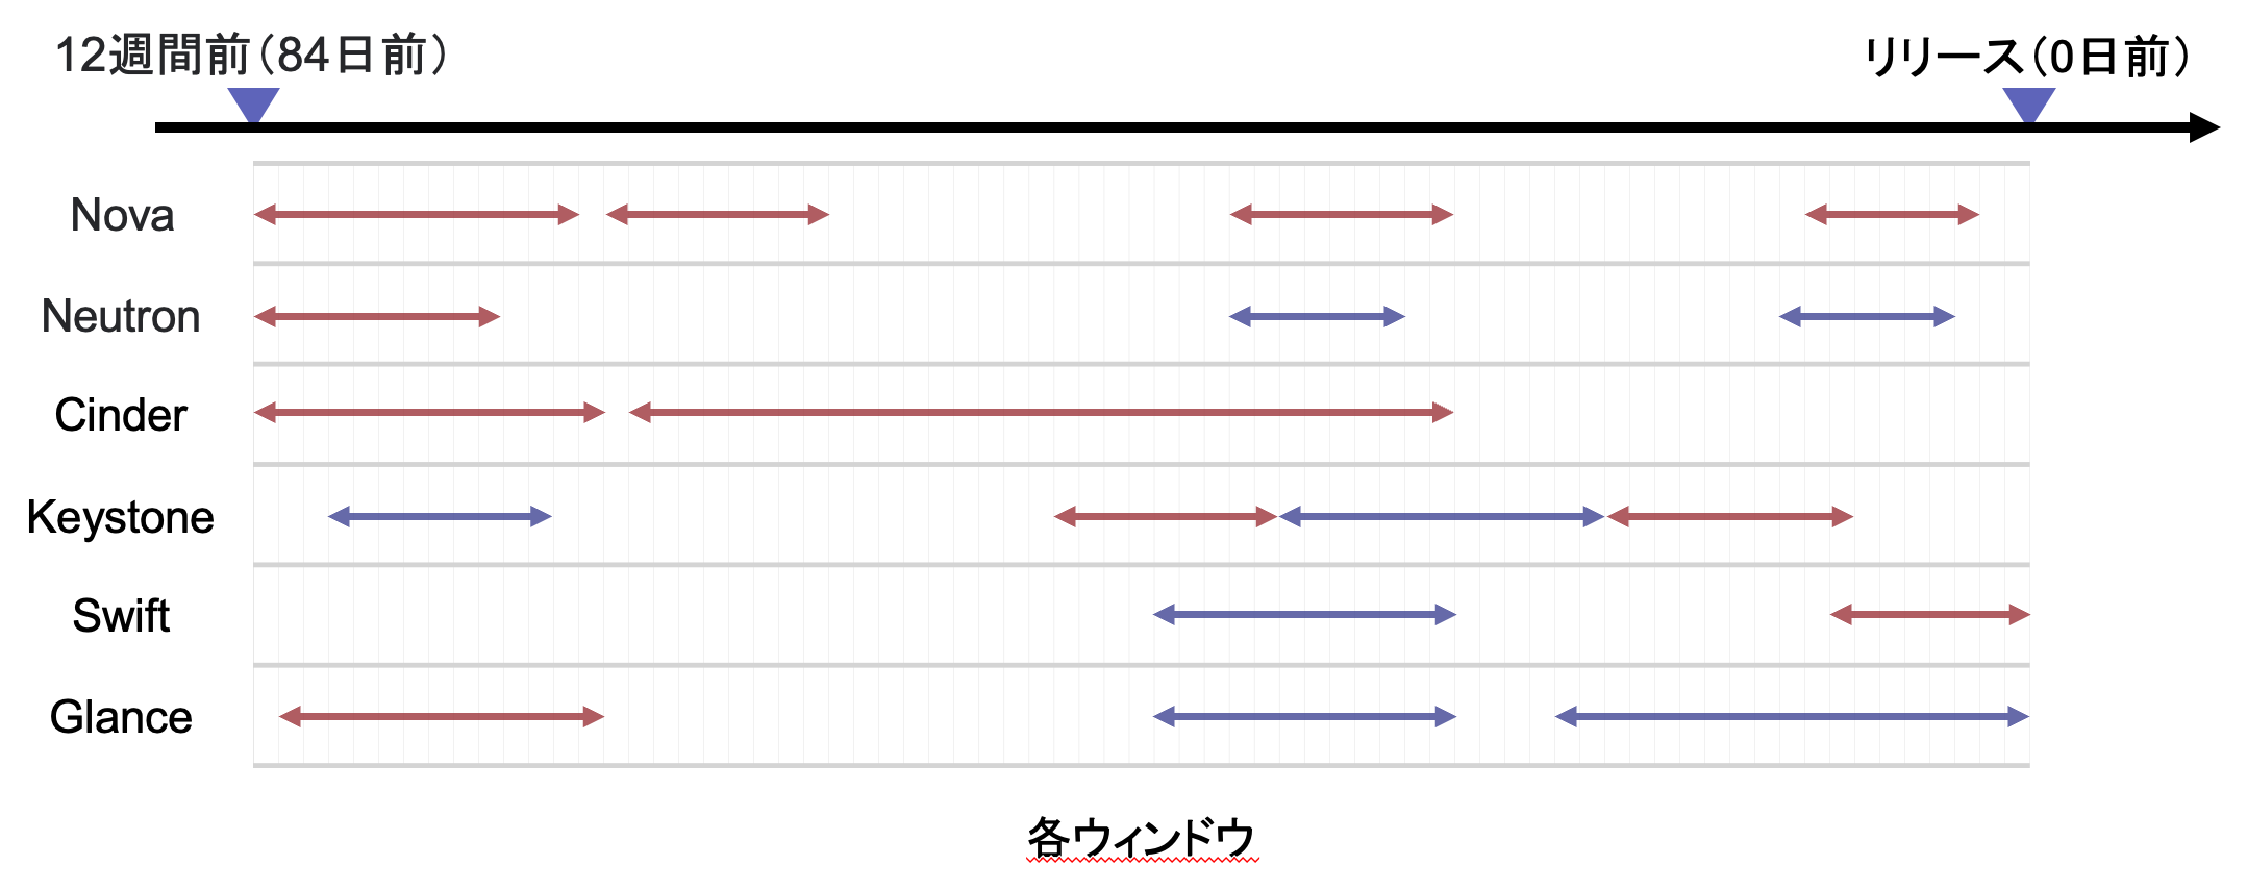
\includegraphics[width=1.0\textwidth]{Uenaka_fig/RQ1_result/review_f1_window.pdf}
    \caption{検証予測モデルの予測結果:7つ以上の連続したウィンドウにおいて提案モデルのF値がベースラインモデルのF値と比べて向上した(赤)または低下した(青)期間}
    \label{fig:review_f1_window}
\end{center}
\end{figure}
%-----------------------

\subsubsection{知見2:検証が開始されるチケットの予測において,開発状況を学習することで,Nova,Cinderプロジェクトではリリース期間内の広範囲,Neutron,Glanceプロジェクトでは前期,Swiftプロジェクトでは後期において提案モデルのF値が向上し,Keystoneプロジェクトでは中期および後期は提案モデルのF値が向上または低下する}
本知見では,リリース期間を前期(リリースが遠い時)・中期(リリース中頃)・後期(リリースが近い時)の3つに分割し,開発状況の学習有無による検証予測モデルの予測性能が異なるかを明らかにする.図\ref{fig:review_f1_window}から,前期は4プロジェクト (Nova, Neutron, Cinder, Glance) ,中期は3プロジェクト (Nova, Cinder, Keystone) ,後期は3プロジェクト (Nova, Keystone, Swift) において,提案モデルのF値がベースラインモデルのF値と比べて向上するという結果が得られた.また,前期は1プロジェクト (Keystone) ,中期は4プロジェクト (Neutron, Keystone, Swift, Glance) ,後期は2プロジェクト (Neutron, Glance) において,提案モデルのF値がベースラインモデルのF値と比べて低下するという結果が得られた.以下に共通の傾向を持つプロジェクトの結果をまとめる.

\textbf{ (Nova, Cinder) }リリース期間内の広範囲で提案モデルのF値が向上したため,これらのプロジェクトではリリース期間内の広範囲において,検証者が検証を開始するチケットが開発状況によって変化していることが示唆される.

\textbf{ (Neutron, Glance) }前期は提案モデルのF値が向上した一方,中期および後期は提案モデルのF値が低下した.よって,これらのプロジェクトでは前期において,検証者が検証を開始するチケットが開発状況によって変化していることが示唆される.

\textbf{ (Swift) }後期は提案モデルのF値が向上した一方,中期は提案モデルのF値が低下した.よって,Swiftプロジェクトでは後期において,検証者が検証を開始するチケットが開発状況によって変化していることが示唆される.

\textbf{ (Keystone) }中期および後期は提案モデルのF値が向上または低下した.よって,Keystoneプロジェクトでは中期および後期の一部の期間において,検証者が検証を開始するチケットが開発状況によって変化していることが示唆される.

また,適合率および再現率に着目することで,提案モデルでF値が向上した理由を考察する.図\ref{fig:review_p}および図\ref{fig:review_r}から,4プロジェクト (Nova, Cinder, Keystone, Glance) においては,F値が向上した期間の一部分において適合率も向上したという結果が得られた.また,3プロジェクト (Nova, Cinder, Glance) においては,F値が向上した期間の一部分において再現率も向上したという結果が得られた.以下に共通の傾向を持つプロジェクトの結果をまとめる.

\textbf{ (Nova, Cinder, Glance) }適合率と再現率の双方が向上したため,開発状況の変化によって検証者が検証を開始するようになるチケットと検証を開始しないようになるチケットが存在し,提案モデルは開発状況を学習することでそれらのチケットを正しく判別したため,F値が向上したと考えられる.

\textbf{ (Keystone) }適合率が向上したため,開発状況の変化によって検証者が検証を開始しないようになるチケットが存在し,提案モデルは開発状況を学習することでそれらのチケットを正しく判別したため,F値が向上したと考えられる.

%図\ref{fig:review_nova_neutron}の結果から,Novaプロジェクトでは,ウィンドウ1〜13,15〜23,40〜48,63〜69において提案モデルのF値が0.01〜0.08高くなり,Neutronプロジェクトでは,ウィンドウ1〜10において提案モデルのF値が0.01〜0.06高くなった.図\ref{fig:review_cinder_keystone}の結果から,Cinderプロジェクトでは,ウィンドウ1〜14,16〜48において提案モデルのF値が0.01〜0.06高くなり,Keystoneプロジェクトでは,ウィンドウ33〜41,55〜64において提案モデルのF値が0.01〜0.11高くなった.図\ref{fig:review_swift_glance}の結果から,Swiftプロジェクトでは,ウィンドウ64〜71において提案モデルのF値が0.04〜0.16高くなり,Glanceプロジェクトでは,ウィンドウ2〜14において提案モデルのF値が0.01〜0.06高くなった.これらの結果から,リリースが遠い時はNova,Neutron,Cinder,Glanceプロジェクト,リリース中頃はNova,Cinder,Keystoneプロジェクト,リリースが近い時はNova,Keystone,SwiftプロジェクトのF値が向上したため,各プロジェクトはそれぞれのリリースまでの期間において,開発状況によって検証判断が変化することが示唆される.


%-----------------------
\begin{figure}[H]
\begin{minipage}{\textwidth}
\vspace{0.08\textheight}
\begin{center}
    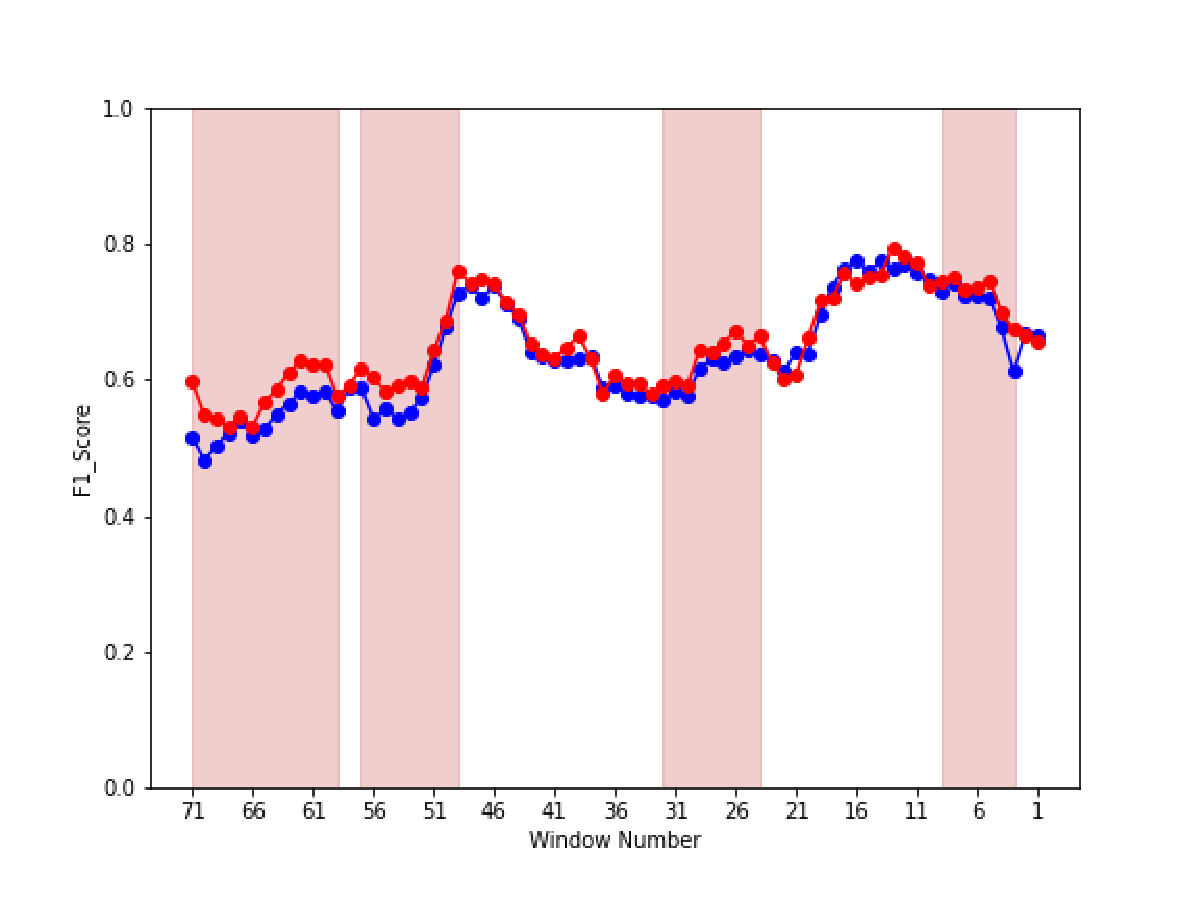
\includegraphics[width=0.495\textwidth]{Uenaka_fig/RQ1_result/Nova_review_F1.pdf}
    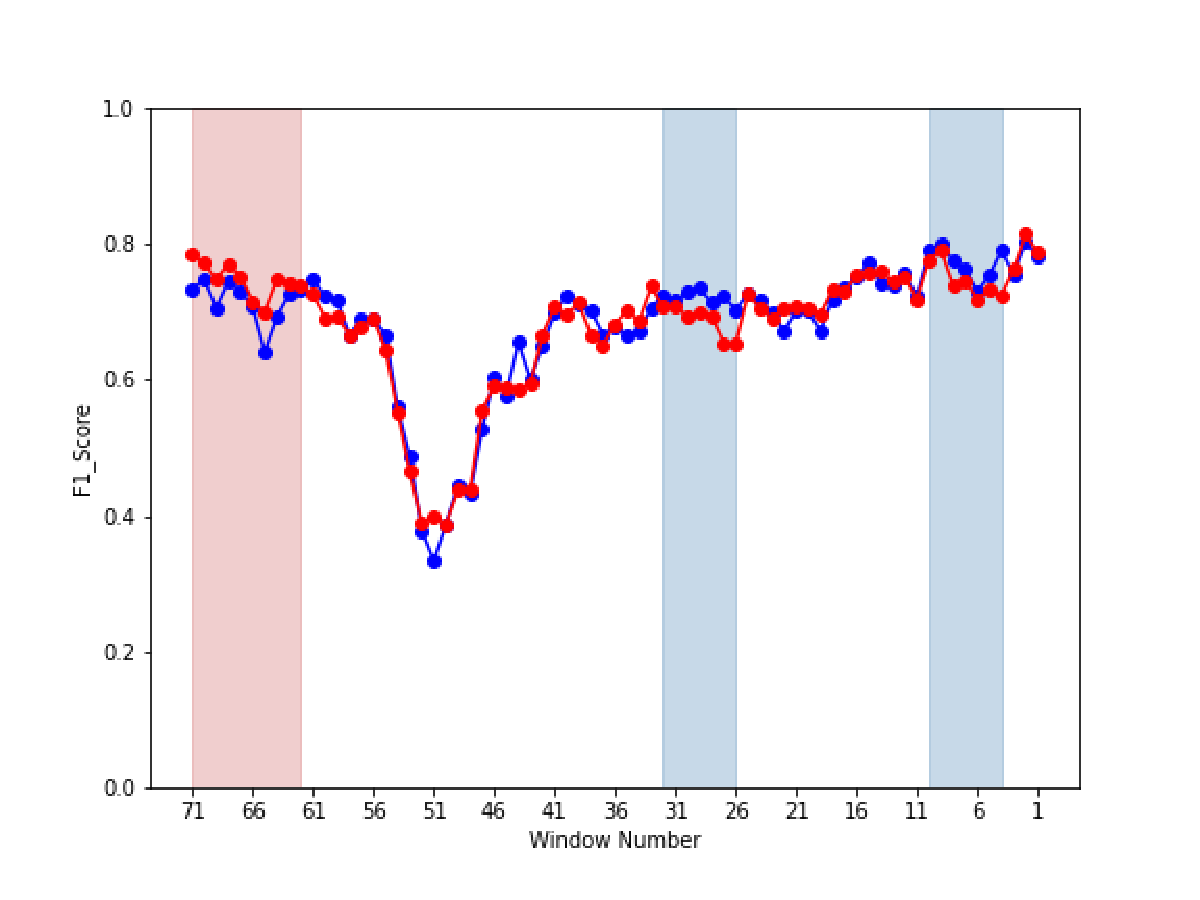
\includegraphics[width=0.495\textwidth]{Uenaka_fig/RQ1_result/Neutron_review_F1.pdf}
    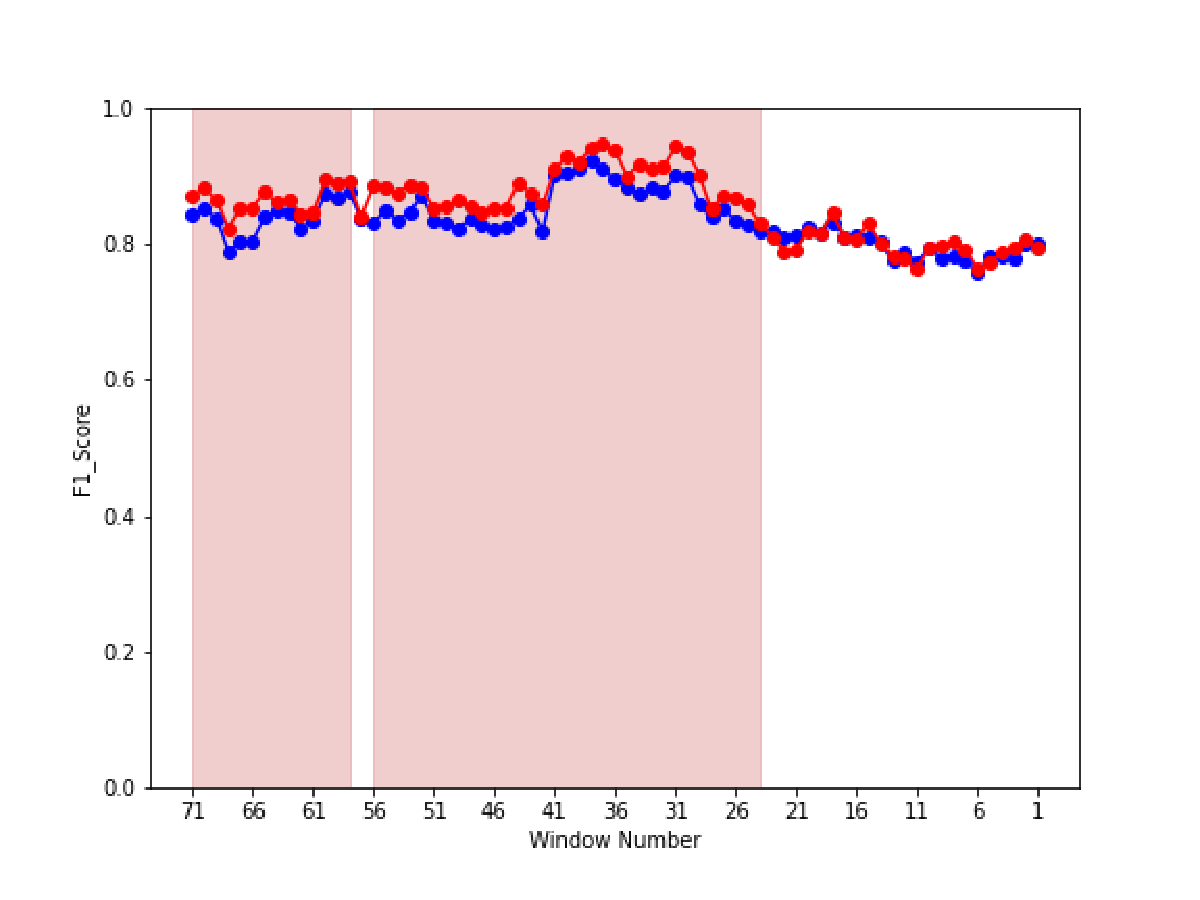
\includegraphics[width=0.495\textwidth]{Uenaka_fig/RQ1_result/Cinder_review_F1.pdf}
    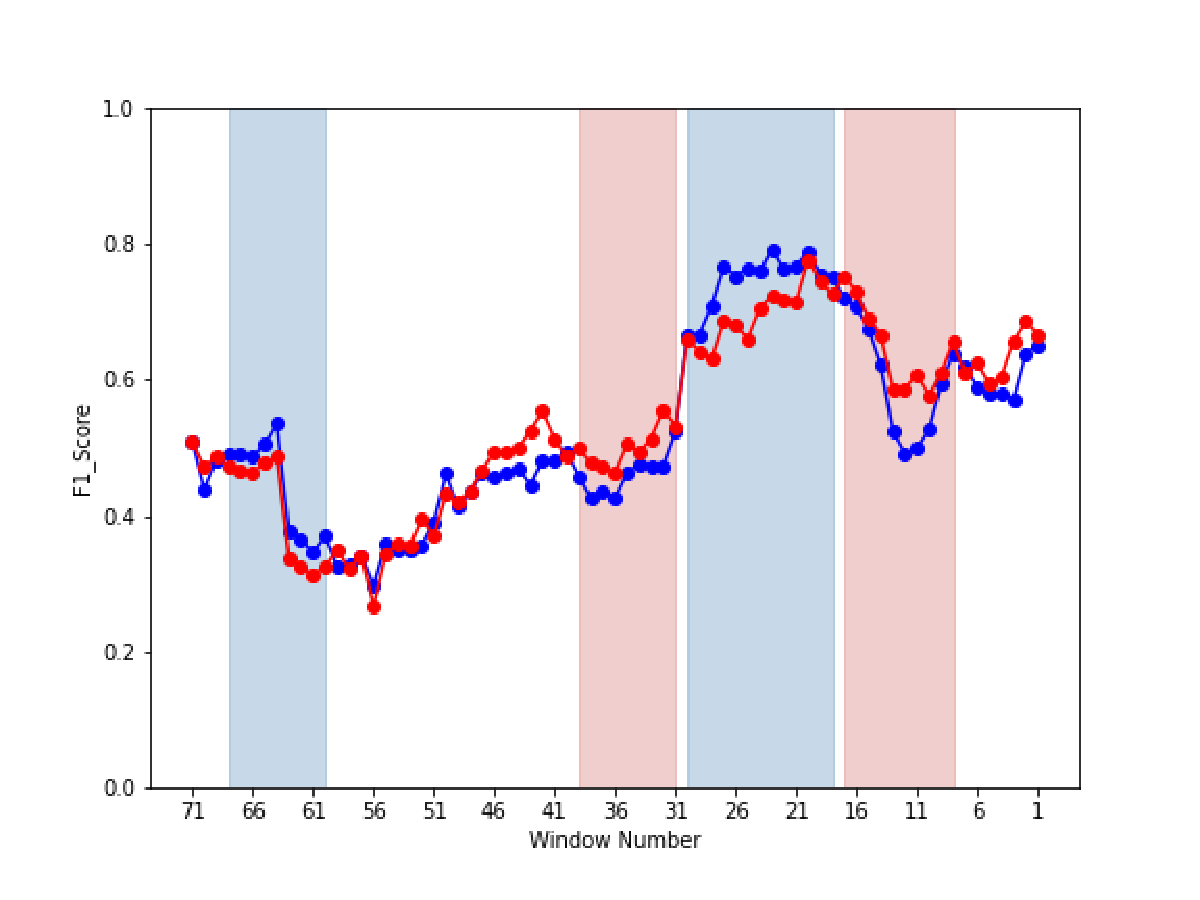
\includegraphics[width=0.495\textwidth]{Uenaka_fig/RQ1_result/Keystone_review_F1.pdf}
    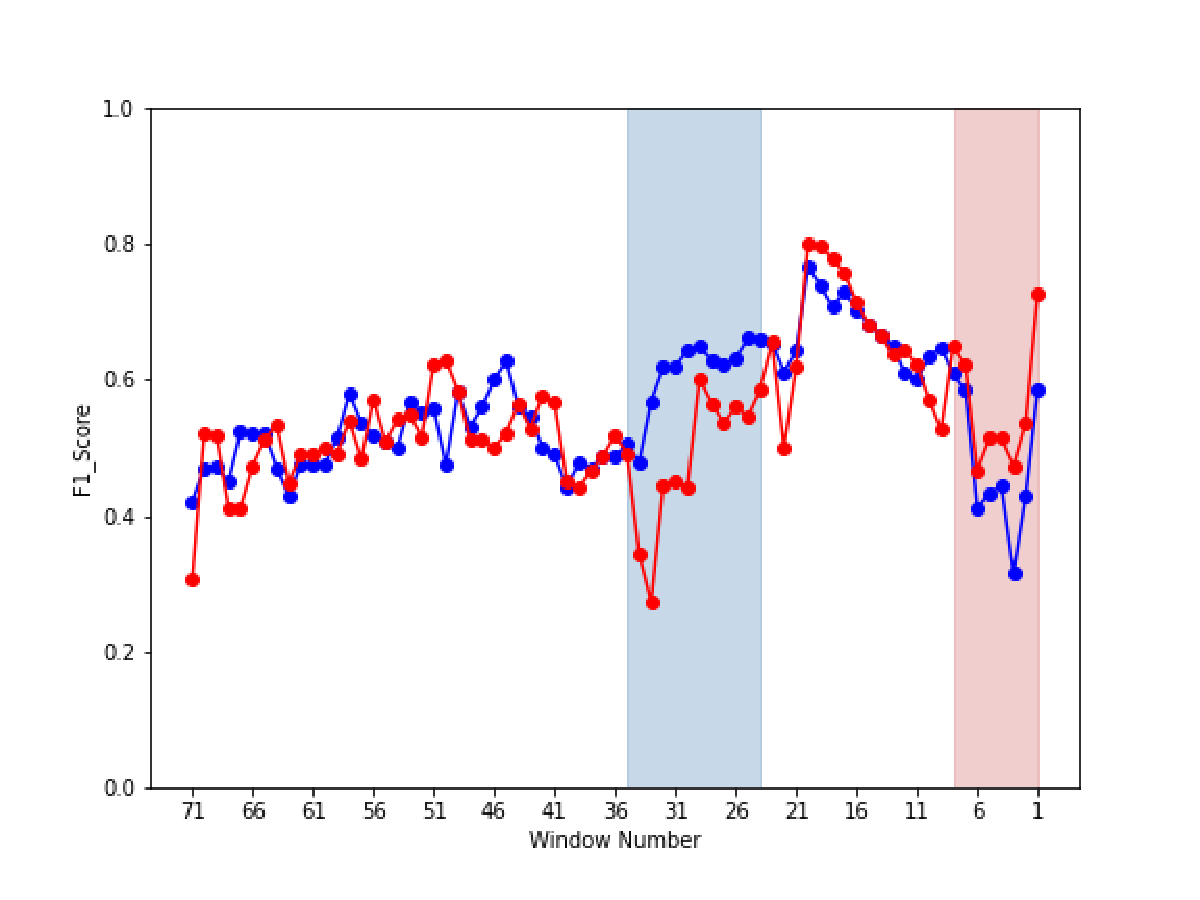
\includegraphics[width=0.495\textwidth]{Uenaka_fig/RQ1_result/Swift_review_F1.pdf}
    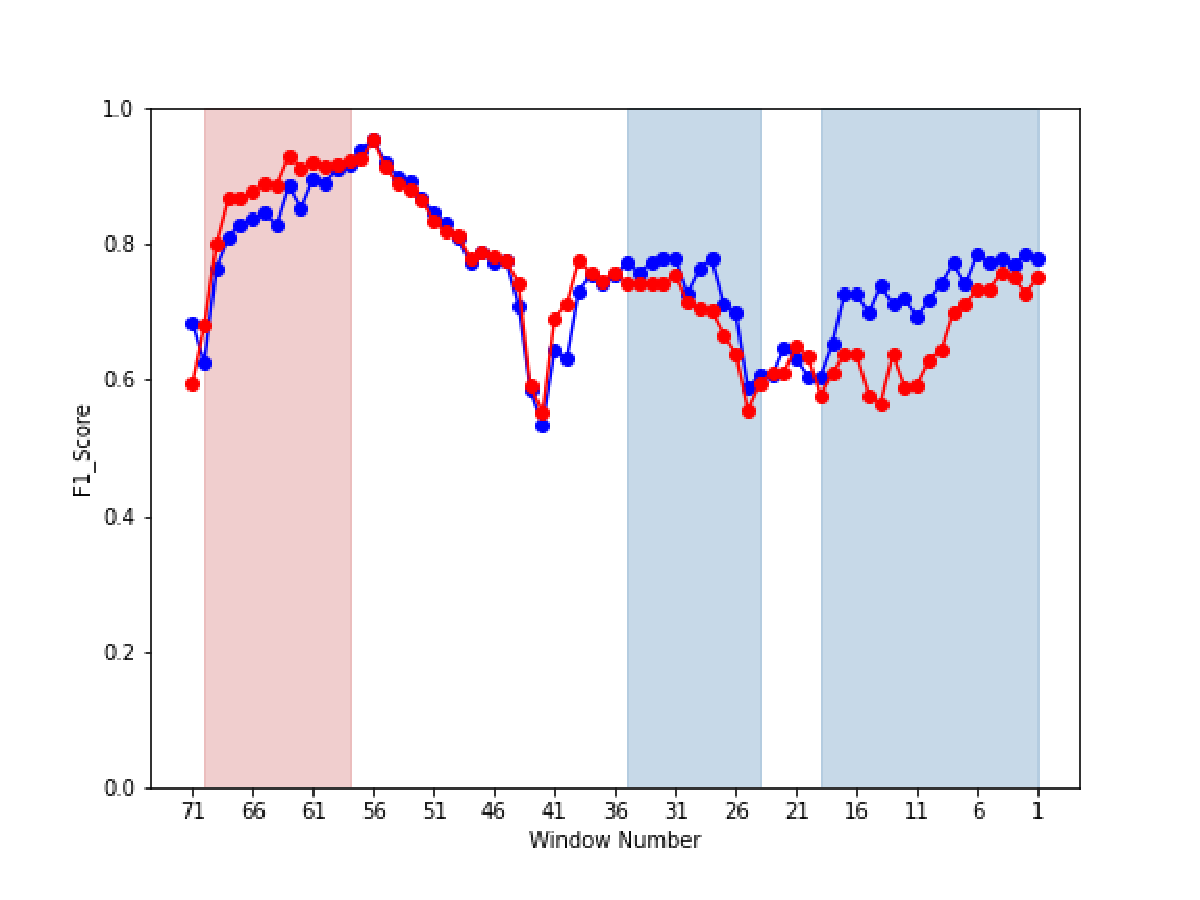
\includegraphics[width=0.495\textwidth]{Uenaka_fig/RQ1_result/Glance_review_F1.pdf}
    \caption{検証予測モデルのF値(上段左:Nova,上段右:Neutron,中段左:Cinder,\\ 中段右:Keystone,下段左:Swift,下段右:Glance)(赤:提案モデル,青:ベースラインモデル)}
    \label{fig:review_f}
\end{center}
\vspace{0.08\textheight}
\end{minipage}
\end{figure}
%-----------------------

%-----------------------
\begin{figure}[H]
\begin{minipage}{\textwidth}
\vspace{0.08\textheight}
\begin{center}
    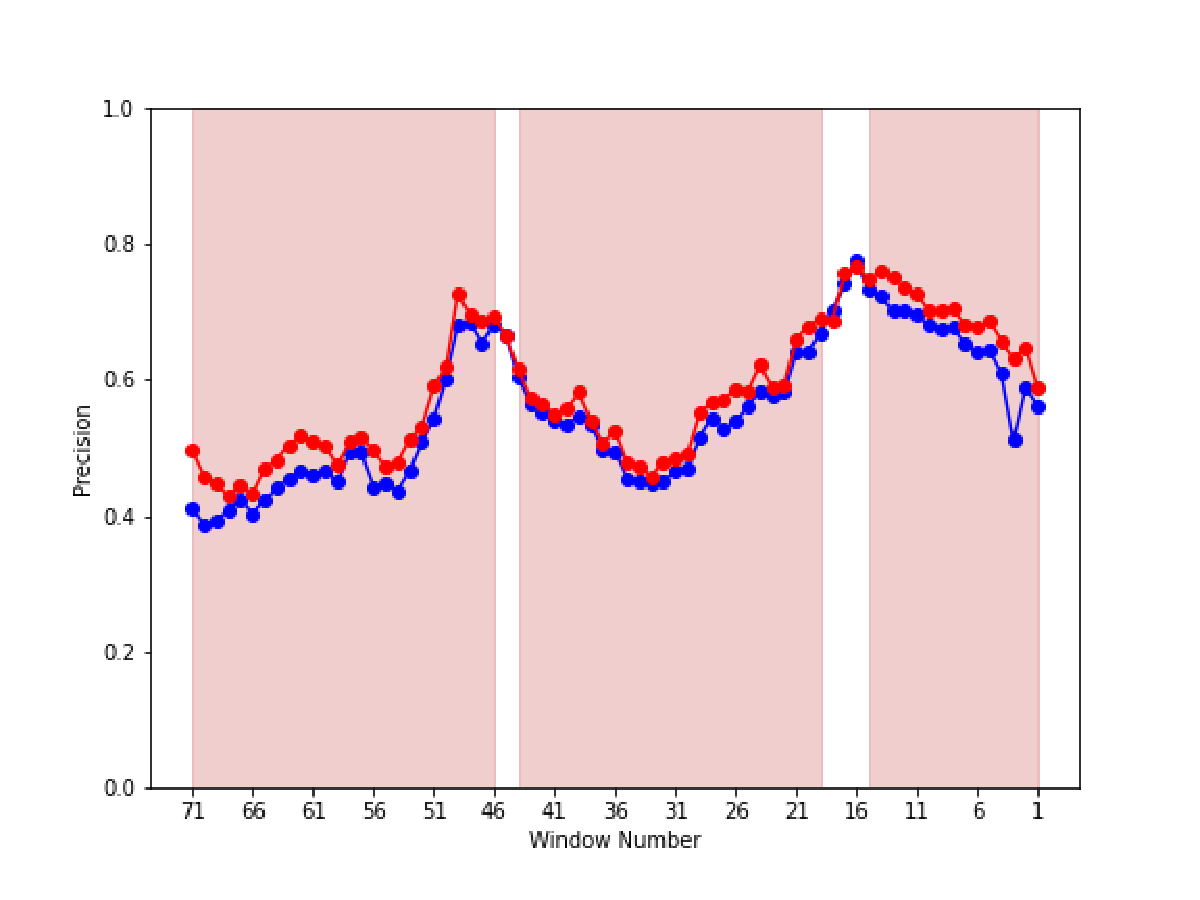
\includegraphics[width=0.495\textwidth]{Uenaka_fig/RQ1_result/Nova_review_Precision.pdf}
    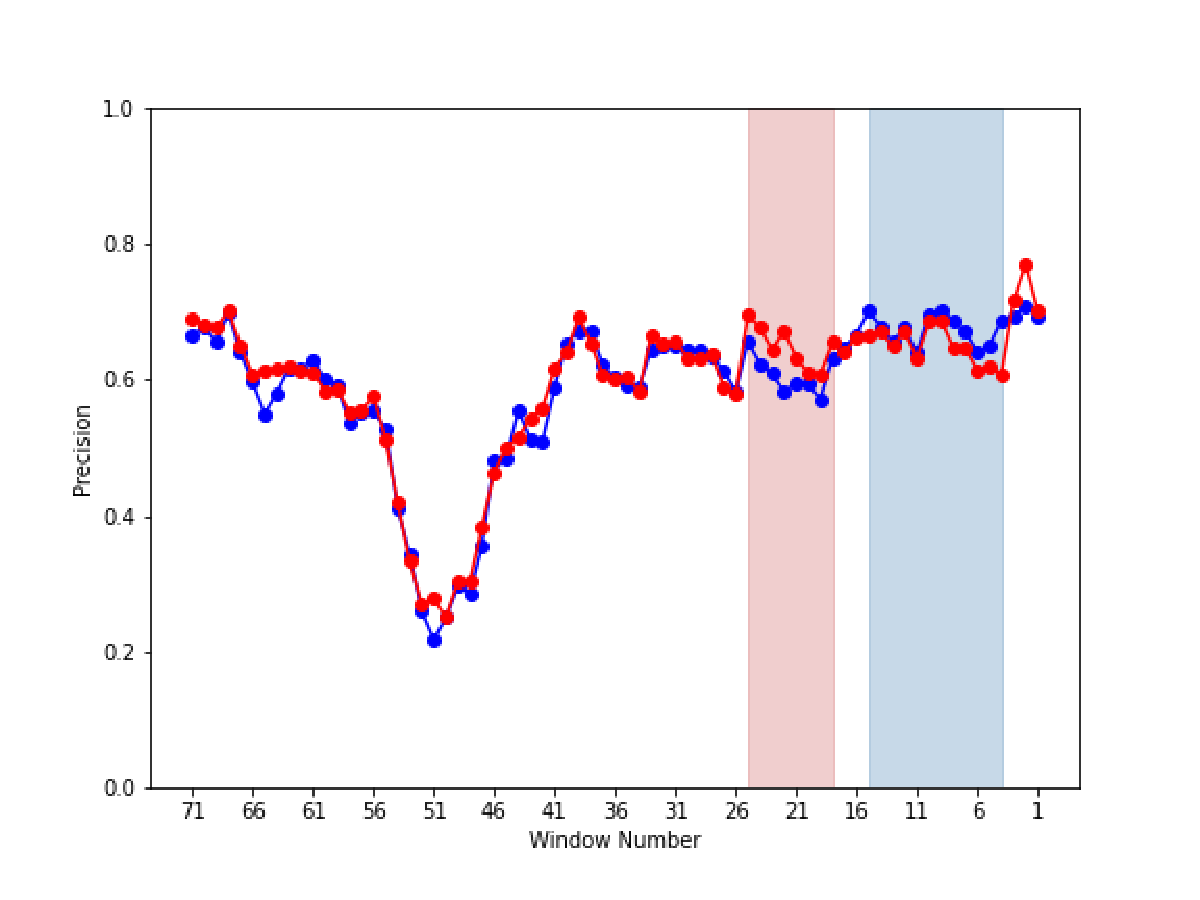
\includegraphics[width=0.495\textwidth]{Uenaka_fig/RQ1_result/Neutron_review_Precision.pdf}
    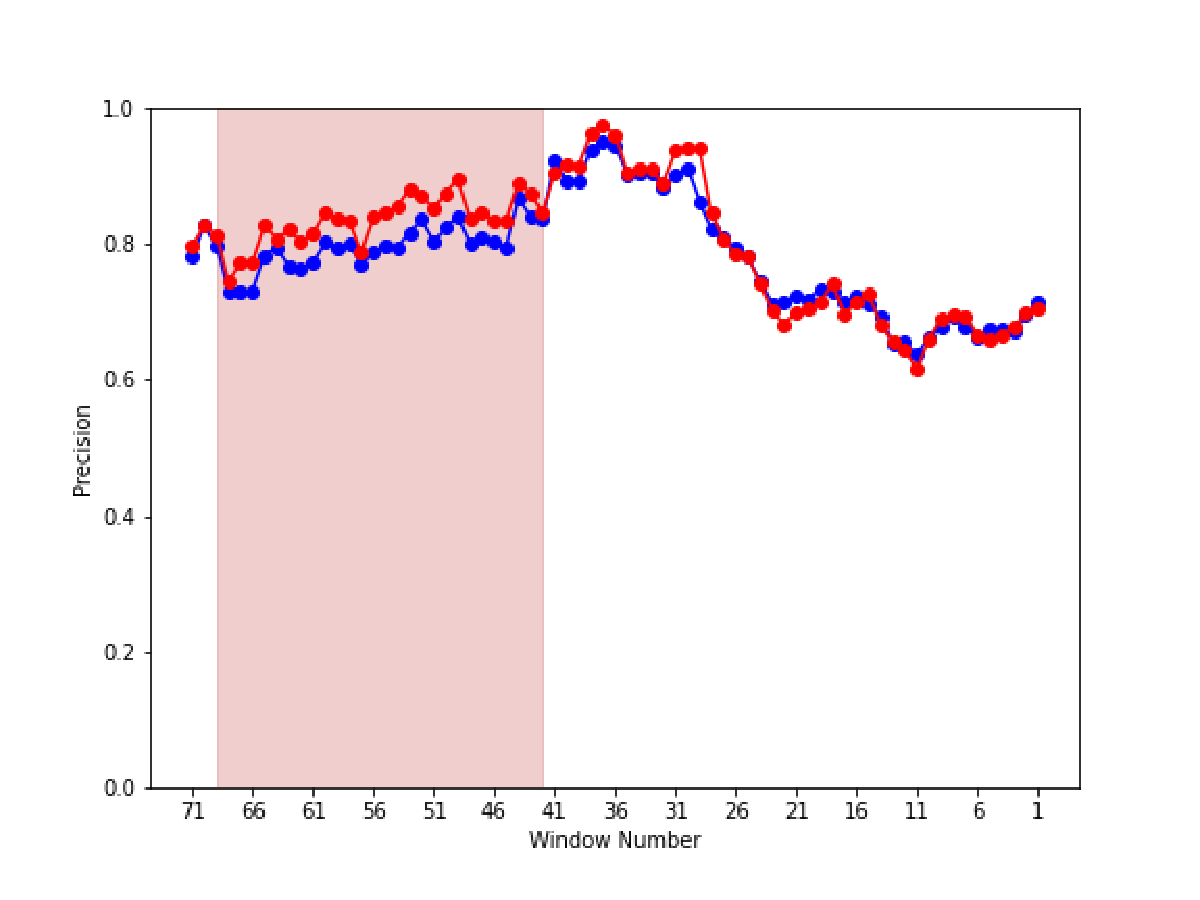
\includegraphics[width=0.495\textwidth]{Uenaka_fig/RQ1_result/Cinder_review_Precision.pdf}
    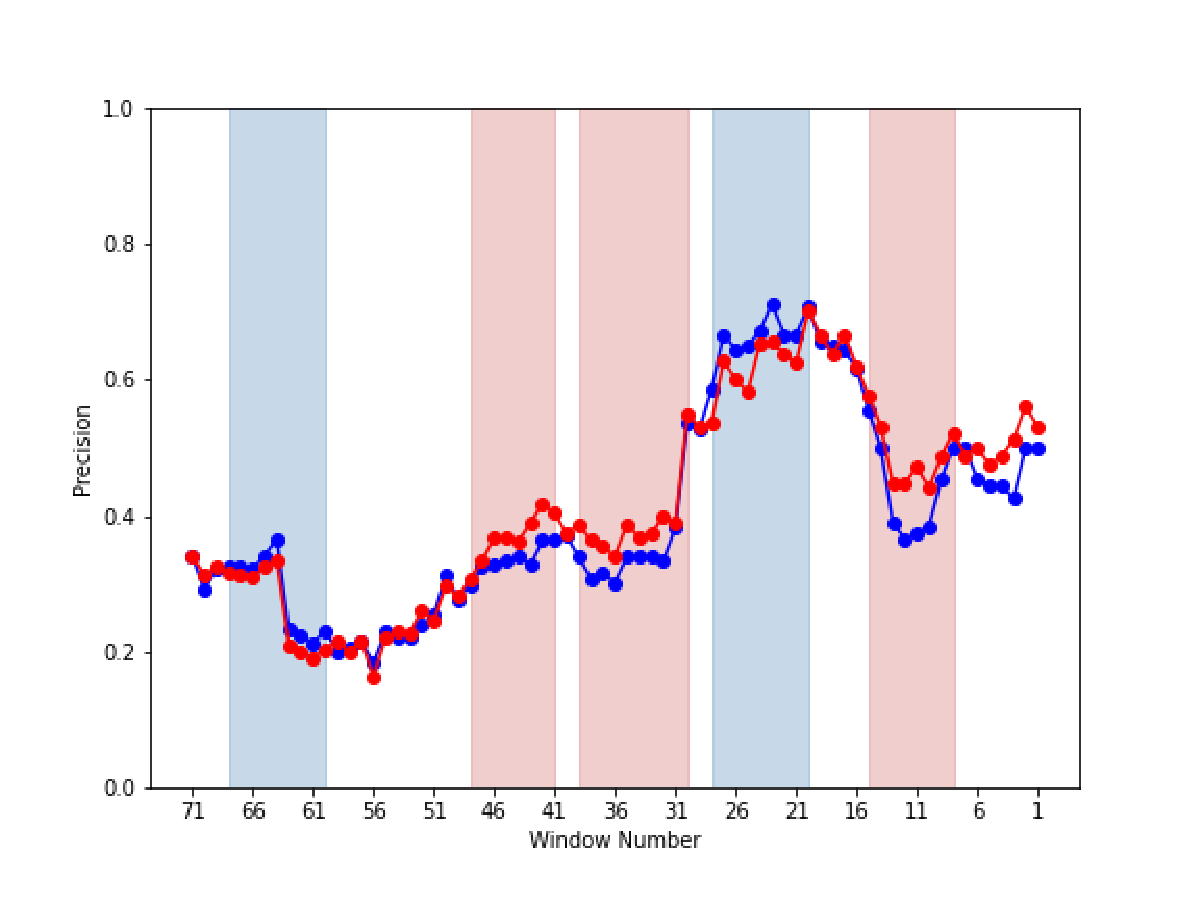
\includegraphics[width=0.495\textwidth]{Uenaka_fig/RQ1_result/Keystone_review_Precision.pdf}
    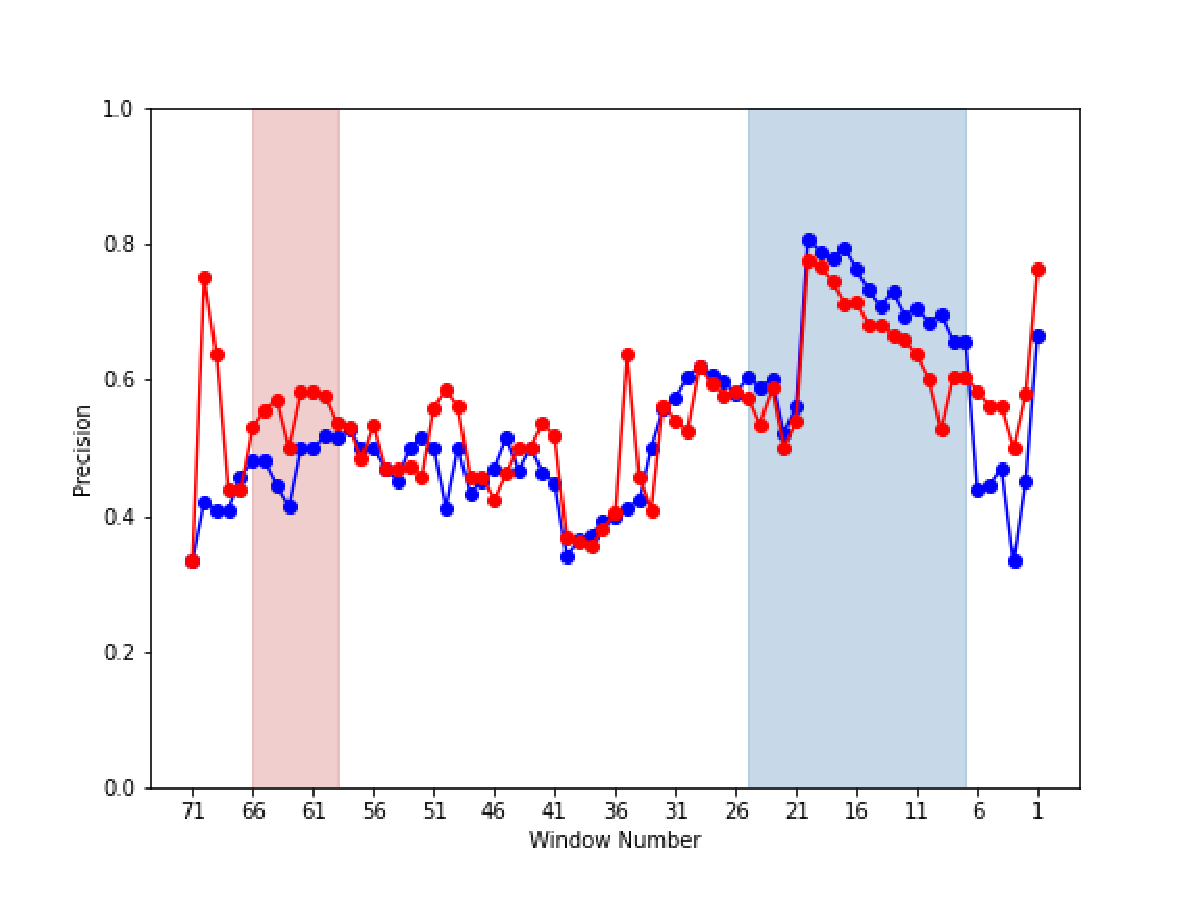
\includegraphics[width=0.495\textwidth]{Uenaka_fig/RQ1_result/Swift_review_Precision.pdf}
    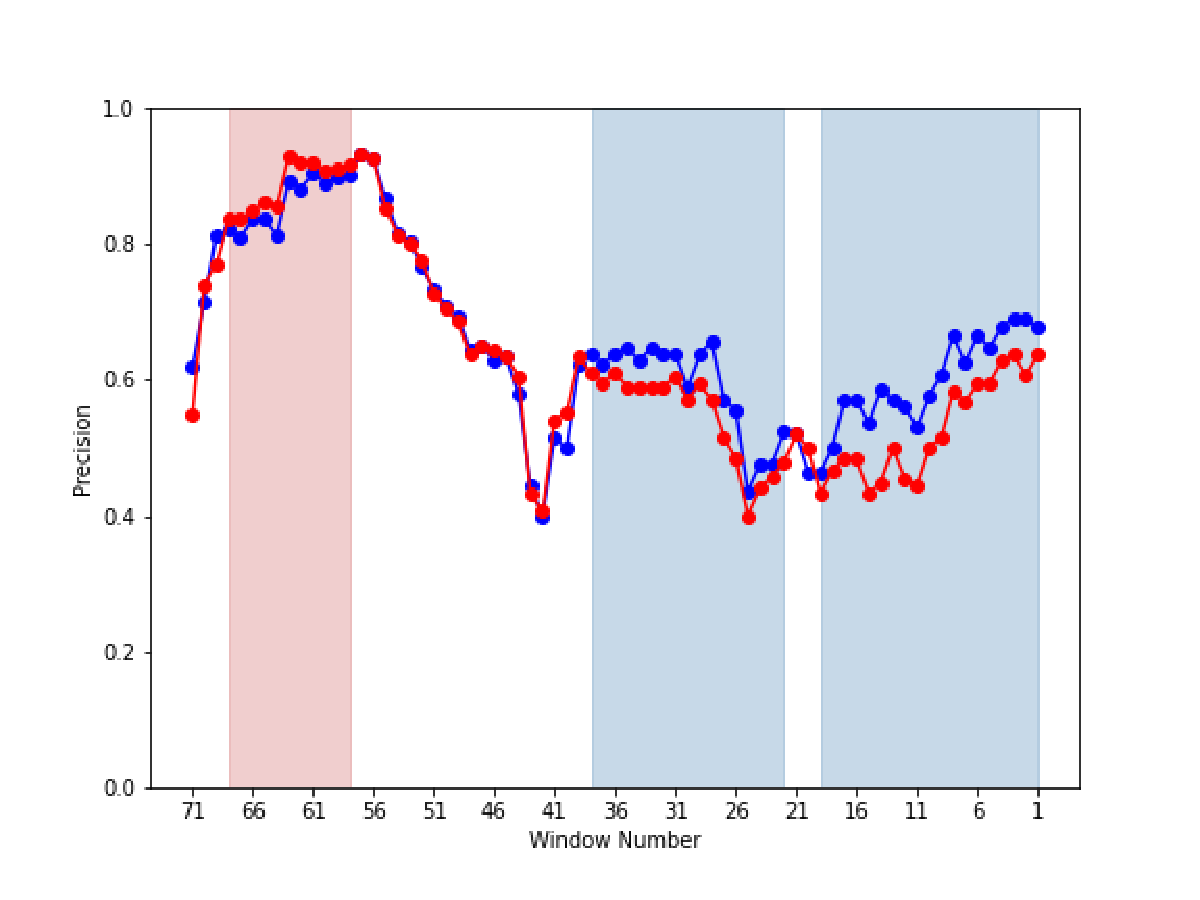
\includegraphics[width=0.495\textwidth]{Uenaka_fig/RQ1_result/Glance_review_Precision.pdf}
    \caption{検証予測モデルの適合率(上段左:Nova,上段右:Neutron,中段左:Cinder,\\ 中段右:Keystone,下段左:Swift,下段右:Glance)(赤:提案モデル,青:ベースラインモデル)}
    \label{fig:review_p}
\end{center}
\vspace{0.08\textheight}
\end{minipage}
\end{figure}
%-----------------------

%-----------------------
\begin{figure}[H]
\begin{center}
    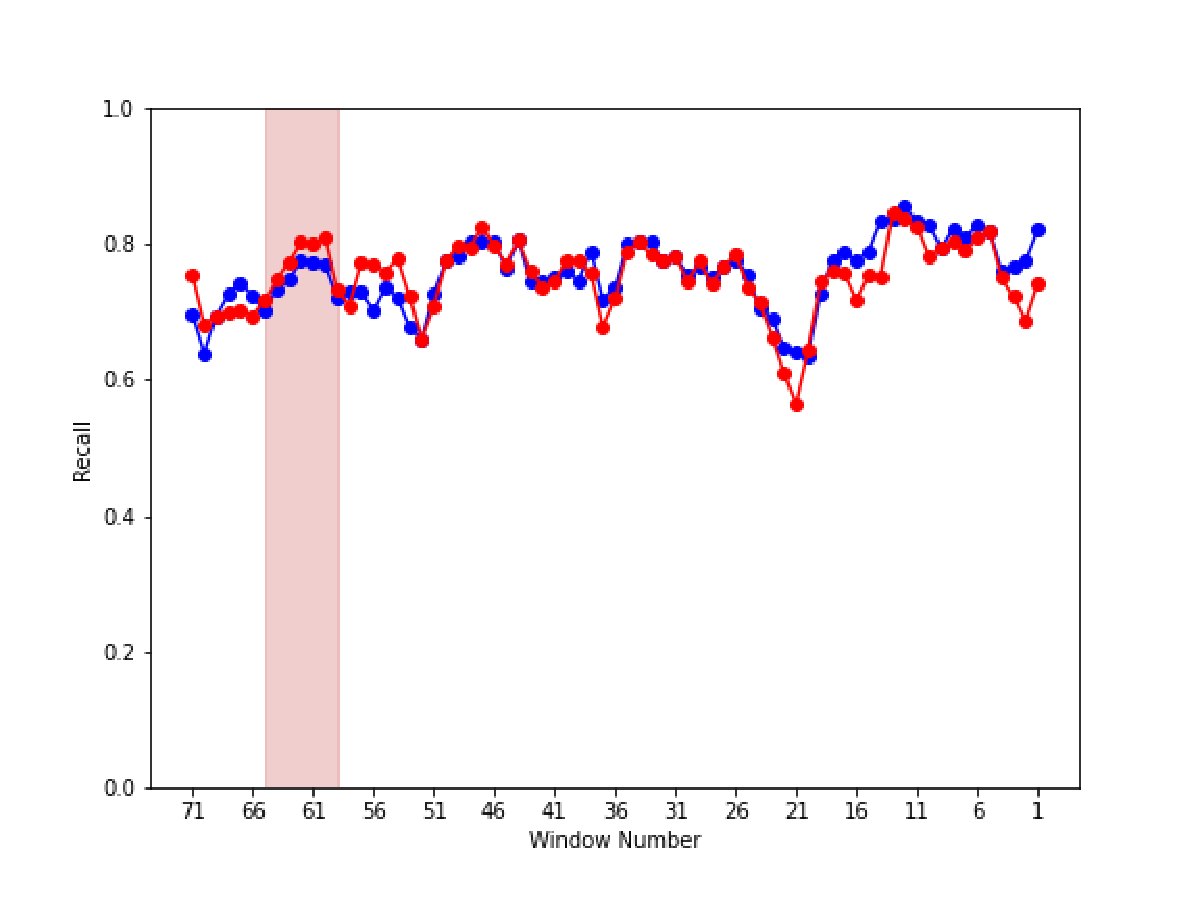
\includegraphics[width=0.495\textwidth]{Uenaka_fig/RQ1_result/Nova_review_Recall.pdf}
    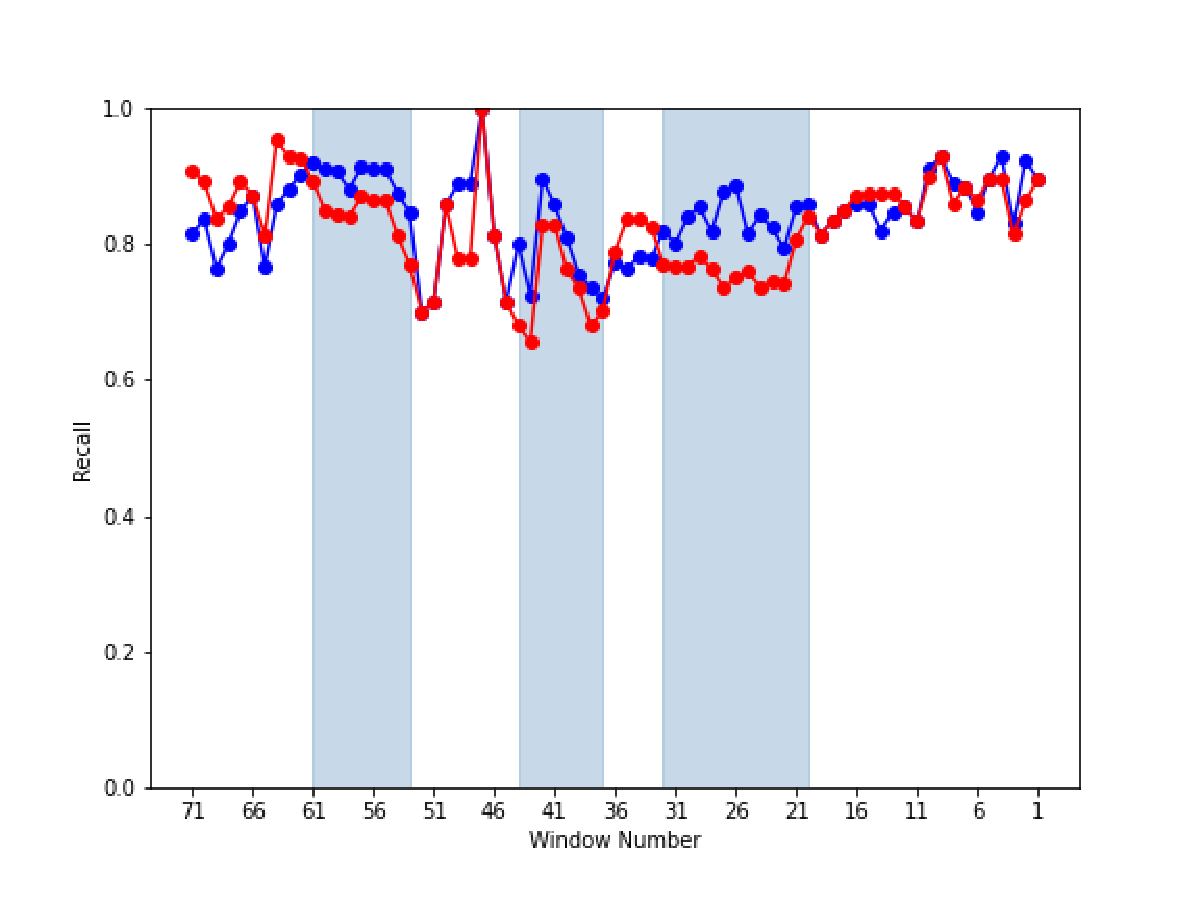
\includegraphics[width=0.495\textwidth]{Uenaka_fig/RQ1_result/Neutron_review_Recall.pdf}
    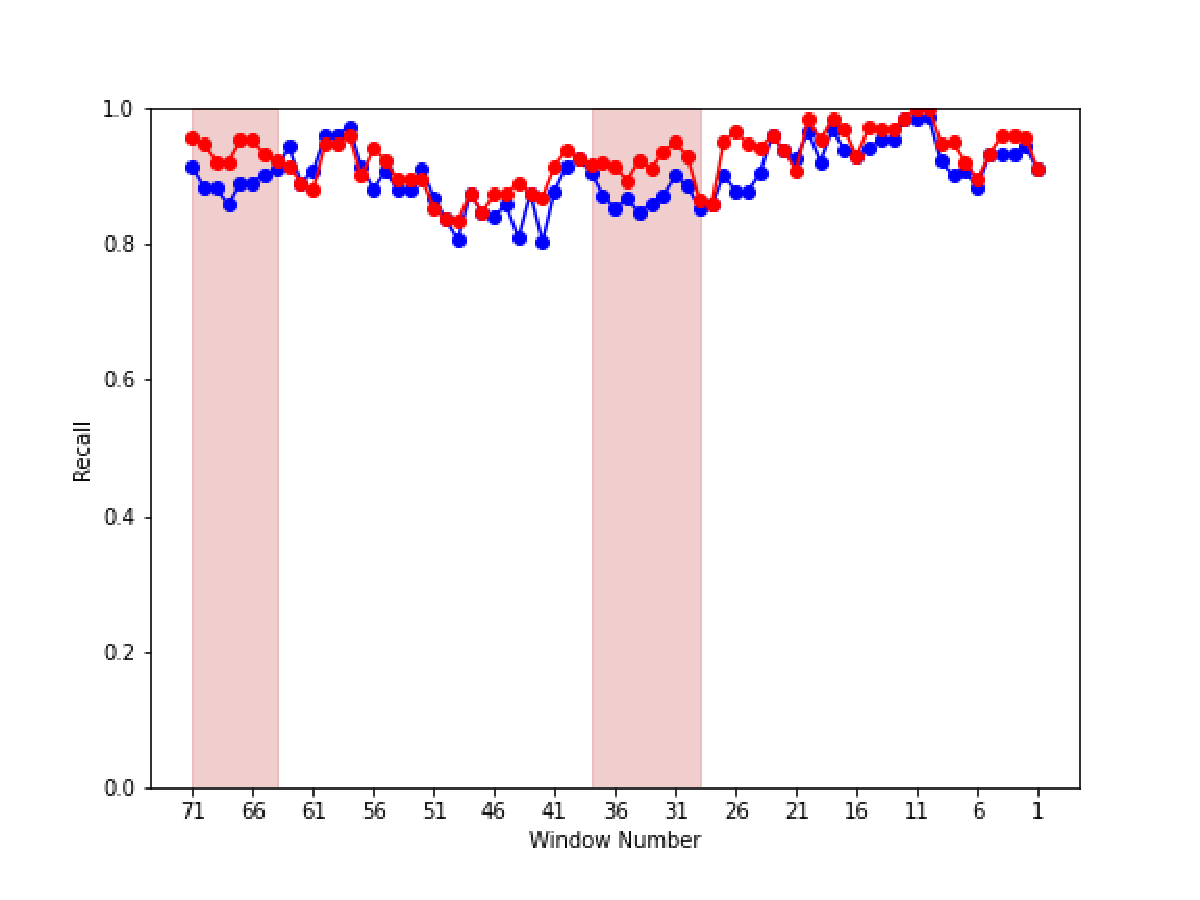
\includegraphics[width=0.495\textwidth]{Uenaka_fig/RQ1_result/Cinder_review_Recall.pdf}
    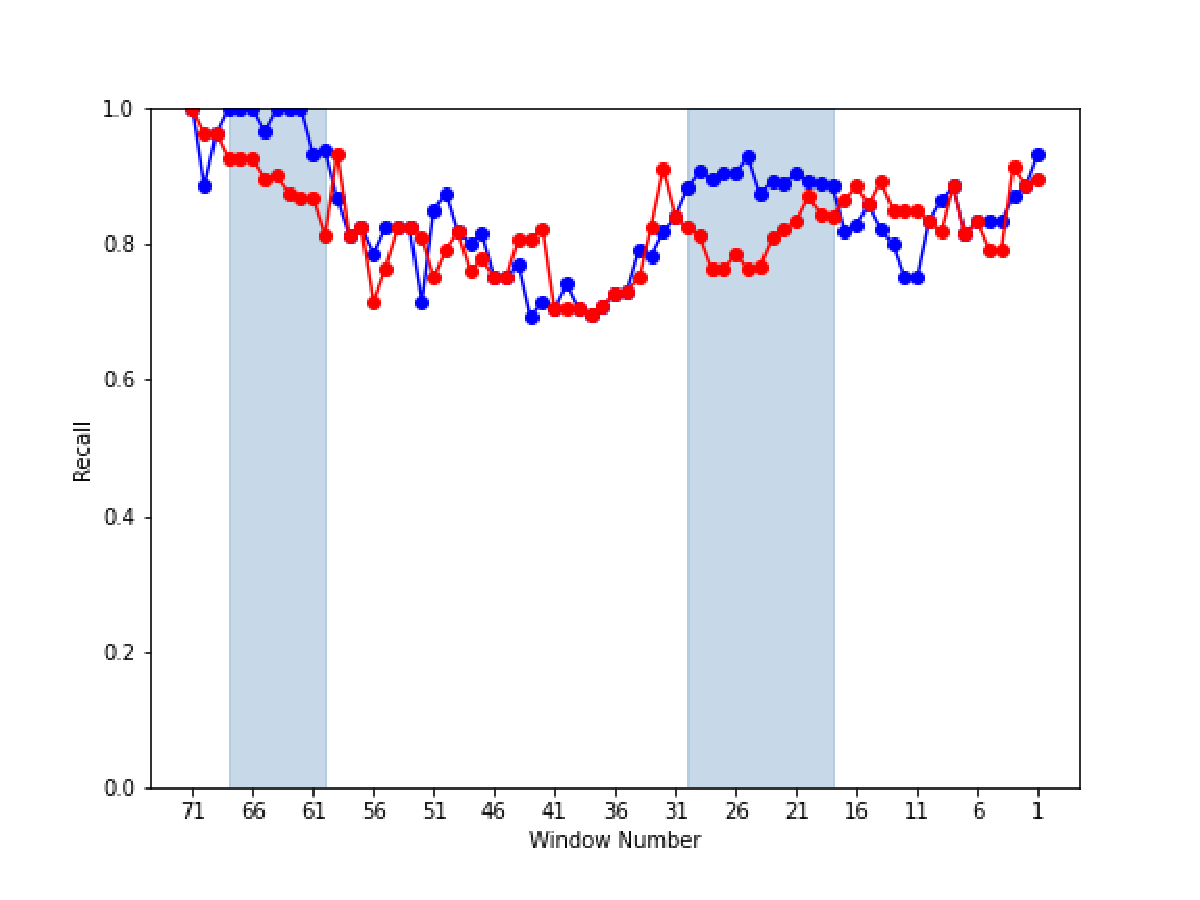
\includegraphics[width=0.495\textwidth]{Uenaka_fig/RQ1_result/Keystone_review_Recall.pdf}
    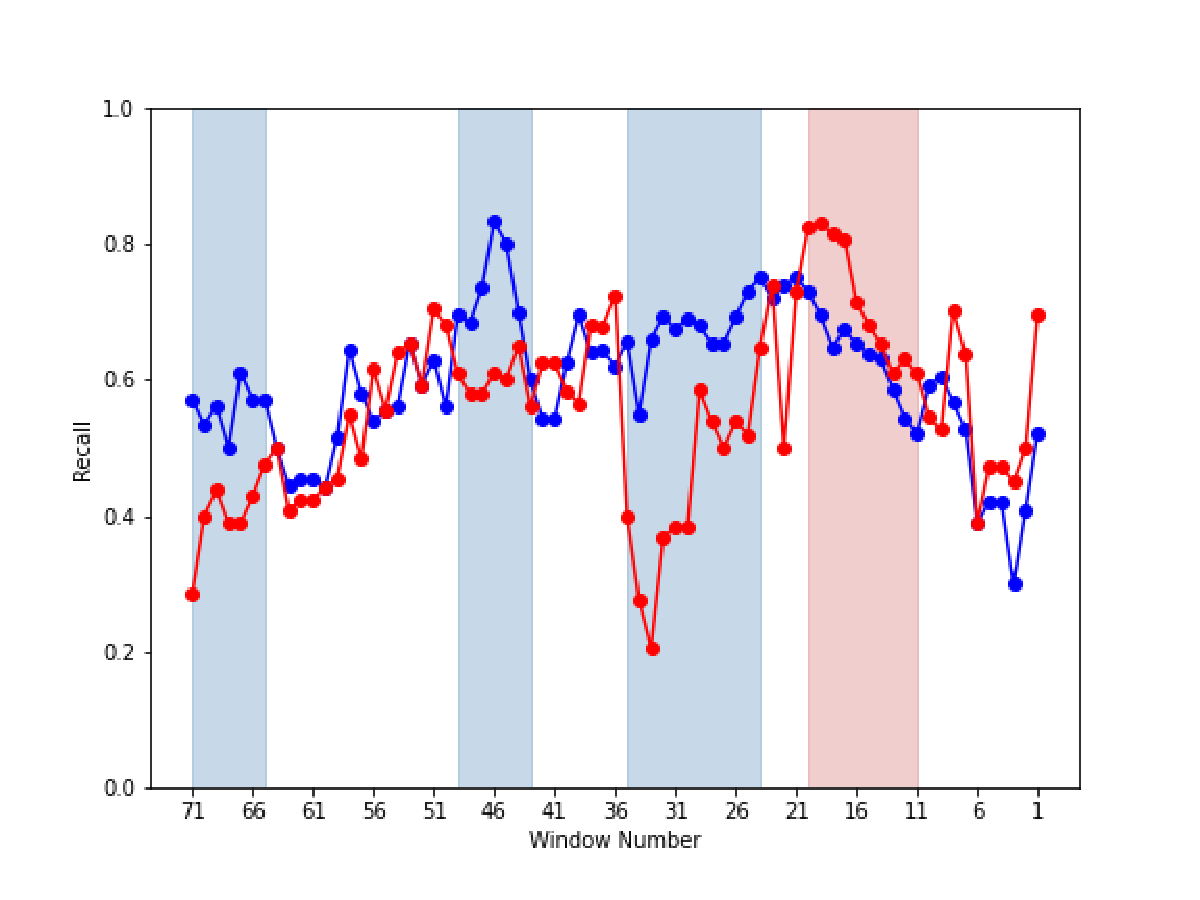
\includegraphics[width=0.495\textwidth]{Uenaka_fig/RQ1_result/Swift_review_Recall.pdf}
    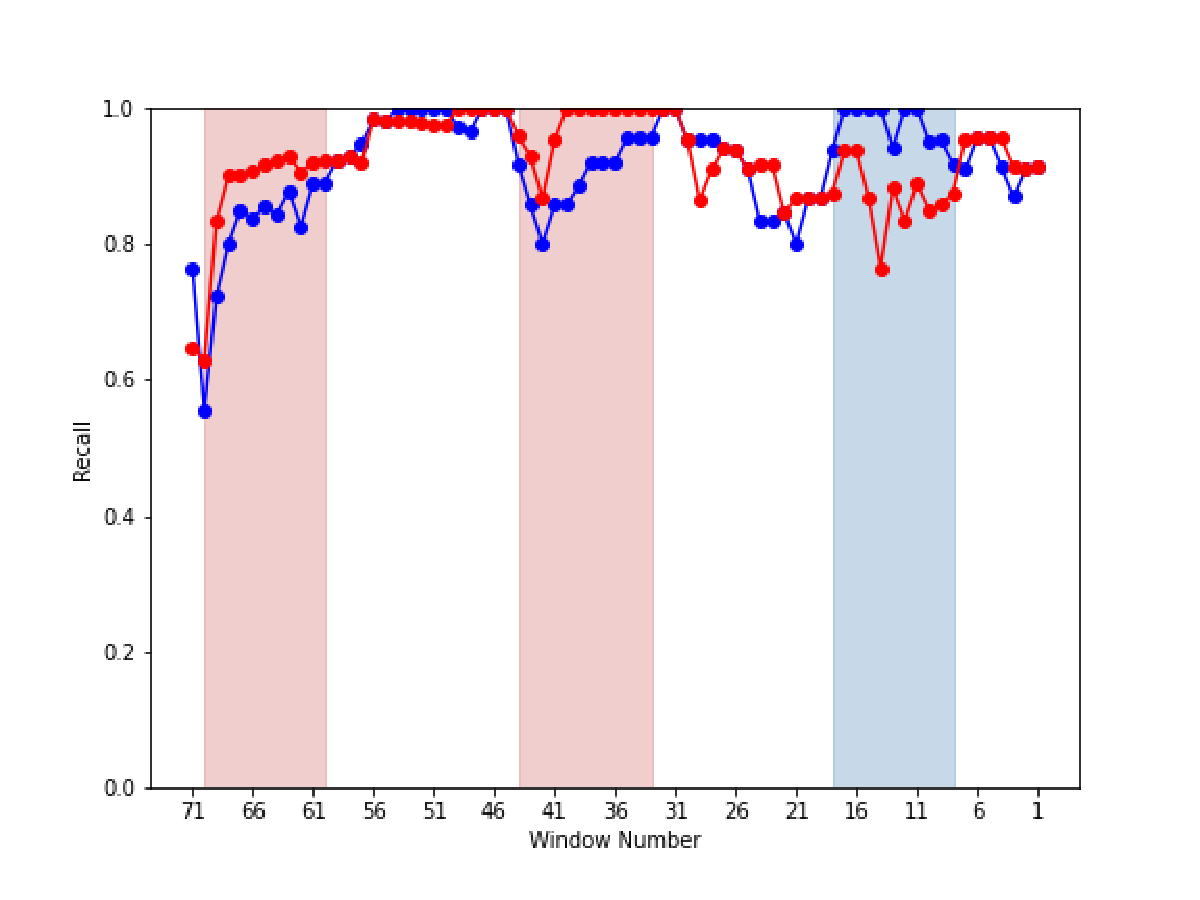
\includegraphics[width=0.495\textwidth]{Uenaka_fig/RQ1_result/Glance_review_Recall.pdf}
    \caption{検証予測モデルの再現率(上段左:Nova,上段右:Neutron,中段左:Cinder,\\ 中段右:Keystone,下段左:Swift,下段右:Glance)(赤:提案モデル,青:ベースラインモデル)}
    \label{fig:review_r}
\end{center}
\end{figure}
%-----------------------


\subsection{導入予測モデル}\label{sec:rq1_donyu}
各プロジェクトの導入予測モデルの予測結果として,図\ref{fig:merge_f}はF値,図\ref{fig:merge_p}は適合率,図\ref{fig:merge_r}は再現率を示す.図の縦軸および横軸や折れ線,図の配置や色で表されている期間の定義は\ref{sec:rq1_kenshou}項と同様であり,図\ref{fig:merge_f1_window}の定義も\ref{sec:rq1_kenshou}項と同様である.また,表\ref{table:merge_seino_jikeiretsu}はベースラインモデルの予測性能の時系列変化の分析結果として,各プロジェクトの導入予測モデルにおける評価指標の回帰係数の分類を示す.表\ref{table:merge_seino_jikeiretsu}において,回帰係数の分類は表\ref{table:review_seino_jikeiretsu}と同様の矢印で表す.

\subsubsection{知見3:導入されるチケットの予測において,リリースが近づくにつれて,3プロジェクト (Nova, Neutron, Cinder) ではベースラインモデルの予測性能が向上し,2プロジェクト (Keystone, Swift) では低下し,1プロジェクト (Glance) では変化しない}
本知見では,知見1と同様にリリースまでの期間内での導入予測モデルの予測性能の変化を分析した.表\ref{table:merge_seino_jikeiretsu}の回帰係数の分類から,ベースラインモデルの全ての評価指標は2プロジェクト (Neutron, Cinder) において回帰係数が有意に増加し,Swiftプロジェクトにおいて回帰係数が有意に減少し,Glanceプロジェクトにおいて回帰係数が有意に増加および減少しないという結果が得られた.また,NovaプロジェクトではF値および適合率の回帰係数が有意に増加し,再現率の回帰係数が有意に増加および減少しないという結果が得られ,KeystoneプロジェクトではF値および再現率の回帰係数が有意に減少し,適合率の回帰係数が有意に増加するという結果が得られた.以下に共通の傾向を持つプロジェクトの結果をまとめる.

\textbf{ (Nova, Neutron, Cinder) }リリースが近づくにつれてベースラインモデルのF値および適合率が向上し,再現率も向上もしくは変化しなかったため,これらのプロジェクトではリリースが近づくにつれてベースラインモデルの予測性能が向上することを明らかにした.このことから,これらの検証者にとって,従来研究\cite{prioritizer}のようなモデル(ベースラインモデル)はリリースが近づくにつれて有用となることが示唆されたため,これらのプロジェクトの検証者はリリースが近づくにつれて,チケットおよびチケット報告者の特徴から導入するチケットを判断する傾向にあることが示唆される.

\textbf{ (Keystone, Swift) }リリースが近づくにつれてベースラインモデルのF値および再現率が低下したため,これらのプロジェクトではリリースが近づくにつれてベースラインモデルの予測性能が低下することを明らかにした.このことから,これらのプロジェクトの検証者にとって,従来研究\cite{prioritizer}のようなモデル(ベースラインモデル)はリリースから遠いタイミングで有用となることが示唆されたため,これらのプロジェクトの検証者はリリースが近づくにつれて,チケットおよびチケット報告者以外の特徴から導入するチケットを判断する傾向にあることが示唆される.

\textbf{ (Glance) }リリースが近づくにつれてベースラインモデルの全ての評価指標の回帰係数が有意に増加および減少しなかったため,Glanceプロジェクトではリリース時期によってベースラインモデルの予測性能が変化しないことを明らかにした.

% よって,ベースラインモデルの予測性能の時系列変化を分析した結果,全ての評価指標の回帰係数が有意に増加したもしくは有意に増加および減少しなかったプロジェクト (Nova, Neutron, Cinder) ,F値および再現率の回帰係数が有意に減少したプロジェクト (Keystone, Swift) ,全ての評価指標の回帰係数が有意に増加および減少しなかったプロジェクト (Glance) の3種類にプロジェクトが分類できるという結果が得られた.

%--------------------
\begin{table*}[t]
\caption{各プロジェクトの導入予測モデルにおける評価指標の回帰係数の分類}
\label{table:merge_seino_jikeiretsu}
\centering
\vspace{0.5zh}
\scalebox{0.9}{
\begin{tabular}{l|c|c|c|c|c|c}
    \hline \hline
    評価指標 & Nova & Neutron & Cinder & Keystone & Swift & Glance \\ \hline
    F値 & $\nearrow$ & $\nearrow$ & $\nearrow$ & $\searrow$ & $\searrow$ & $\rightarrow$ \\ \hline
    適合率 & $\nearrow$ & $\nearrow$ & $\nearrow$ & $\nearrow$ & $\searrow$ & $\rightarrow$ \\ \hline
    再現率 & $\rightarrow$ & $\nearrow$ & $\nearrow$ & $\searrow$ & $\searrow$ & $\rightarrow$ \\ \hline
\end{tabular}}
\end{table*}
%--------------------

%--------------------
% \begin{table*}[t]
% \caption{各プロジェクトの導入予測モデルにおける評価指標の回帰係数の分類}
% \label{table:merge_seino_jikeiretsu}
% \centering
% \vspace{0.5zh}
% \scalebox{0.74}{
% \begin{tabular}{l|cc|cc|cc|cc|cc|cc}
%     \hline \hline
%     \multirow{2}{*}{評価指標} & \multicolumn{2}{c|}{Nova} & \multicolumn{2}{c|}{Neutron} & \multicolumn{2}{c|}{Cinder} & \multicolumn{2}{c|}{Keystone} & \multicolumn{2}{c|}{Swift} & \multicolumn{2}{c}{Glance} \\ \cline{2-13}
%     & 提案 & ベース & 提案 & ベース & 提案 & ベース & 提案 & ベース & 提案 & ベース & 提案 & ベース \\ \hline
%     F値 & $\nearrow$ & $\nearrow$ & $\nearrow$ & $\nearrow$ & $\nearrow$ & $\nearrow$ & $\nearrow$ & $\searrow$ & $\nearrow$ & $\searrow$ & $\nearrow$ & $\rightarrow$ \\ \hline
%     適合率 & $\nearrow$ & $\nearrow$ & $\nearrow$ & $\nearrow$ & $\nearrow$ & $\nearrow$ & $\nearrow$ & $\nearrow$ & $\nearrow$ & $\searrow$ & $\nearrow$ & $\rightarrow$ \\ \hline
%     再現率 & $\nearrow$ & $\rightarrow$ & $\nearrow$ & $\nearrow$ & $\nearrow$ & $\nearrow$ & $\nearrow$ & $\searrow$ & $\nearrow$ & $\searrow$ & $\nearrow$ & $\rightarrow$ \\ \hline
% \end{tabular}}
% \end{table*}
%--------------------


%-----------------------
\begin{figure}[t]
\begin{center}
    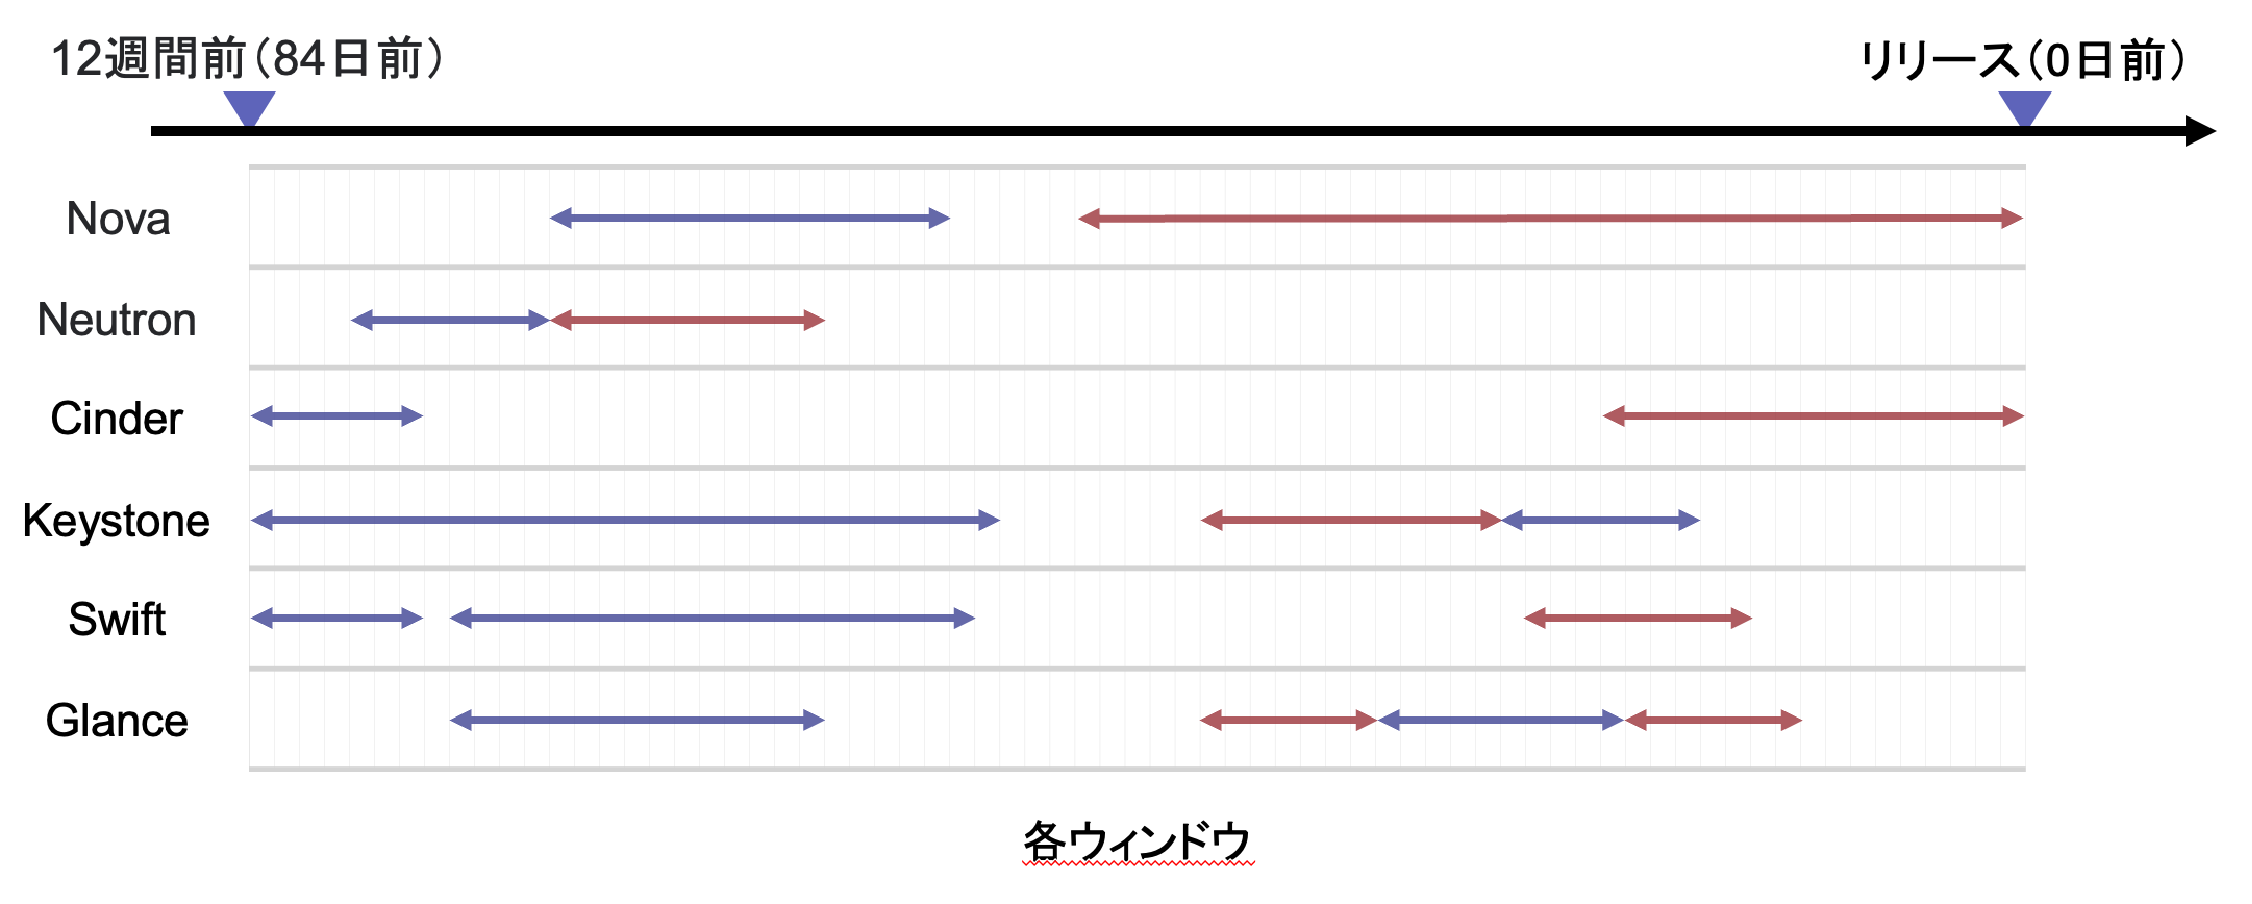
\includegraphics[width=1.0\textwidth]{Uenaka_fig/RQ1_result/merge_f1_window.pdf}
    \caption{導入予測モデルの予測結果:7つ以上の連続したウィンドウにおいて提案モデルのF値がベースラインモデルのF値と比べて向上した(赤)または低下した(青)期間}
    \label{fig:merge_f1_window}
\end{center}
\end{figure}
%-----------------------


\subsubsection{知見4:導入されるチケットの予測において,開発状況を学習することで,Cinder, Swiftプロジェクトでは後期,Keystoneプロジェクトでは中期,Novaプロジェクトでは中期および後期において提案モデルのF値が向上し,Neutronプロジェクトでは前期,Glanceプロジェクトでは中期および後期において提案モデルのF値が向上または低下する}
本知見では,リリース期間を前期(リリースが遠い時)・中期(リリース中頃)・後期(リリースが近い時)の3つに分割し,開発状況の学習有無による導入予測モデルの予測性能が異なるかを明らかにする.図\ref{fig:merge_f1_window}から,前期は1プロジェクト (Neutron) ,中期は3プロジェクト (Nova,Keystone,Glance) ,後期は4プロジェクト (Nova, Cinder, Swift, Glance) において,提案モデルのF値がベースラインモデルのF値と比べて向上するという結果が得られた.また,前期は全てのプロジェクト,後期は2プロジェクト (Keystone, Glance) において,提案モデルのF値がベースラインモデルのF値と比べて低下するという結果が得られた.以下に共通の傾向を持つプロジェクトの結果をまとめる.

\textbf{ (Nova, Cinder, Swift) }後期 (Cinder, Swift) や中期および後期 (Nova) は提案モデルのF値が向上した一方,前期は提案モデルのF値が低下した.よって,これらのプロジェクトでは中期および後期 (Nova) や後期 (Cinder, Swift) において,検証者が導入するチケットが開発状況によって変化していることが示唆される.

\textbf{ (Keystone, Glance) }中期 (Keystone) や中期および後期 (Glance) は提案モデルのF値が向上した一方,前期および後期は提案モデルのF値が低下した.よって,これらのプロジェクトでは中期 (Keystone) や中期および後期の一部の期間 (Glance) において,検証者が導入するチケットが開発状況によって変化していることが示唆される.

\textbf{ (Neutron) }前期は提案モデルのF値が向上または低下した.よって,Neutronプロジェクトでは前期の一部の期間において,検証者が導入するチケットが開発状況によって変化していることが示唆される.

また,適合率および再現率に着目することで,提案モデルでF値が向上した理由を考察する.図\ref{fig:merge_p}および図\ref{fig:merge_r}から,3プロジェクト (Neutron, Keystone, Glance) においては,F値が向上した期間の一部分において適合率も向上したという結果が得られた.また,5プロジェクト (Nova, Neutron, Cinder, Keystone, Swift) においては,F値が向上した期間の一部分において再現率も向上したという結果が得られた.以下に共通の傾向を持つプロジェクトの結果をまとめる.

\textbf{ (Neutron, Keystone) }適合率と再現率の双方が向上したため,開発状況の変化によって検証者が導入するようになるチケットと導入しないようになるチケットが存在し,提案モデルは開発状況を学習することでそれらのチケットを正しく判別したため,F値が向上したと考えられる.

\textbf{ (Glance) }適合率が向上したため,開発状況の変化によって検証者が導入しないようになるチケットが存在し,提案モデルは開発状況を学習することでそれらのチケットを正しく判別したため,F値が向上したと考えられる.

\textbf{ (Nova, Cinder, Swift) }再現率が向上したため,開発状況の変化によって検証者が導入するようになるチケットが存在し,提案モデルは開発状況を学習することでそれらのチケットを正しく判別したため,F値が向上したと考えられる.


%の結果から,Novaプロジェクトでは,ウィンドウ34〜71において提案モデルのF値が0.01〜0.15高くなり,Neutronプロジェクトでは,ウィンドウ13〜23において提案モデルのF値が0.06〜0.22高くなった.図\ref{fig:merge_cinder_keystone}の結果から,Cinderプロジェクトでは,ウィンドウ55〜71において提案モデルのF値が0.04〜0.16高くなり,Keystoneプロジェクトでは,ウィンドウ40〜51において提案モデルのF値が0.06〜0.24高くなった.図\ref{fig:merge_swift_glance}の結果から,Swiftプロジェクトでは,ウィンドウ53〜61において提案モデルのF値が0.01〜0.16高くなり,Glanceプロジェクトでは,ウィンドウ40〜46,56〜62において提案モデルのF値が0.02〜0.18高くなった.これらの結果から,リリースが遠い時はNeutronプロジェクト,リリース中頃はNova,Keystone,Glanceプロジェクト,リリースが近い時はNova,Cinder,Swift,GlanceプロジェクトのF値が向上したため,各プロジェクトはそれぞれのリリースまでの期間において,開発状況によって導入判断が変化することが示唆される.


%-----------------------
\begin{figure}[H]
\begin{minipage}{\textwidth}
\vspace{0.08\textheight}
\begin{center}
    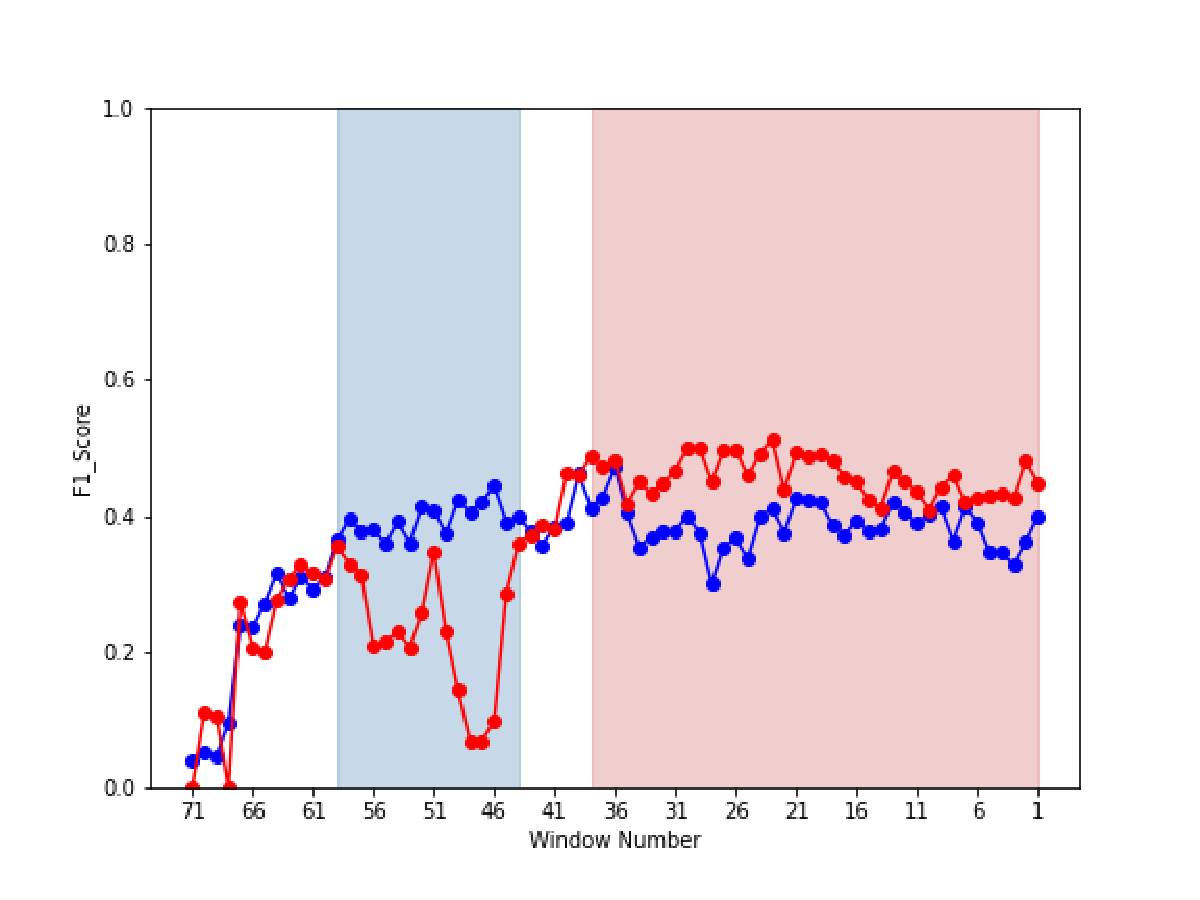
\includegraphics[width=0.495\textwidth]{Uenaka_fig/RQ1_result/Nova_merge_F1.pdf}
    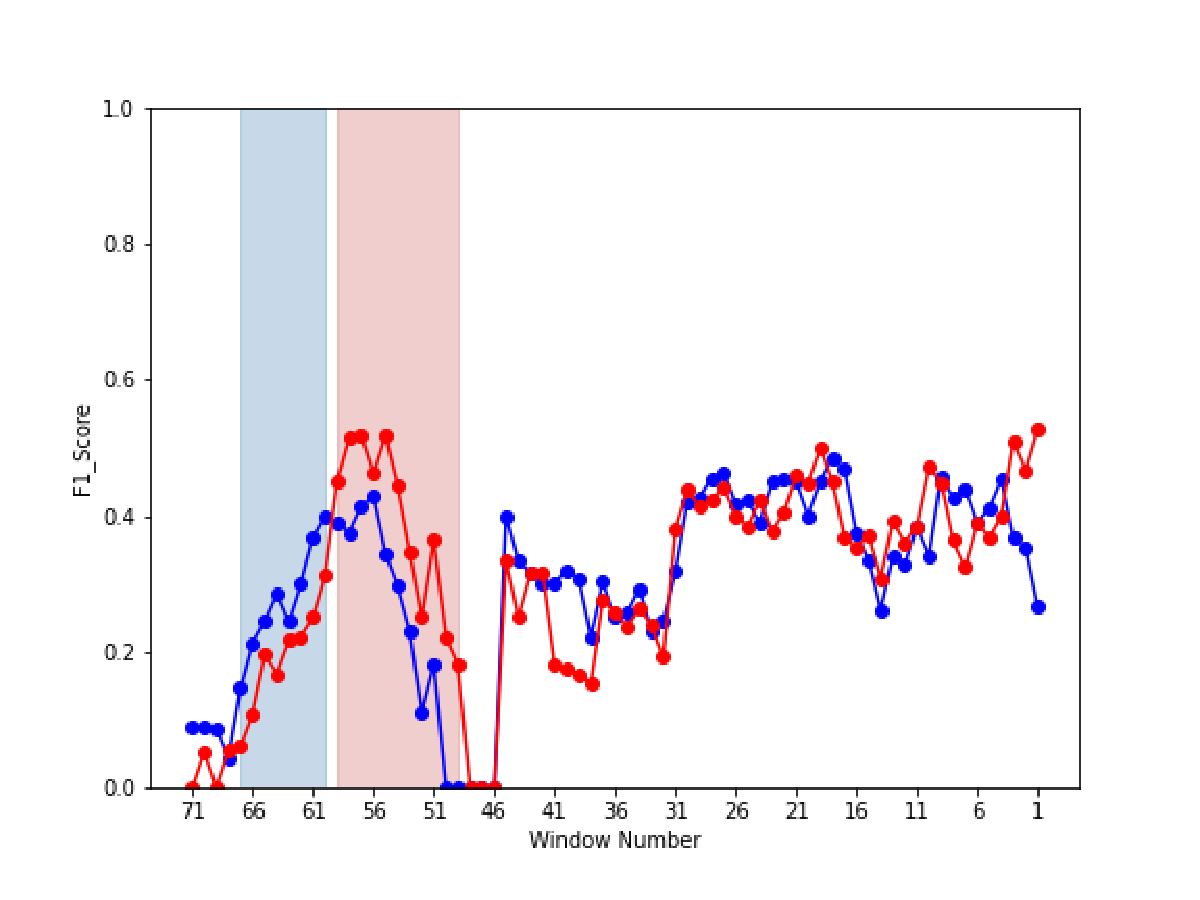
\includegraphics[width=0.495\textwidth]{Uenaka_fig/RQ1_result/Neutron_merge_F1.pdf}
    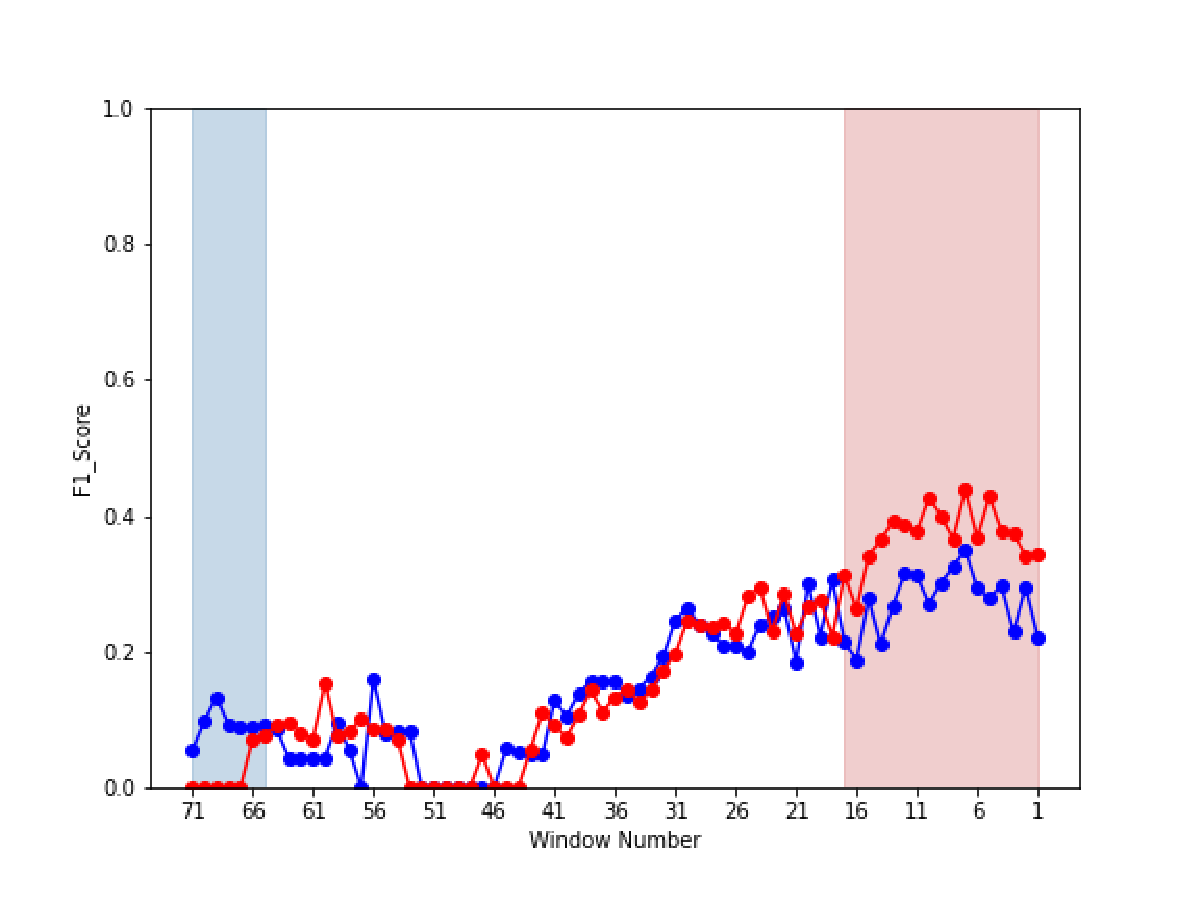
\includegraphics[width=0.495\textwidth]{Uenaka_fig/RQ1_result/Cinder_merge_F1.pdf}
    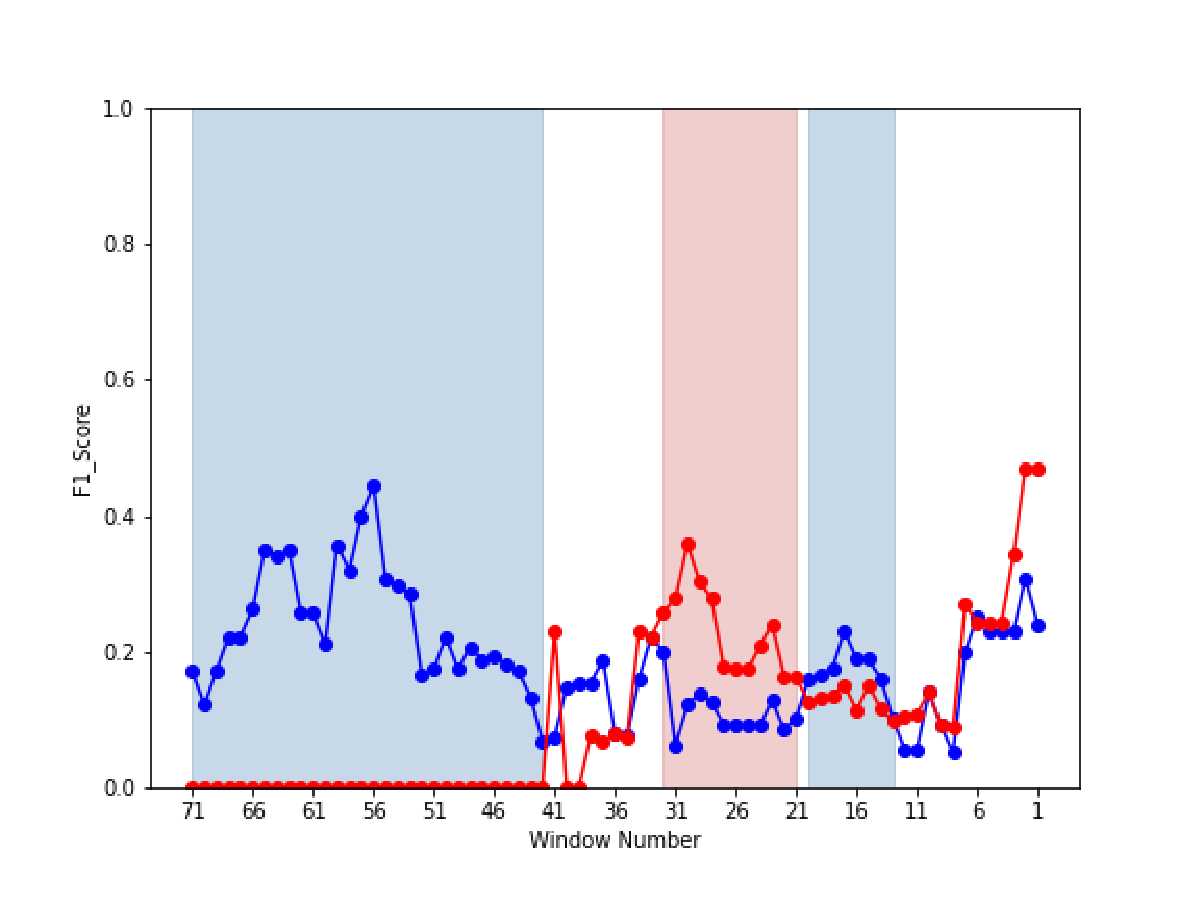
\includegraphics[width=0.495\textwidth]{Uenaka_fig/RQ1_result/Keystone_merge_F1.pdf}
    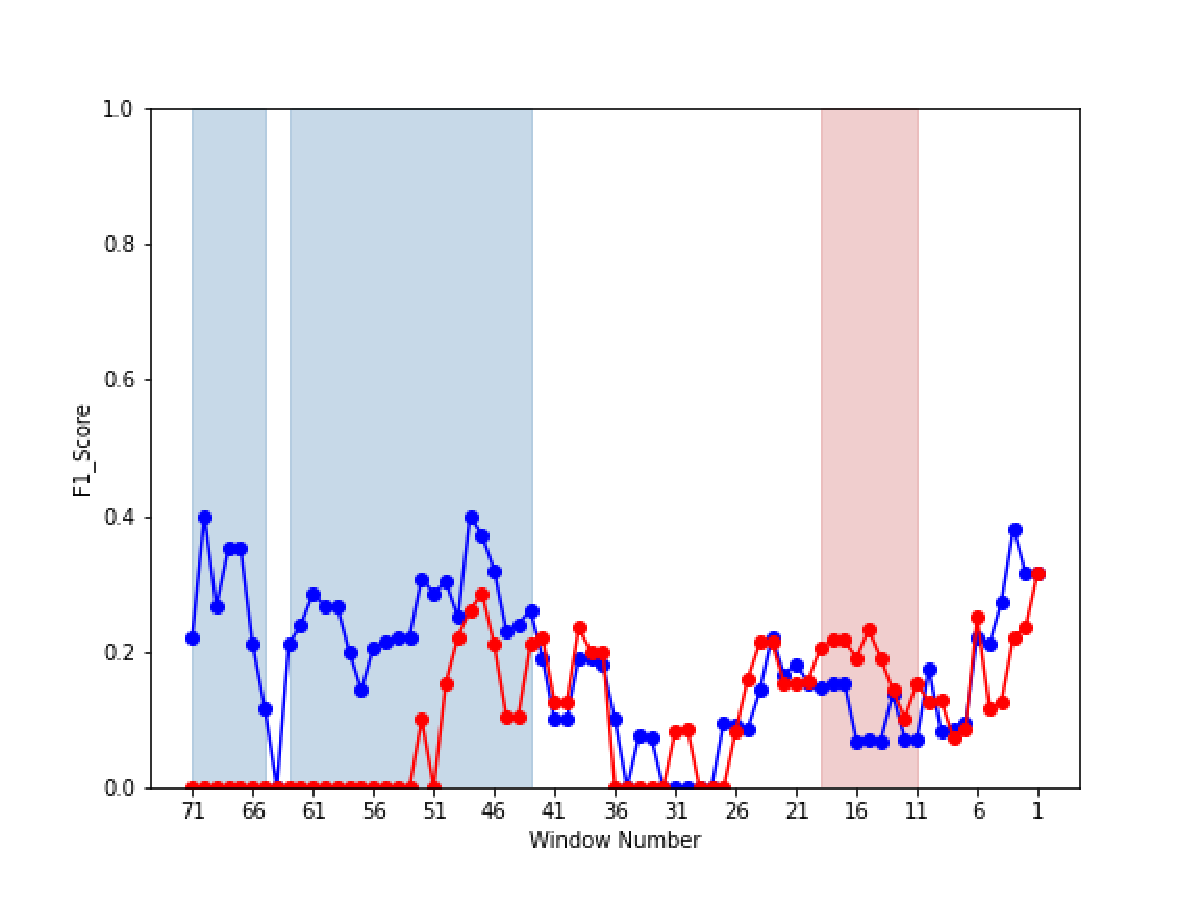
\includegraphics[width=0.495\textwidth]{Uenaka_fig/RQ1_result/Swift_merge_F1.pdf}
    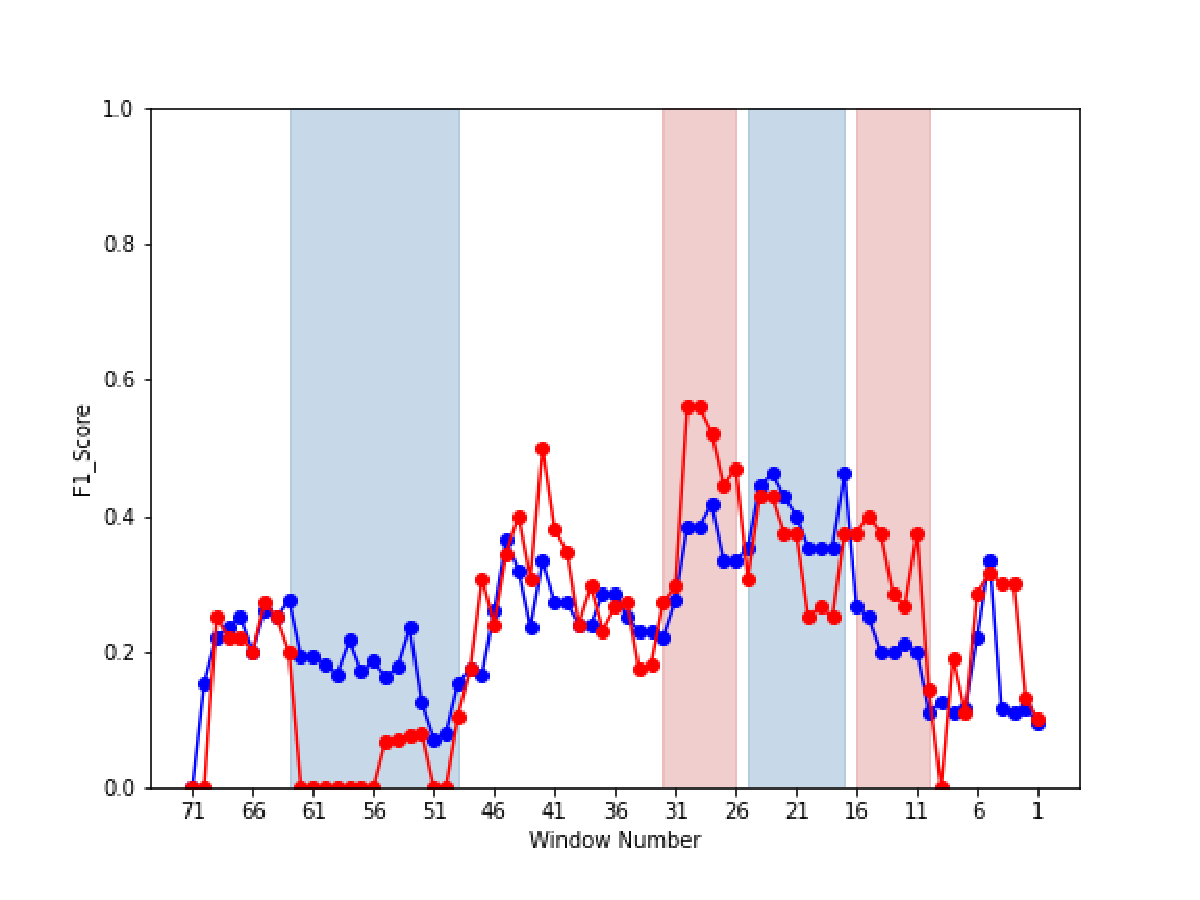
\includegraphics[width=0.495\textwidth]{Uenaka_fig/RQ1_result/Glance_merge_F1.pdf}
    \caption{導入予測モデルのF値(上段左:Nova,上段右:Neutron,中段左:Cinder,\\ 中段右:Keystone,下段左:Swift,下段右:Glance)(赤:提案モデル,青:ベースラインモデル)}
    \label{fig:merge_f}
\end{center}
\vspace{0.08\textheight}
\end{minipage}
\end{figure}
%-----------------------

%-----------------------
\begin{figure}[H]
\begin{minipage}{\textwidth}
\vspace{0.08\textheight}
\begin{center}
    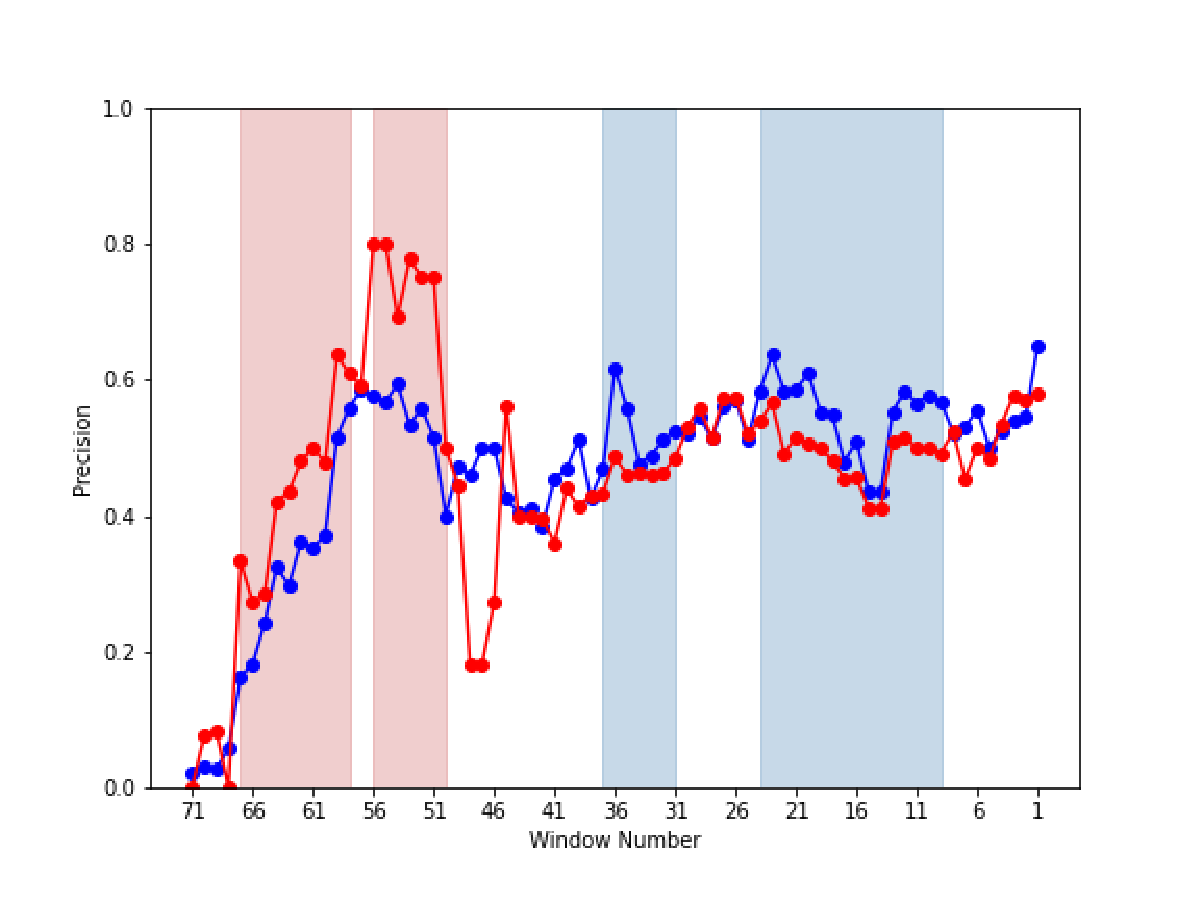
\includegraphics[width=0.495\textwidth]{Uenaka_fig/RQ1_result/Nova_merge_Precision.pdf}
    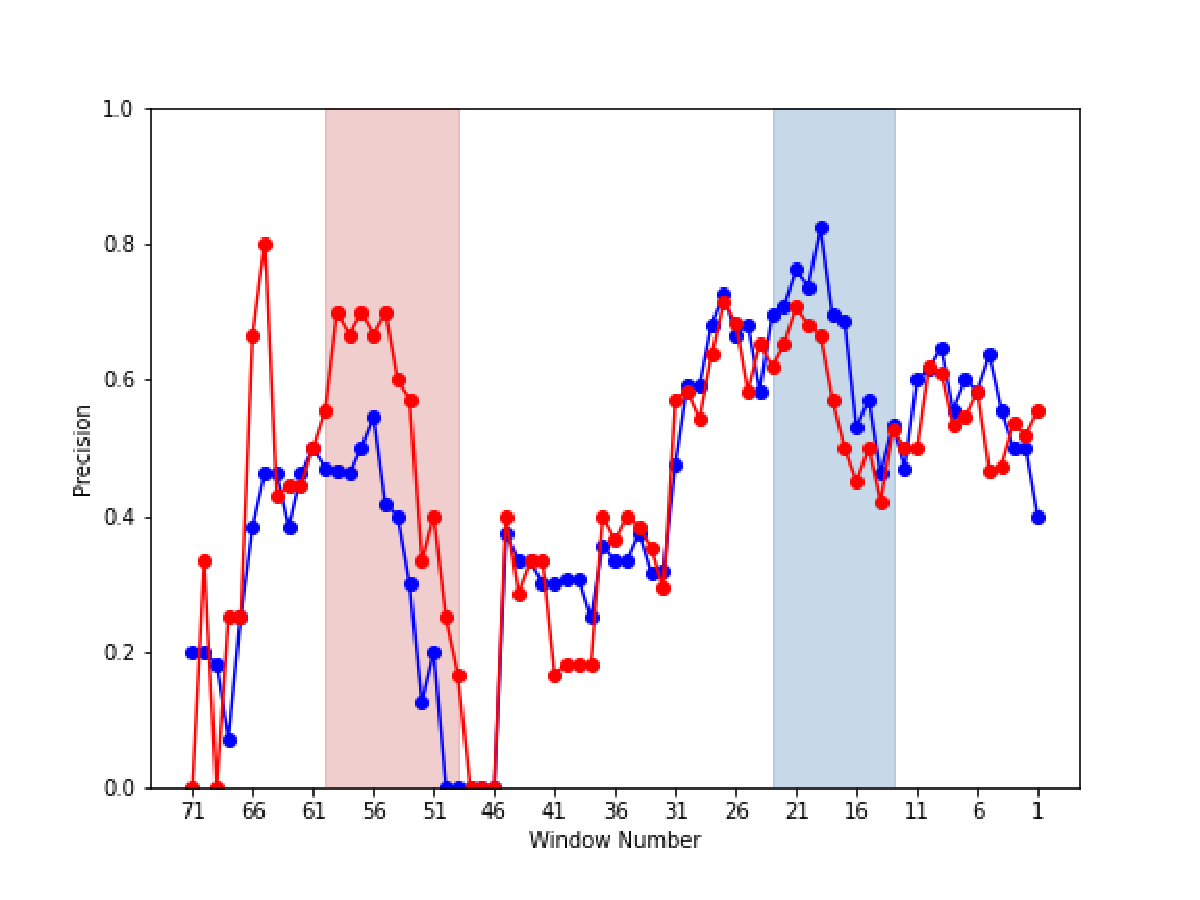
\includegraphics[width=0.495\textwidth]{Uenaka_fig/RQ1_result/Neutron_merge_Precision.pdf}
    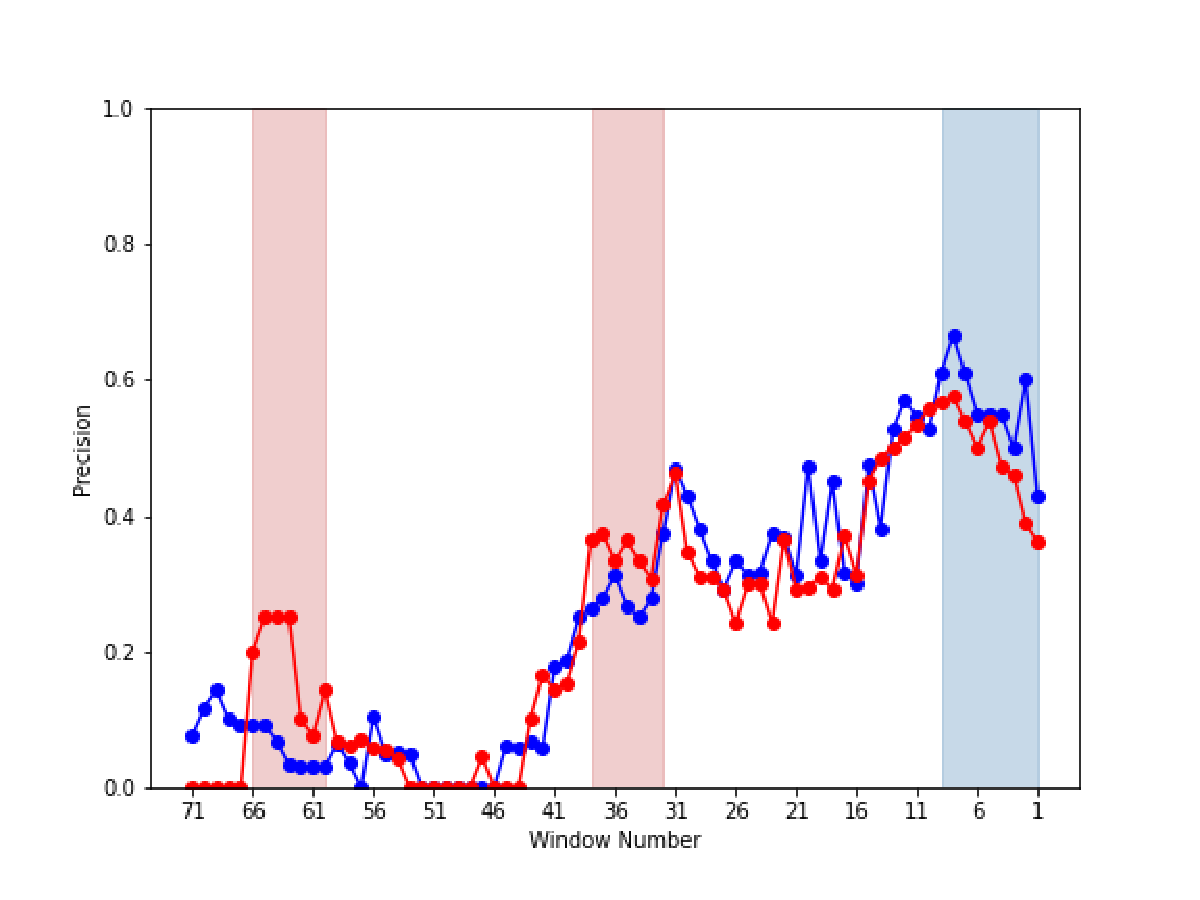
\includegraphics[width=0.495\textwidth]{Uenaka_fig/RQ1_result/Cinder_merge_Precision.pdf}
    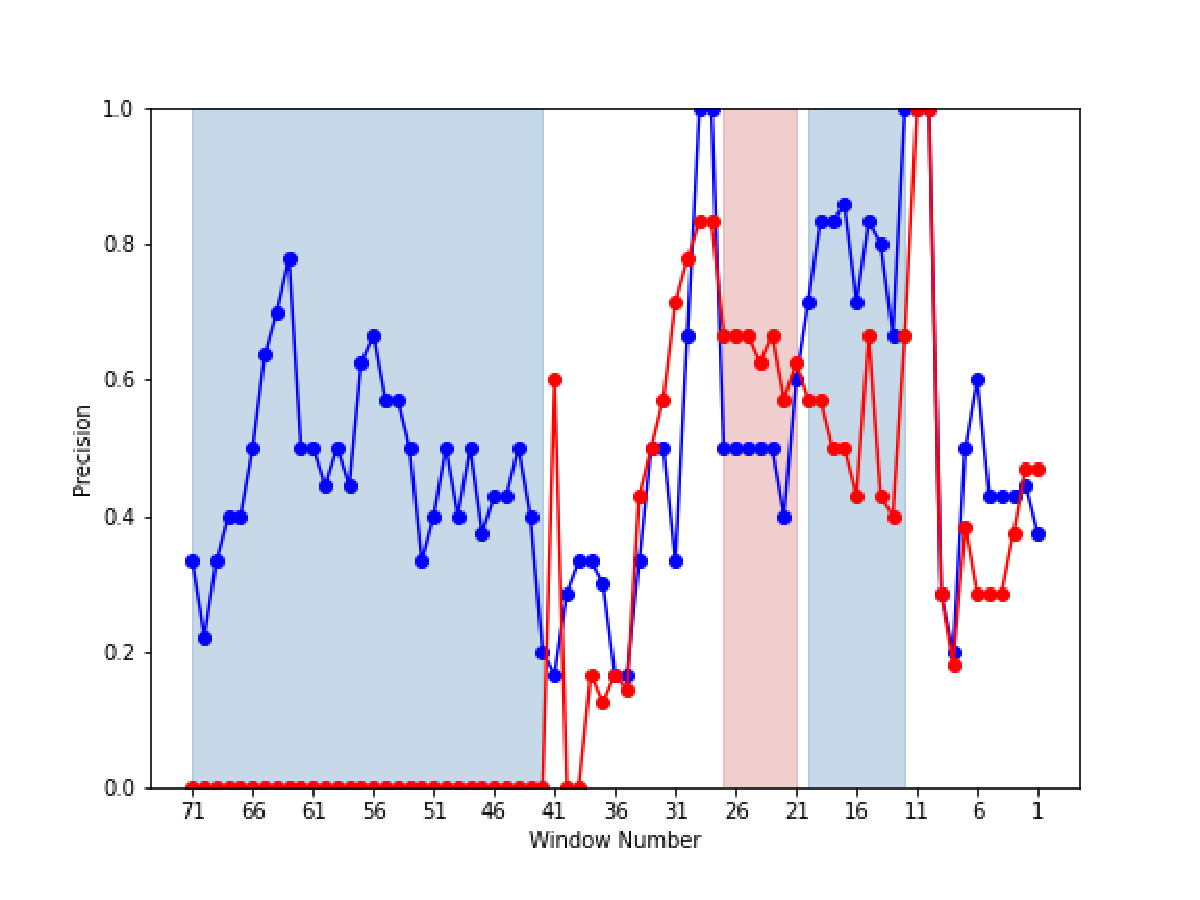
\includegraphics[width=0.495\textwidth]{Uenaka_fig/RQ1_result/Keystone_merge_Precision.pdf}
    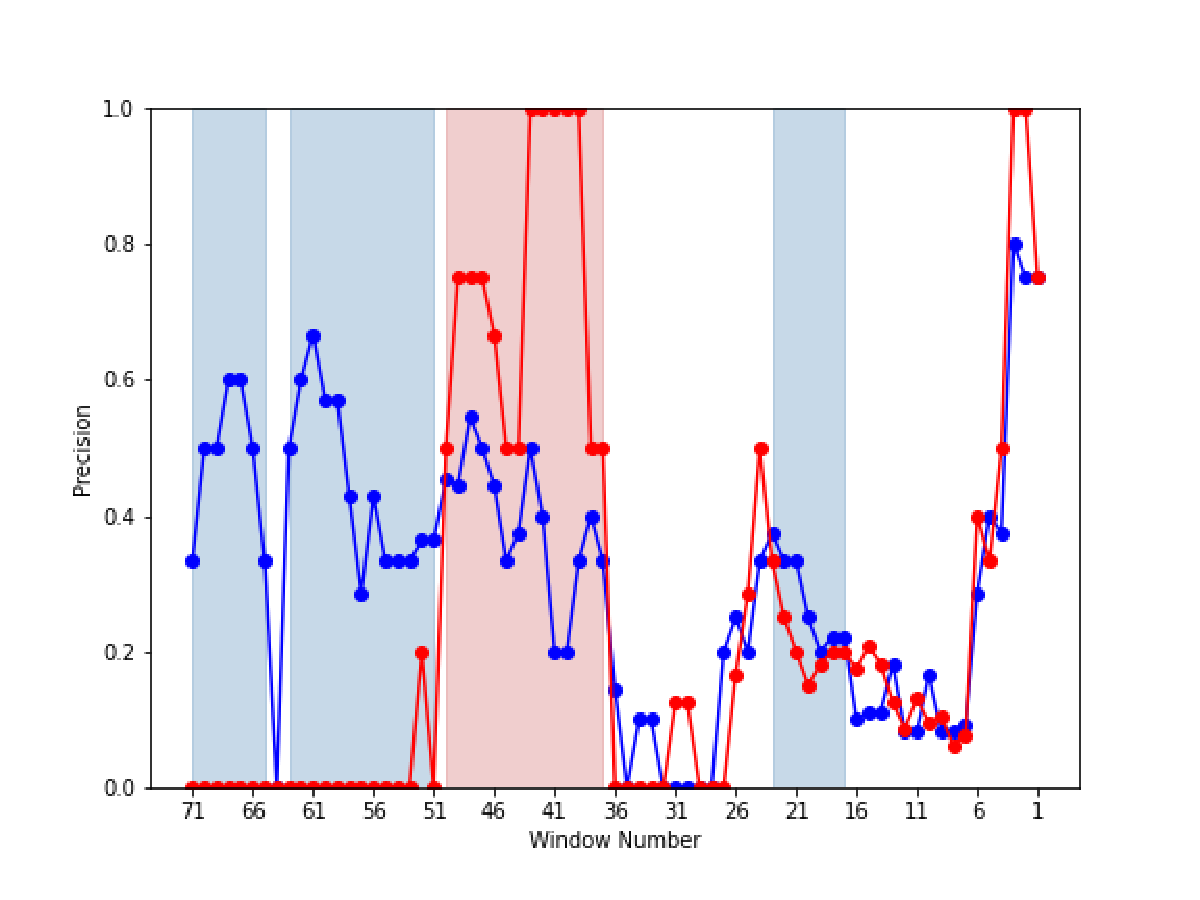
\includegraphics[width=0.495\textwidth]{Uenaka_fig/RQ1_result/Swift_merge_Precision.pdf}
    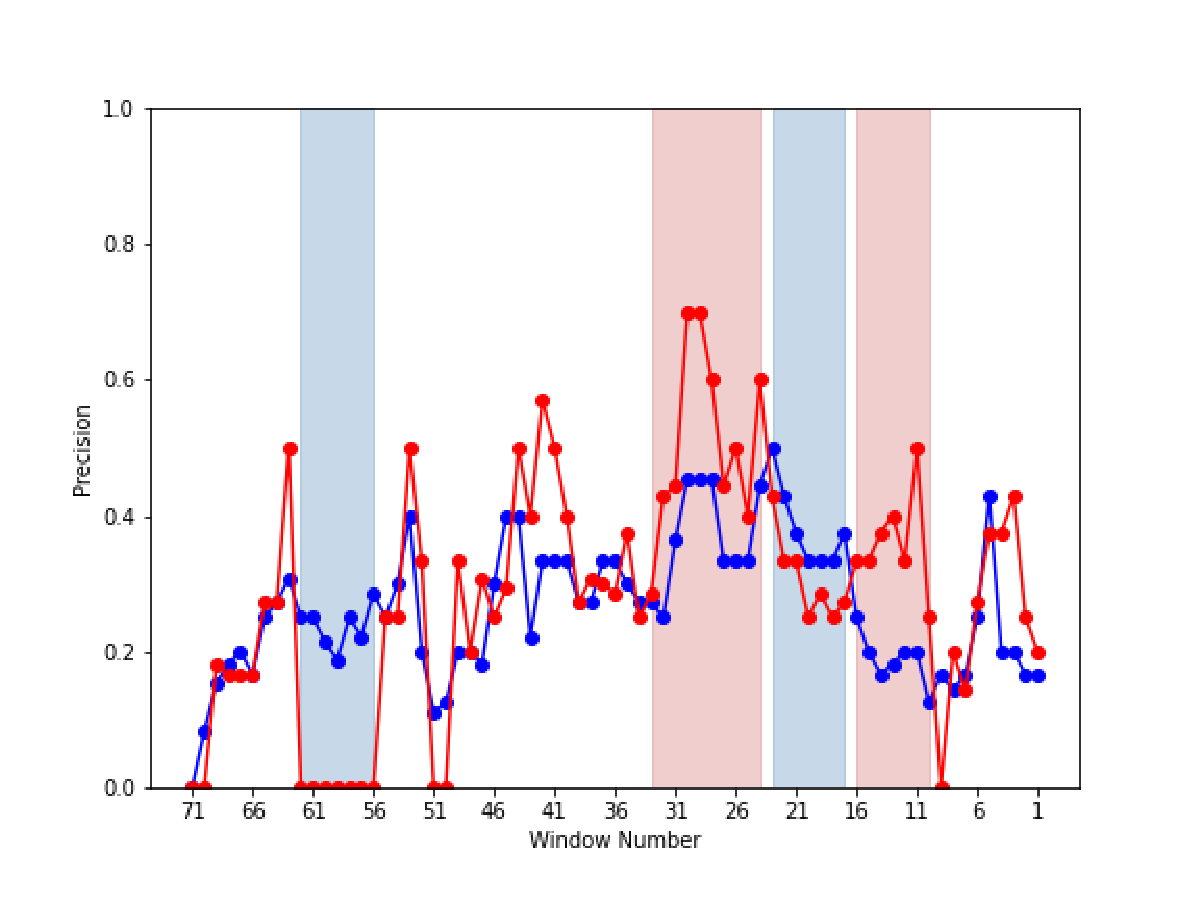
\includegraphics[width=0.495\textwidth]{Uenaka_fig/RQ1_result/Glance_merge_Precision.pdf}
    \caption{導入予測モデルの適合率(上段左:Nova,上段右:Neutron,中段左:Cinder,\\ 中段右:Keystone,下段左:Swift,下段右:Glance)(赤:提案モデル,青:ベースラインモデル)}
    \label{fig:merge_p}
\end{center}
\vspace{0.08\textheight}
\end{minipage}
\end{figure}
%-----------------------

%-----------------------
\begin{figure}[H]
\begin{minipage}{\textwidth}
\vspace{0.08\textheight}
\begin{center}
    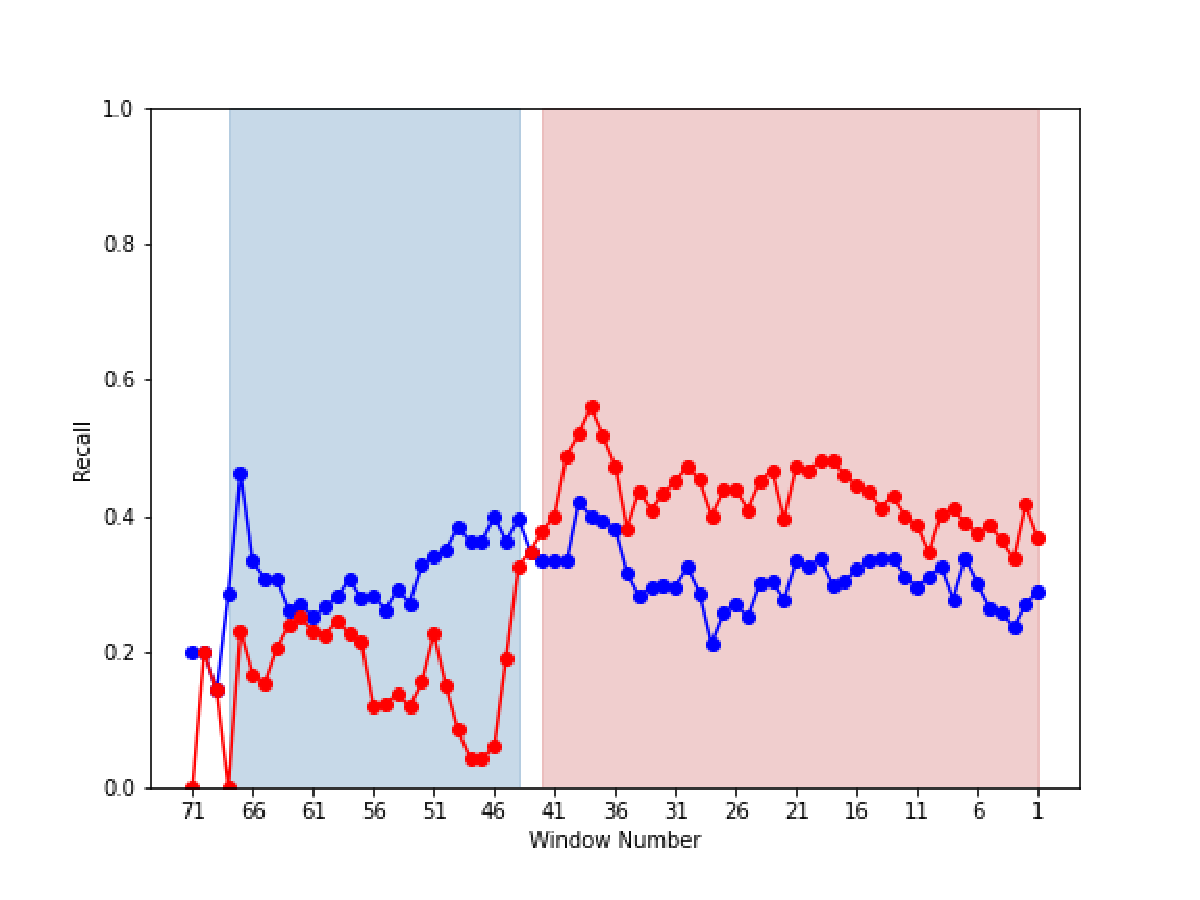
\includegraphics[width=0.495\textwidth]{Uenaka_fig/RQ1_result/Nova_merge_Recall.pdf}
    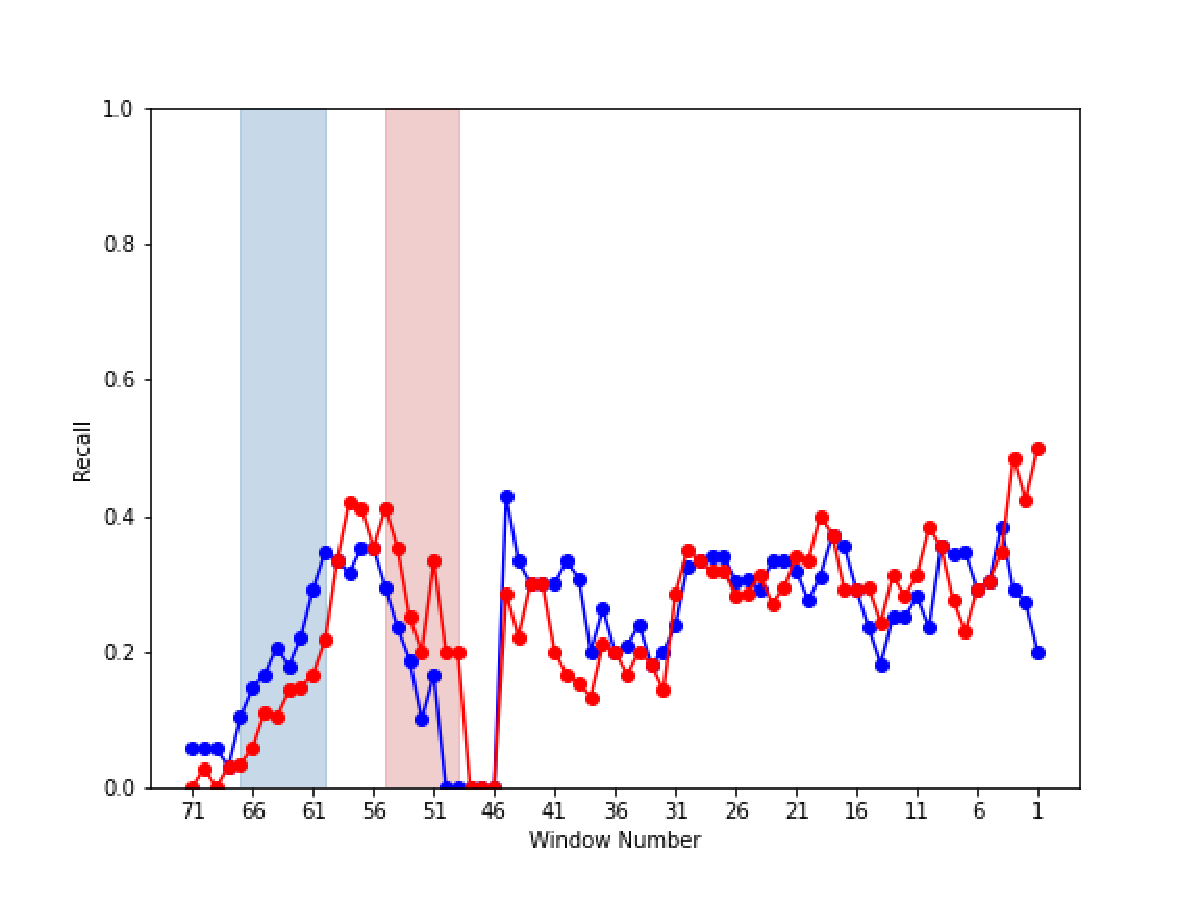
\includegraphics[width=0.495\textwidth]{Uenaka_fig/RQ1_result/Neutron_merge_Recall.pdf}
    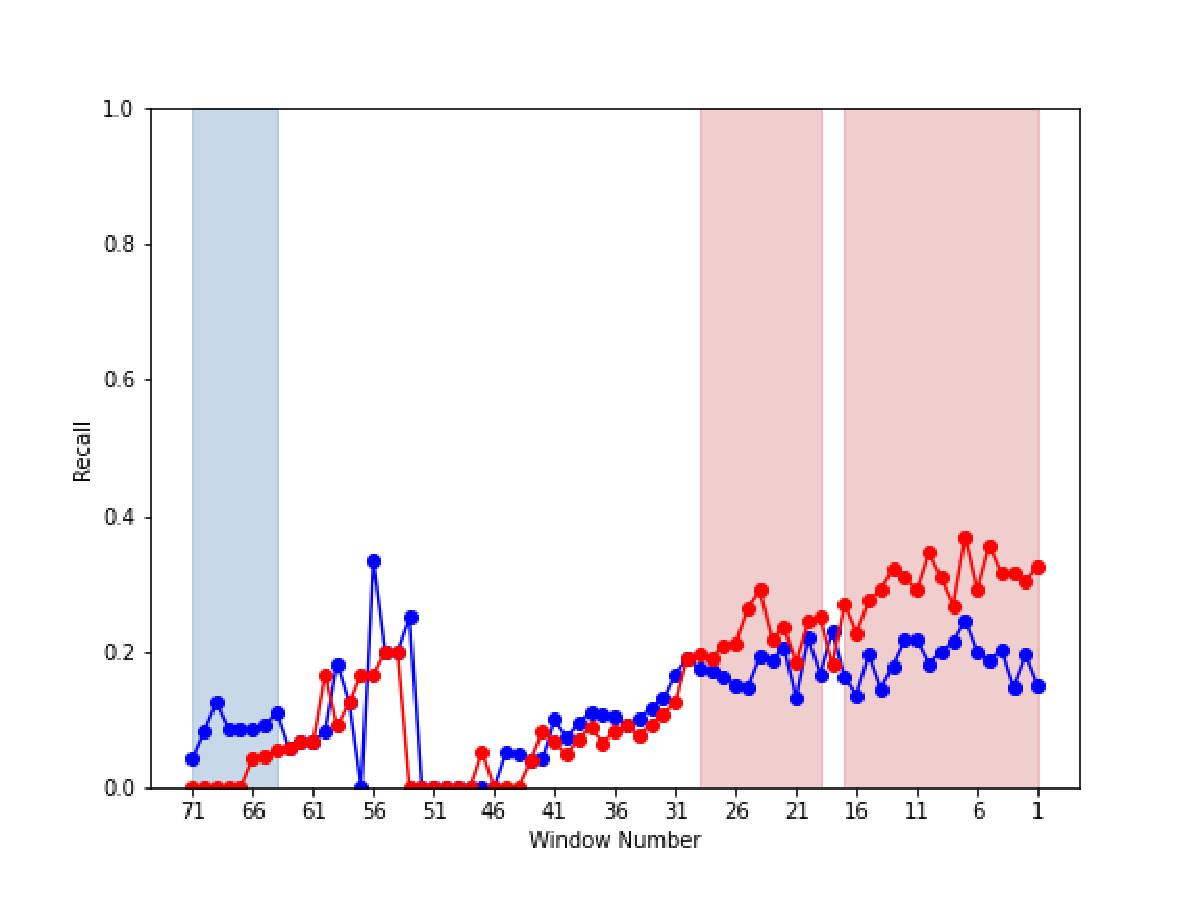
\includegraphics[width=0.495\textwidth]{Uenaka_fig/RQ1_result/Cinder_merge_Recall.pdf}
    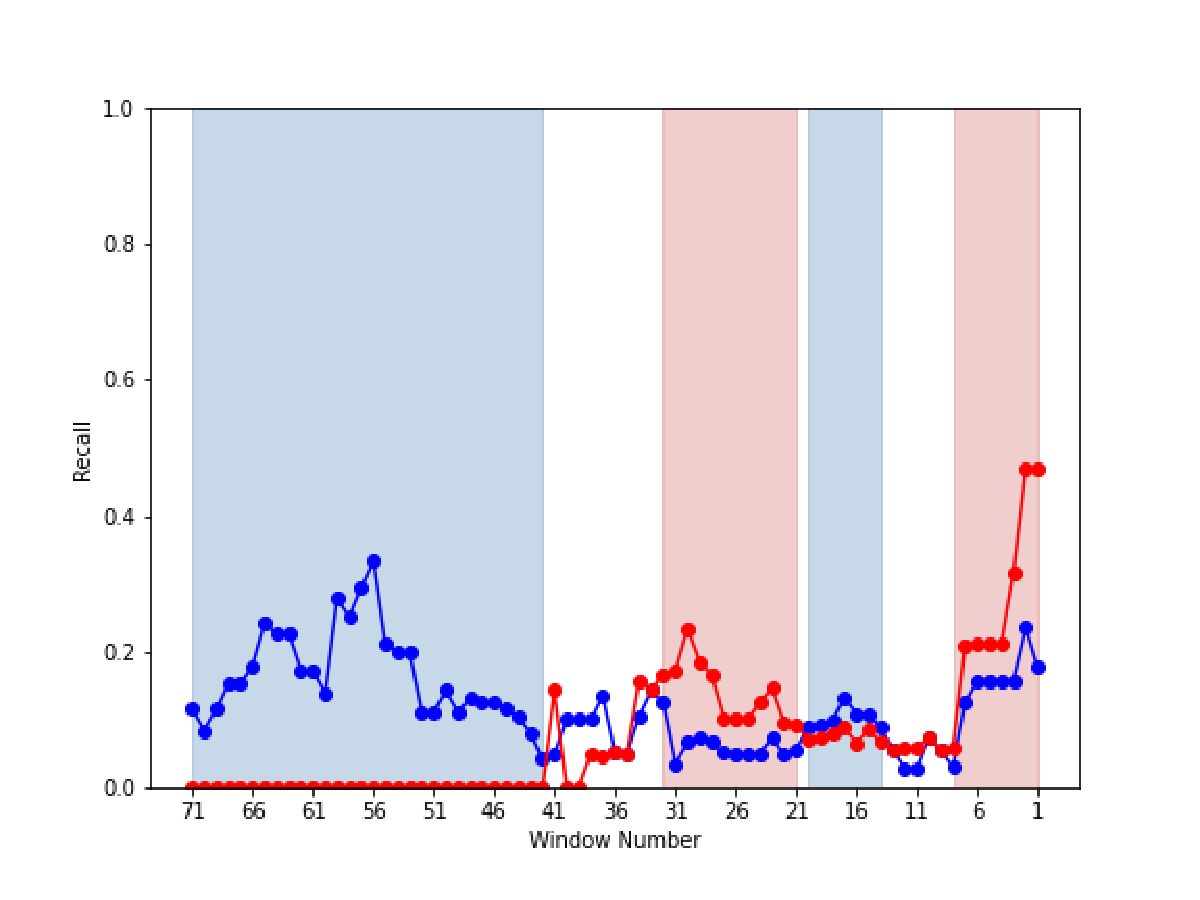
\includegraphics[width=0.495\textwidth]{Uenaka_fig/RQ1_result/Keystone_merge_Recall.pdf}
    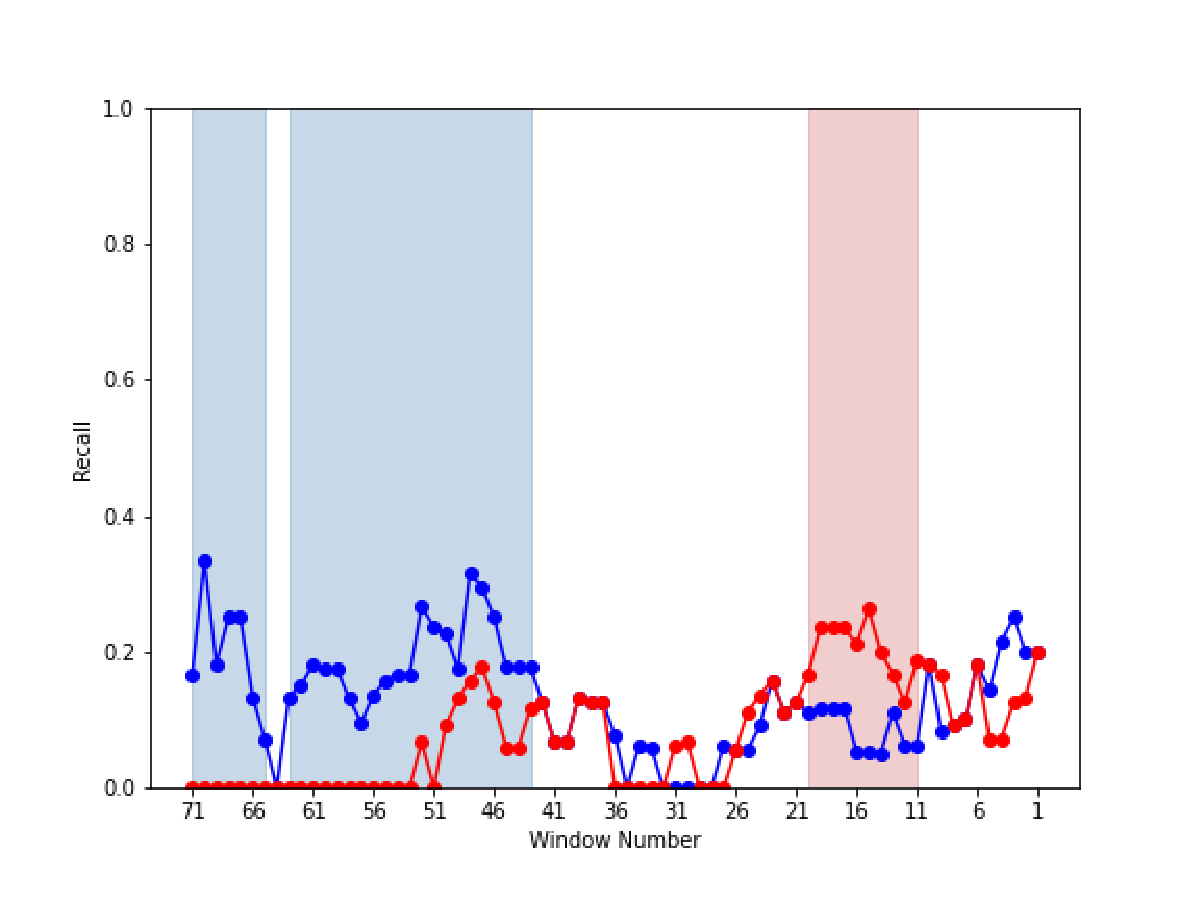
\includegraphics[width=0.495\textwidth]{Uenaka_fig/RQ1_result/Swift_merge_Recall.pdf}
    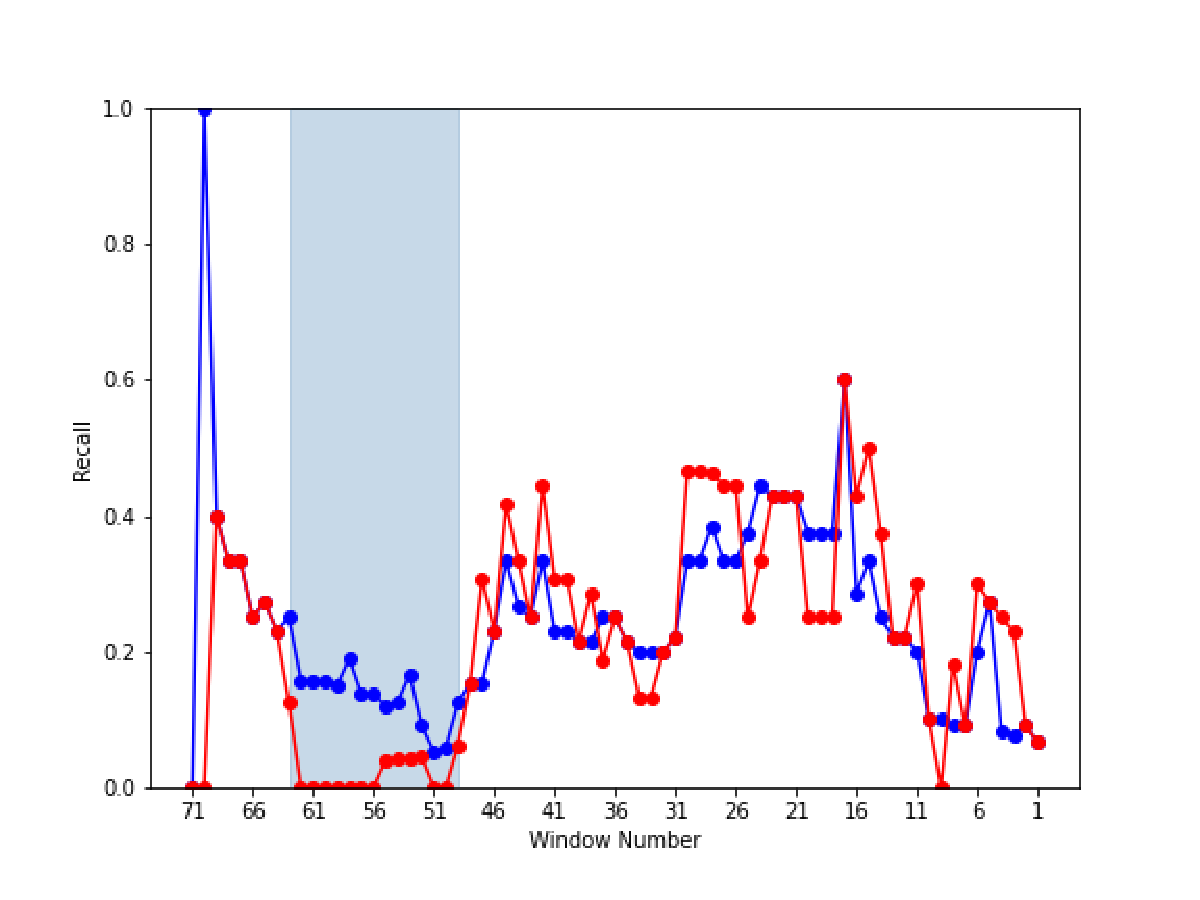
\includegraphics[width=0.495\textwidth]{Uenaka_fig/RQ1_result/Glance_merge_Recall.pdf}
    \caption{導入予測モデルの再現率(上段左:Nova,上段右:Neutron,中段左:Cinder,\\ 中段右:Keystone,下段左:Swift,下段右:Glance)(赤:提案モデル,青:ベースラインモデル)}
    \label{fig:merge_r}
\end{center}
\vspace{0.08\textheight}
\end{minipage}
\end{figure}
%-----------------------


%%%%%%%%%%%%%%%%%%%%%%%%%%%%%%%%%
\chapter{RQ2:\rqtwo}\label{sec:rq2}
%%%%%%%%%%%%%%%%%%%%%%%%%%%%%%%%%
RQ2では,ベースラインモデルの再現率(正例の網羅率)および特異度(負例の網羅率)のリリース期間内での変化を,\ref{sec:rq1}章と同様に回帰係数を用いて分析することで,各プロジェクトにおいてチケットおよびチケット実装者の特徴から正しく判別できるチケットの割合がリリースまでの期間内でどのように変化するかを明らかにする.
次に,提案モデルとベースラインモデルの再現率および特異度を比較し,提案モデルの網羅率がベースラインモデルの網羅率より高くなる期間を明らかにすることで,開発状況によって検証者の検証判断/導入判断が一部のチケットで変化する期間および判断の変化を考察する.

\section{分析結果}
\subsection{検証予測モデル}
検証予測モデルの予測結果として,図\ref{fig:review_spec}は各プロジェクトの特異度を示す.図は縦軸が特異度を表し,横軸や折れ線,図の配置や色で表されている期間の定義は\ref{sec:rq1_kenshou}項と同様である.特異度および再現率についてまとめたものを図\ref{fig:review_sperec_window}に示す.
また,表\ref{table:review_spec_jikeiretsu}はベースラインモデルの再現率および特異度の時系列変化の分析結果として,各プロジェクトの検証予測モデルにおける再現率および特異度の回帰係数の分類を示す.表\ref{table:review_spec_jikeiretsu}において,回帰係数の分類は表\ref{table:review_seino_jikeiretsu}と同様の矢印で表す.

\subsubsection{知見1:2プロジェクト (Nova, Keystone) ではリリースが近づくにつれてチケットおよびチケット実装者の特徴に基づいて検証を開始しないチケットを判断し,2プロジェクト (Neutron, Cinder) ではチケットおよびチケット実装者の特徴以外の要因に基づき,2プロジェクト (Swift, Glance) では判断の割合が変化しない}
本知見では,チケットおよびチケット実装者の特徴から,チケットに対する検証判断を正しく判別できるチケットの割合がリリースまでの期間内でどのように変化するかを明らかにする.表\ref{table:review_spec_jikeiretsu}の回帰係数の分類から,ベースラインモデルの特異度は2プロジェクト (Nova, Keystone) において回帰係数が有意に増加し,2プロジェクト (Neutron, Cinder) において回帰係数が有意に減少し,2プロジェクト (Swift, Glance) において回帰係数が有意に増加および減少しないという結果が得られた.また,ベースラインモデルの再現率は3プロジェクト (Nova, Cinder, Glance) において回帰係数が有意に増加し,3プロジェクト (Neutron, Keystone, Swift) において回帰係数が有意に増加および減少しないという結果が得られた.以下に共通の傾向を持つプロジェクトの結果をまとめる.

\textbf{ (Nova, Keystone) }リリースが近づくにつれて,チケットおよびチケット実装者の特徴から正しく負例と判別できるチケットの割合が増加し,正しく正例と判別できるチケットの割合は増加する (Nova) ,リリース期間全体を通して概ね一定である (Keystone) ことを明らかにした.この結果から,当該プロジェクトの検証者はリリースが近づくにつれて,チケットおよびチケット実装者の特徴に基づいて検証を開始しないチケットを判断するようになることが示唆される.

\textbf{ (Neutron, Cinder) }リリースが近づくにつれて,チケットおよびチケット実装者の特徴から正しく負例と判別できるチケットの割合が減少し,正しく正例と判別できるチケットの割合は増加する (Cinder) ,リリース期間全体を通して概ね一定である (Neutron) ことを明らかにした.この結果から,当該プロジェクトの検証者はリリースが近づくにつれて,チケットおよびチケット実装者の特徴以外の要因に基づいて検証を開始しないチケットを判断するようになることが示唆される.

\textbf{ (Swift, Glance) }リリース期間全体を通して,チケットおよびチケット実装者の特徴から正しく負例と判別できるチケットの割合が概ね一定であり,リリースが近づくにつれて,正しく正例と判別できるチケットの割合は増加する (Glance) ,リリース期間全体を通して概ね一定である (Swift) ことを明らかにした.この結果から,当該プロジェクトの検証者はリリース期間全体を通して,チケットおよびチケット実装者の特徴に基づいて検証を開始しないチケットを判断する割合が変化しないことが示唆される.

%--------------------
\begin{table*}[t]
\caption{各プロジェクトの検証予測モデルにおける再現率(再掲),特異度の回帰係数の分類}
\label{table:review_spec_jikeiretsu}
\centering
\vspace{0.5zh}
\scalebox{0.9}{
\begin{tabular}{l|c|c|c|c|c|c}
    \hline \hline
    評価指標 & Nova & Neutron & Cinder & Keystone & Swift & Glance \\ \hline
    再現率 & $\nearrow$ & $\rightarrow$ & $\nearrow$ & $\rightarrow$ & $\rightarrow$ & $\nearrow$ \\ \hline
    特異度 & $\nearrow$ & $\searrow$ & $\searrow$ & $\nearrow$ & $\rightarrow$ & $\rightarrow$ \\ \hline
\end{tabular}}
\end{table*}
%--------------------

\subsubsection{知見2:開発状況によって検証者の検証判断が一部のチケットで変化する期間および判断の変化は,プロジェクトによって異なる}
本知見では,リリース期間を前期(リリースが遠い時)・中期(リリース中頃)・後期(リリースが近い時)の3つに分割し,開発状況によって検証者の検証判断が一部のチケットで変化する期間および判断の変化を明らかにする.図\ref{fig:review_sperec_window}の結果から,\ref{sec:ticket_tokutei}節の解釈に従ってプロジェクトごとの傾向をまとめる.

\textbf{ (Nova) }リリース期間全体を通して,一部のチケットは開発状況によって検証者が検証を開始しないようになり,前期の一部のチケットは,開発状況によって検証者が検証を開始するようになることが示唆される.

\textbf{ (Neutron) }後期の一部のチケットは,開発状況によって検証者が検証を開始しないようになることが示唆される.

\textbf{ (Cinder) }前期および中期の一部のチケットは,開発状況によって検証者が検証を開始するようになり,前期の一部のチケットは,開発状況によって検証者が検証を開始しないようになることが示唆される.

\textbf{ (Keystone) }中期および後期の一部のチケットは,開発状況によって検証者が検証を開始しないようになることが示唆される.

\textbf{ (Swift) }前期および中期の一部のチケットは,開発状況によって検証者が検証を開始しないようになり,後期の一部のチケットは,開発状況によって検証者が検証を開始するようになることが示唆される.

\textbf{ (Glance) }前期の一部のチケットは,開発状況によって検証者が検証を開始するもしくは開始しないようになり,中期の一部のチケットは,開発状況によって検証者が検証を開始するようになることが示唆される.

%リリースが遠い時は3プロジェクト (Nova, Cinder, Glance) ,リリース中頃は2プロジェクト (Cinder, Glance) ,リリースが近い時は1プロジェクト (Swift) において,提案モデルの再現率がベースラインモデルの再現率と比べて向上するという結果が得られた.また,リリースが遠い時は3プロジェクト (Neutron, Keystone, Swift) ,リリース中頃は2プロジェクト (Neutron, Swift) ,リリースが近い時は3プロジェクト (Neutron, Keystone, Glance) において,提案モデルの再現率がベースラインモデルの再現率と比べて低下するという結果が得られた.また,図\ref{fig:review_spec}から,リリースが遠い時は4プロジェクト (Nova,Cinder,Swift,Glance) ,リリース中頃は3プロジェクト (Nova, Keystone, Swift) ,リリースが近い時は3プロジェクト (Nova, Neutron, Keystone) において,提案モデルの特異度がベースラインモデルの特異度と比べて向上するという結果が得られた.また,リリース中頃は2プロジェクト (Cinder, Glance) ,リリースが近い時は3プロジェクト (Neutron, Swift, Glance) において,提案モデルの特異度がベースラインモデルの特異度と比べて低下するという結果が得られた.


%-----------------------
\begin{figure}[t]
\begin{center}
    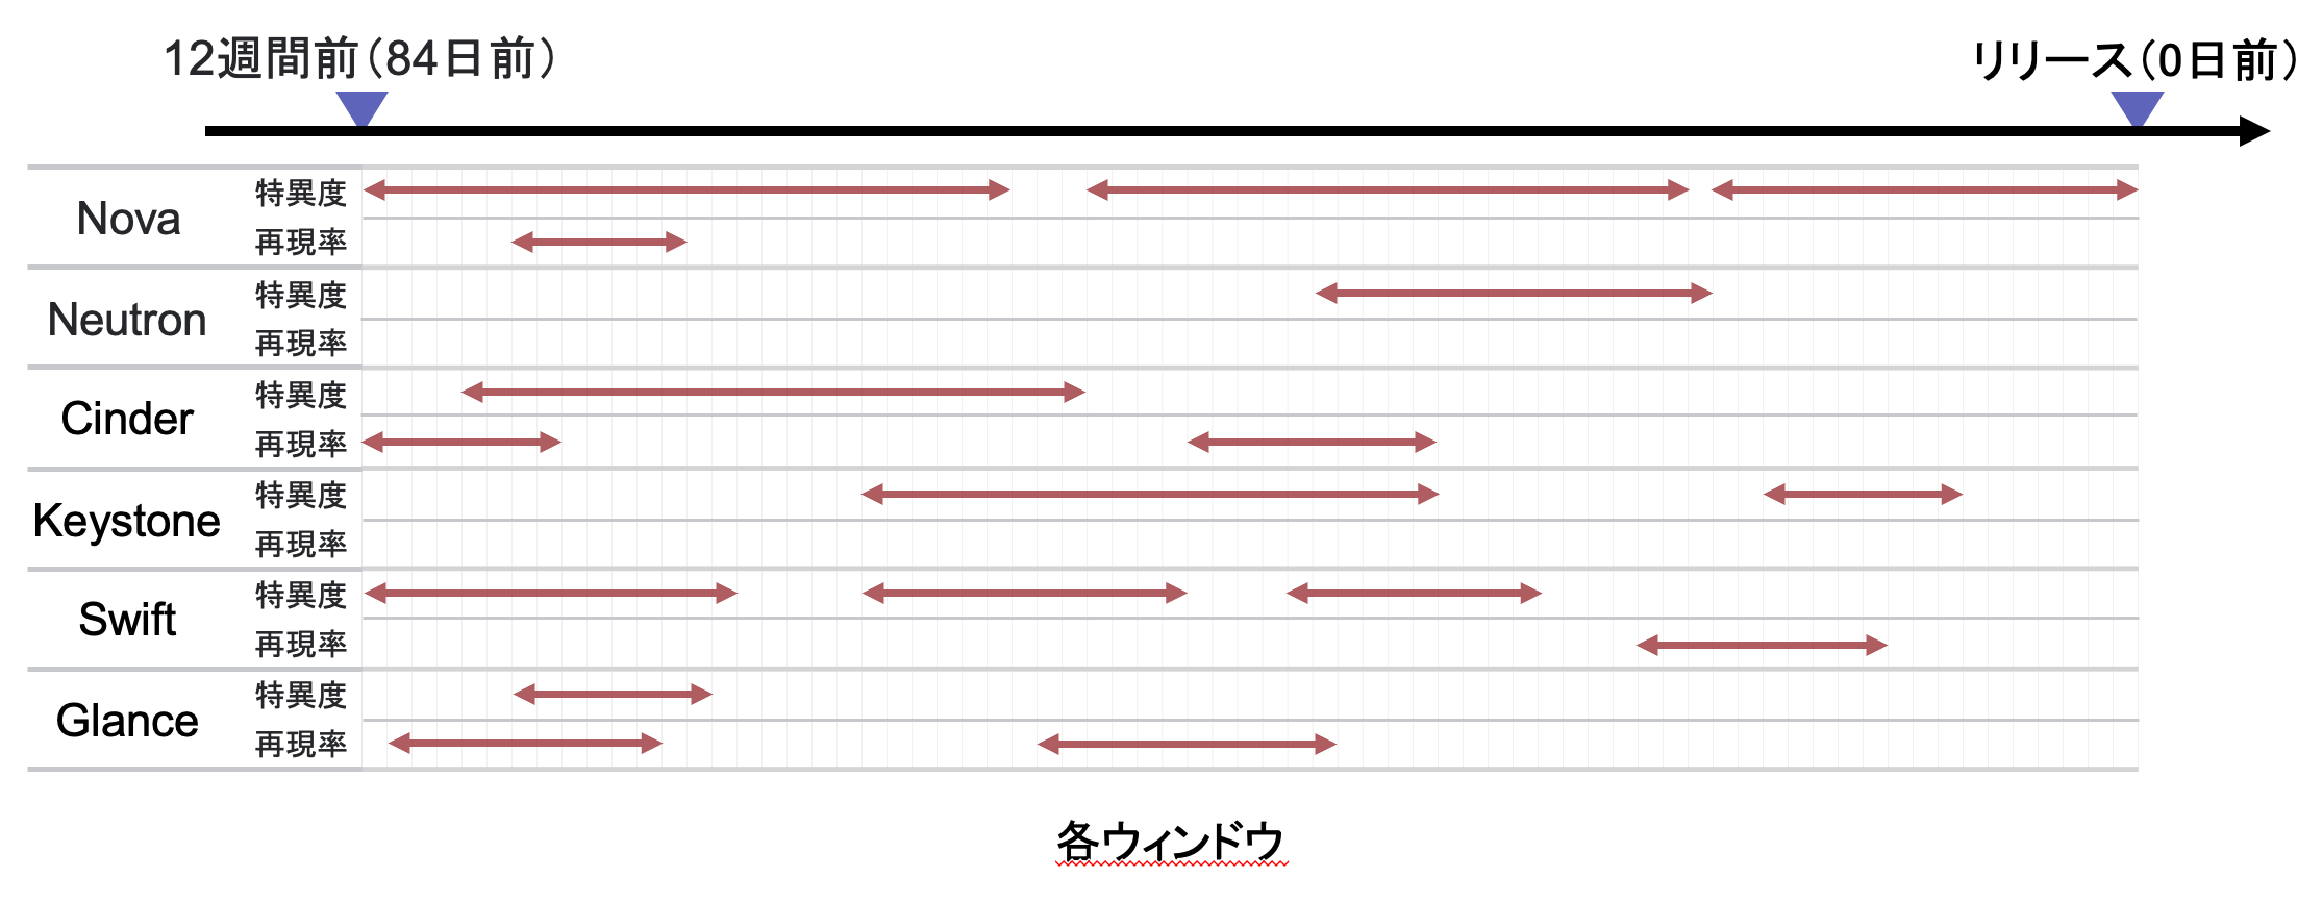
\includegraphics[width=1.0\textwidth]{Uenaka_fig/RQ2_result/review_sperec_window.pdf}
    \caption{検証予測モデルの予測結果:7つ以上の連続したウィンドウにおいて提案モデルの特異度,再現率がベースラインモデルの特異度,再現率と比べて向上した期間}
    \label{fig:review_sperec_window}
\end{center}
\end{figure}
%-----------------------



%-----------------------
\begin{figure}[H]
\begin{center}
    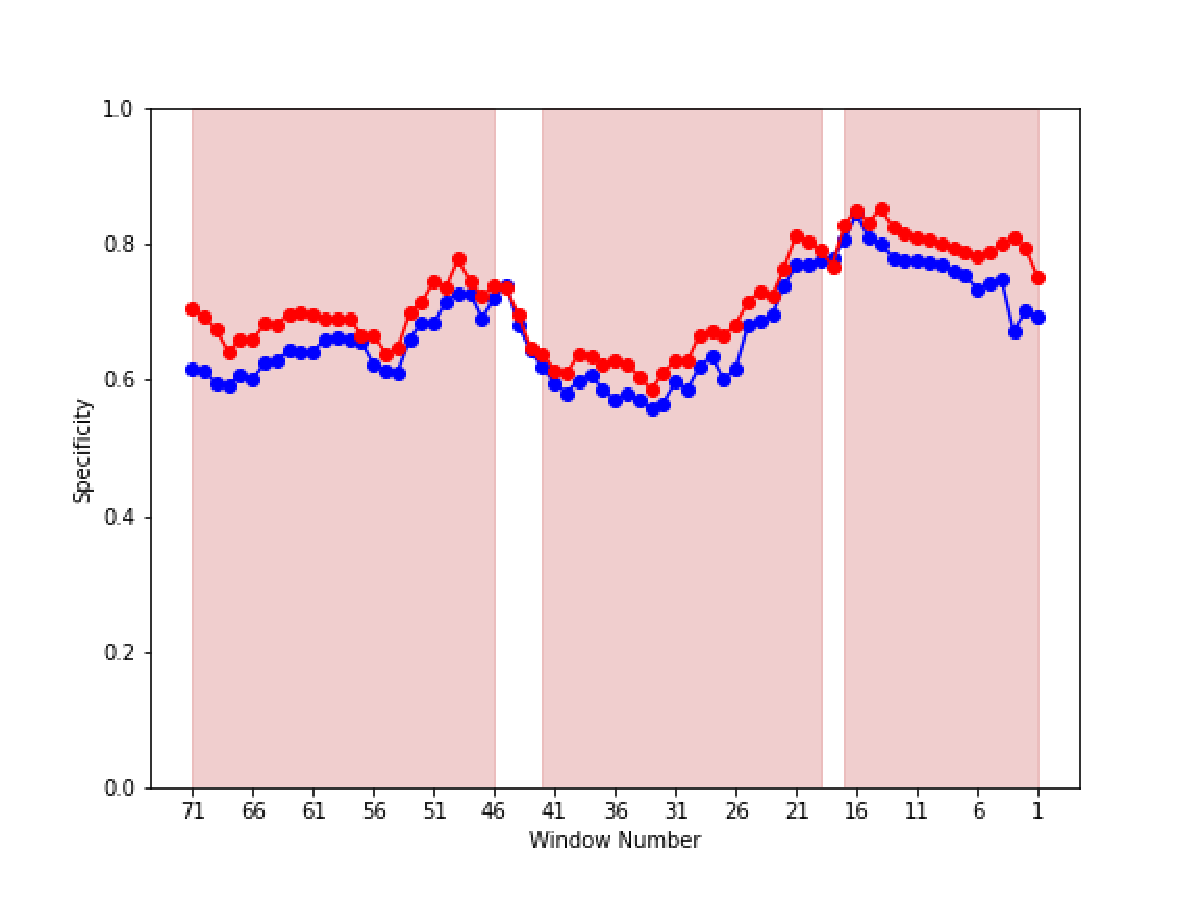
\includegraphics[width=0.495\textwidth]{Uenaka_fig/RQ2_result/Nova_review_Specificity.pdf}
    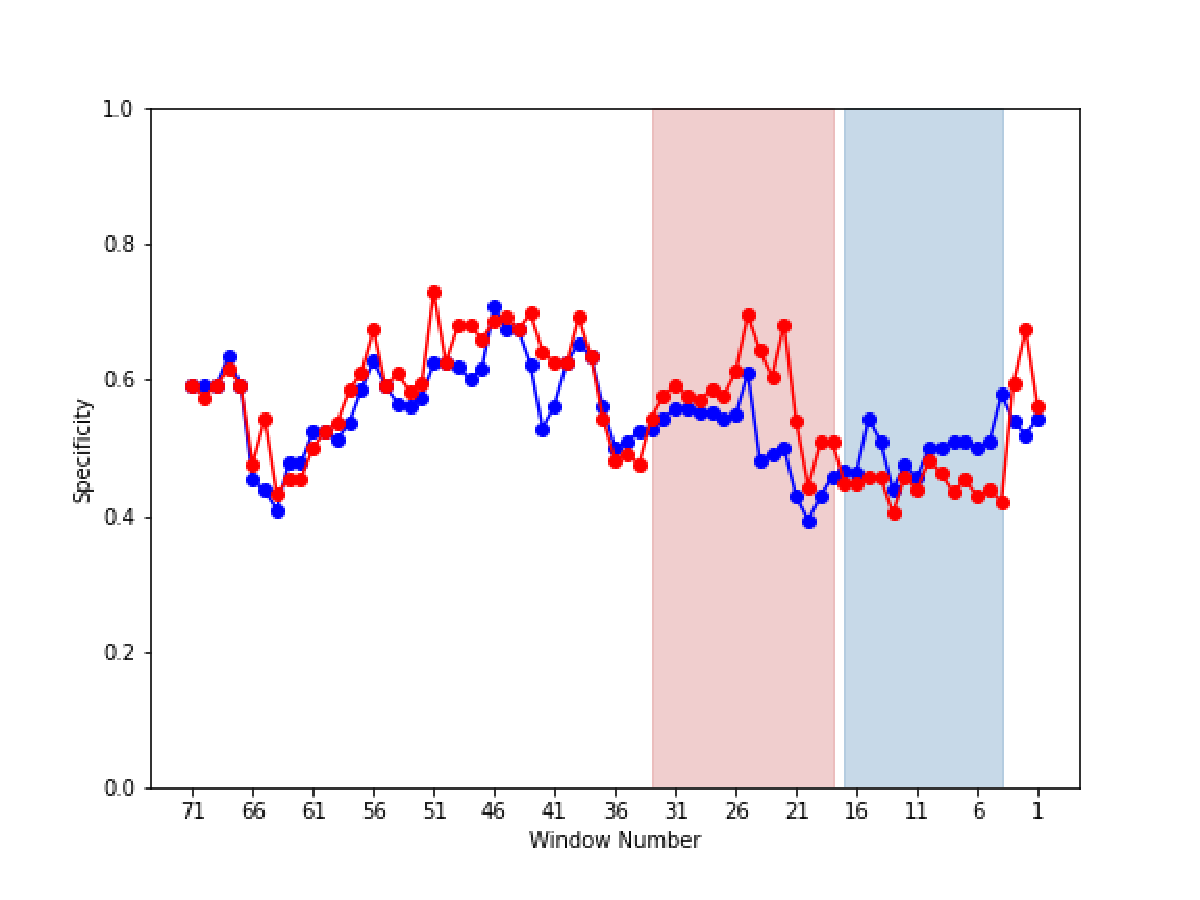
\includegraphics[width=0.495\textwidth]{Uenaka_fig/RQ2_result/Neutron_review_Specificity.pdf}
    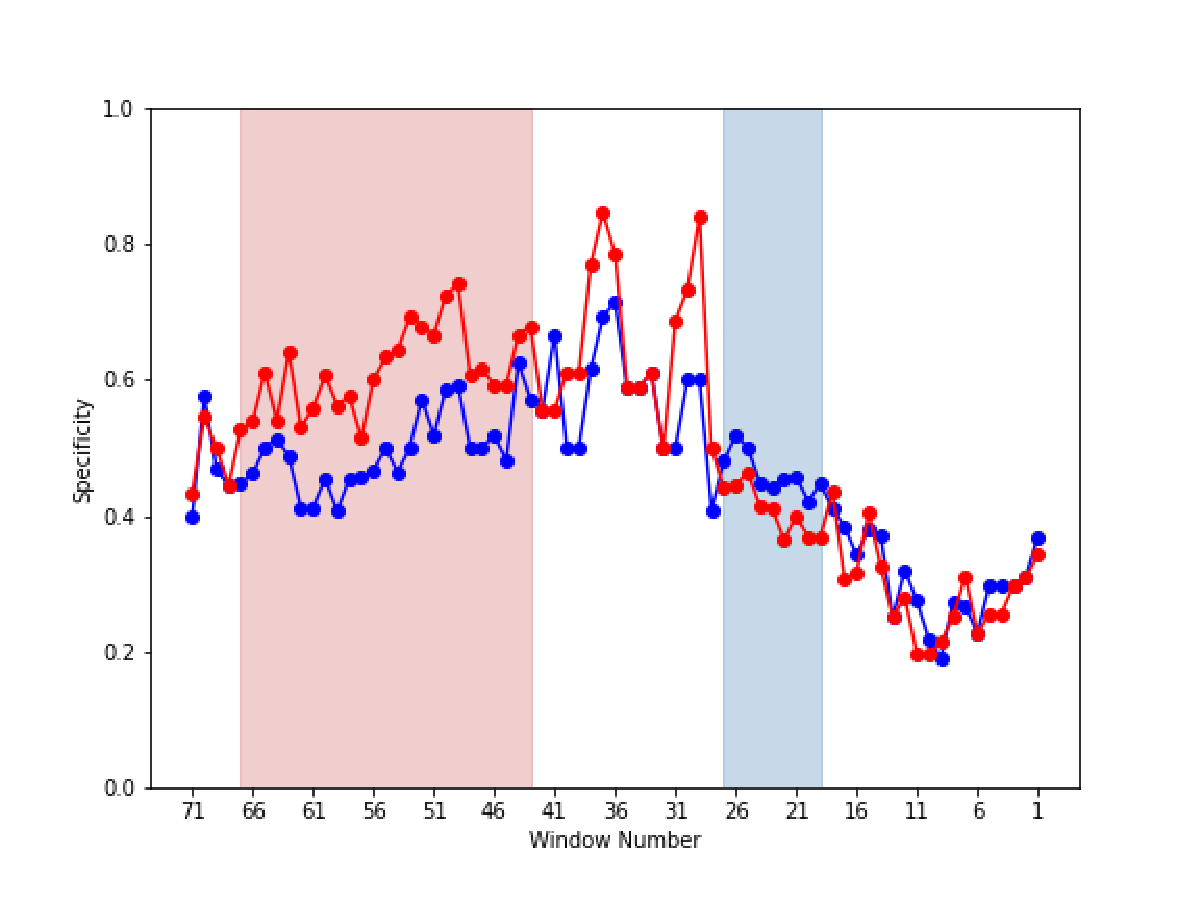
\includegraphics[width=0.495\textwidth]{Uenaka_fig/RQ2_result/Cinder_review_Specificity.pdf}
    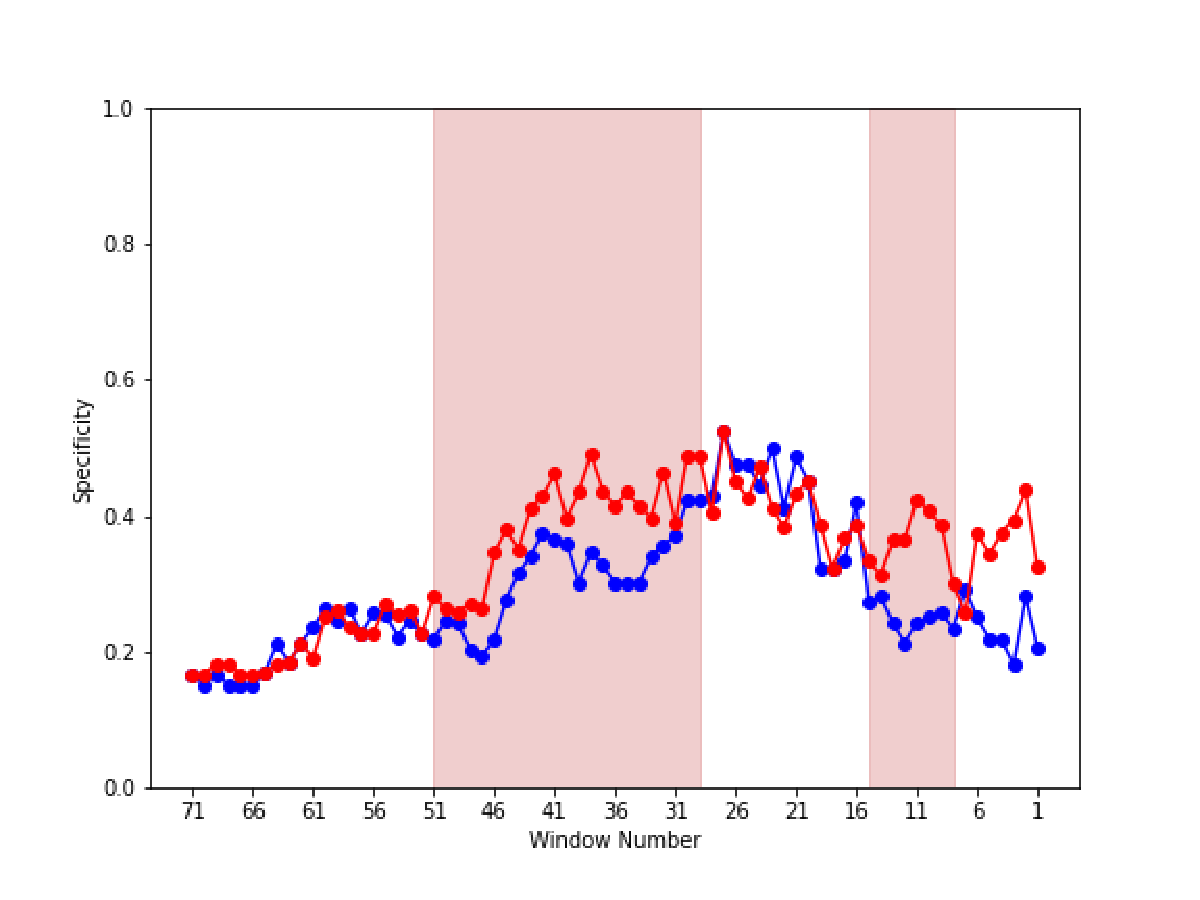
\includegraphics[width=0.495\textwidth]{Uenaka_fig/RQ2_result/Keystone_review_Specificity.pdf}
    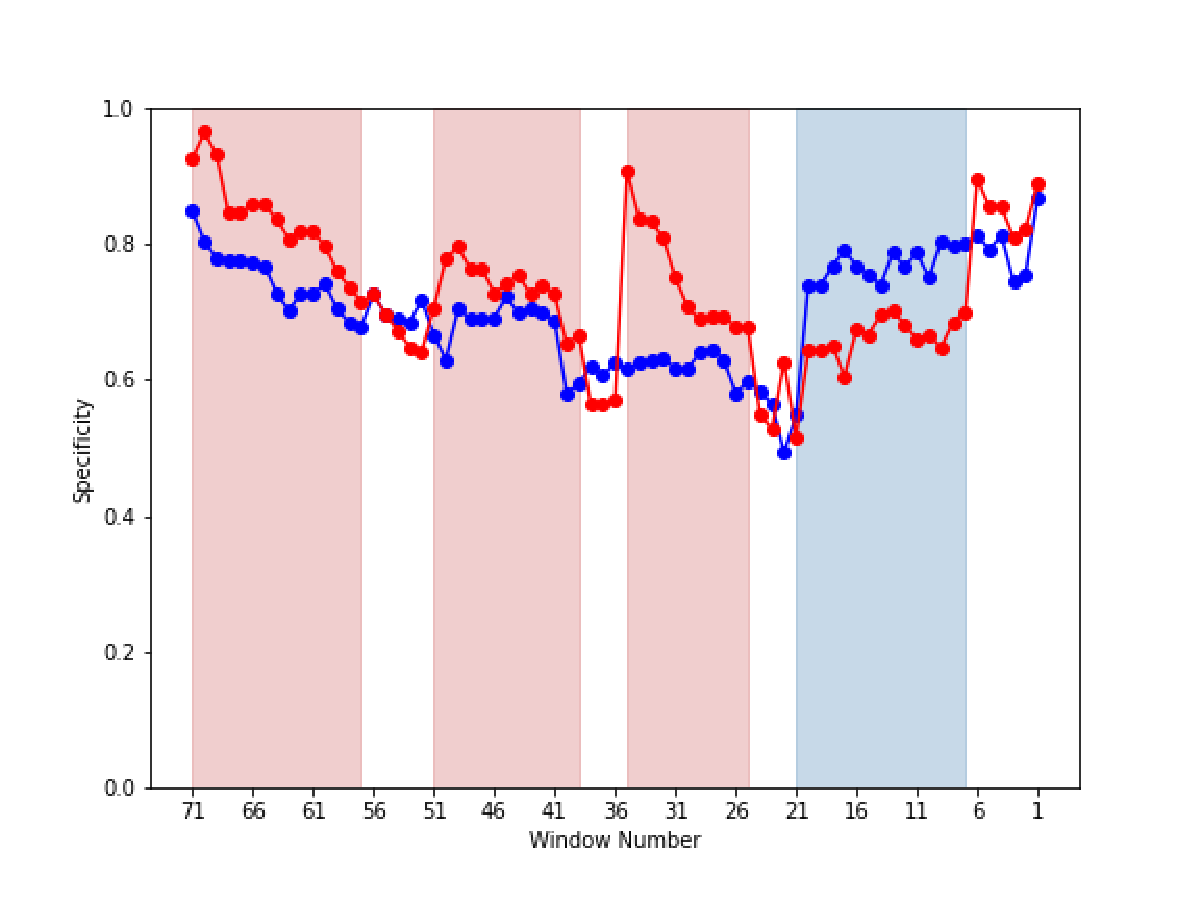
\includegraphics[width=0.495\textwidth]{Uenaka_fig/RQ2_result/Swift_review_Specificity.pdf}
    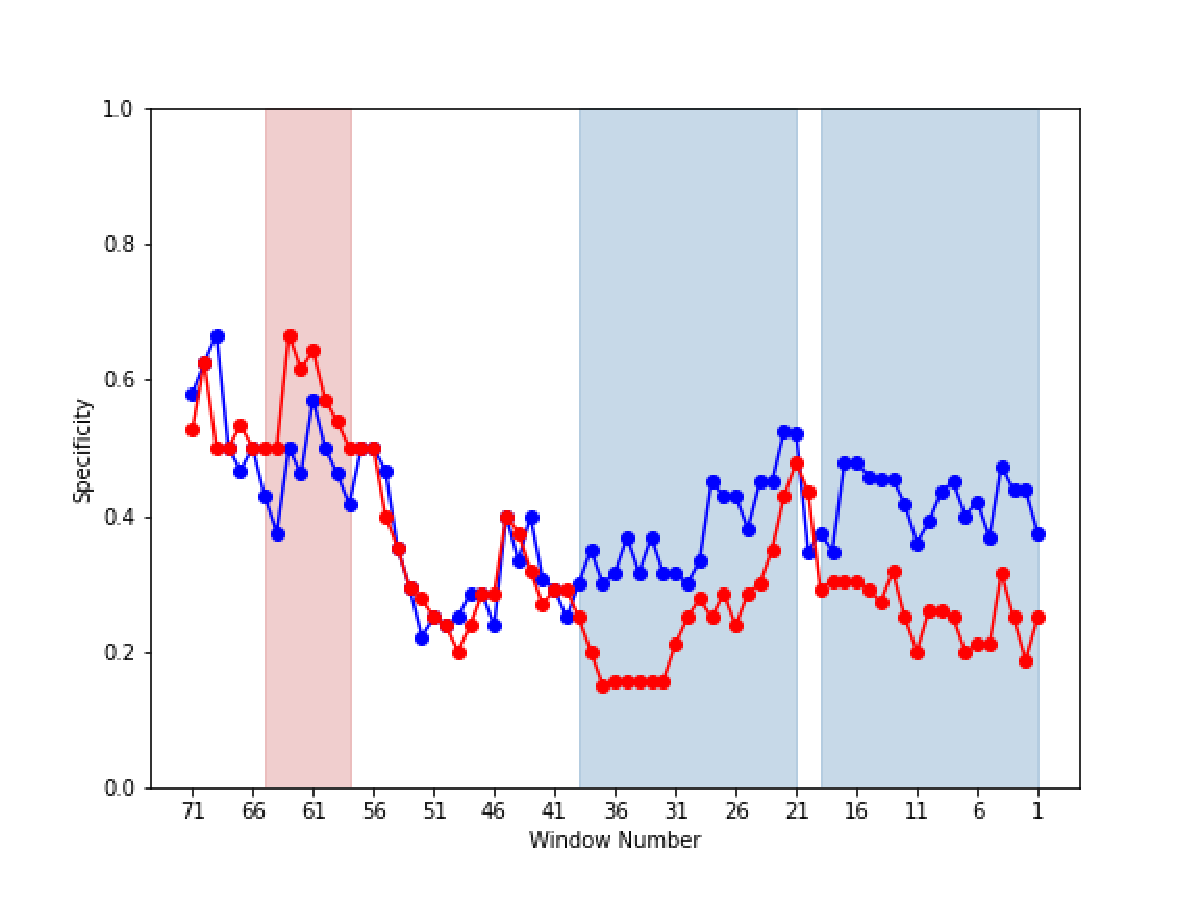
\includegraphics[width=0.495\textwidth]{Uenaka_fig/RQ2_result/Glance_review_Specificity.pdf}
    \caption{検証予測モデルの特異度(上段左:Nova,上段右:Neutron,中段左:Cinder,\\ 中段右:Keystone,下段左:Swift,下段右:Glance)(赤:提案モデル,青:ベースラインモデル)}
    \label{fig:review_spec}
\end{center}
\end{figure}
%-----------------------


\subsection{導入予測モデル}
導入予測モデルの予測結果として,図\ref{fig:merge_spec}は各プロジェクトの特異度を示す.図は縦軸が特異度を表し,横軸や折れ線,図の配置や色で表されている期間の定義は\ref{sec:rq1_kenshou}項と同様である.特異度および再現率についてまとめたものを図\ref{fig:merge_sperec_window}に示す.また,表\ref{table:merge_spec_jikeiretsu}はベースラインモデルの再現率および特異度の時系列変化の分析結果として,各プロジェクトの導入予測モデルにおける再現率および特異度の回帰係数の分類を示す.表\ref{table:merge_spec_jikeiretsu}において,回帰係数の分類は表\ref{table:review_seino_jikeiretsu}と同様の矢印で表す.

\subsubsection{知見3:4プロジェクト (Neutron, Cinder, Keystone, Glance) ではリリースが近づくにつれてチケットおよびチケット実装者の特徴に基づいて導入しないチケットを判断するようになり,2プロジェクト (Nova, Swift) では判断の割合が変化しない}
本知見では,知見1と同様に各プロジェクトでチケットおよびチケット実装者の特徴から,チケットに対する導入判断を正しく判別できるチケットの割合がリリースまでの期間内でどのように変化するかを明らかにする.表\ref{table:merge_seino_jikeiretsu}の回帰係数の分類から,ベースラインモデルの特異度は4プロジェクト (Neutron, Cinder, Keystone, Glance) において回帰係数が有意に増加し,2プロジェクト (Nova, Swift) において回帰係数が有意に増加および減少しないという結果が得られた.また,ベースラインモデルの再現率は2プロジェクト (Neutron, Cinder) において回帰係数が有意に増加し,2プロジェクト (Keystone, Swift) において回帰係数が有意に減少し,2プロジェクト (Nova, Glance) において回帰係数が有意に増加および減少しないという結果が得られた.以下に共通の傾向を持つプロジェクトの結果をまとめる.

\textbf{ (Neutron, Cinder, Keystone, Glance) }リリースが近づくにつれて,チケットおよびチケット実装者の特徴から正しく負例と判別できるチケットの割合が増加し,正しく正例と判別できるチケットの割合は増加する (Neutron, Cinder) ,減少する (Keystone) リリース期間全体を通して概ね一定である (Glance) ことを明らかにした.この結果から,当該プロジェクトの検証者はリリースが近づくにつれて,チケットおよびチケット実装者の特徴に基づいて導入しないチケットを判断するようになることが示唆される.

\textbf{ (Nova, Swift) }リリース期間全体を通して,チケットおよびチケット実装者の特徴から正しく負例と判別できるチケットの割合が概ね一定であり,リリースが近づくにつれて,正しく正例と判別できるチケットの割合は減少する (Nova) ,リリース期間全体を通して概ね一定である (Swift) ことを明らかにした.この結果から,当該プロジェクトの検証者はリリース期間全体を通して,チケットおよびチケット実装者の特徴に基づいて導入しないチケットを判断する割合が変化しないことが示唆される.

%--------------------
\begin{table*}[t]
\caption{各プロジェクトの導入予測モデルにおける再現率(再掲),特異度の回帰係数の分類}
\label{table:merge_spec_jikeiretsu}
\centering
\vspace{0.5zh}
\scalebox{0.9}{
\begin{tabular}{l|c|c|c|c|c|c}
    \hline \hline
    評価指標 & Nova & Neutron & Cinder & Keystone & Swift & Glance \\ \hline
    再現率 & $\rightarrow$ & $\nearrow$ & $\nearrow$ & $\searrow$ & $\searrow$ & $\rightarrow$ \\ \hline
    特異度 & $\rightarrow$ & $\nearrow$ & $\nearrow$ & $\nearrow$ & $\rightarrow$ & $\nearrow$ \\ \hline
\end{tabular}}
\end{table*}
%--------------------


\subsubsection{知見4:開発状況によって検証者の導入判断が一部のチケットで変化する期間および判断の変化はプロジェクトによって異なり,Glance以外の全てのプロジェクトで後期の一部のチケットは,開発状況によって検証者が導入するようになる}
本知見では,リリース期間を前期(リリースが遠い時)・中期(リリース中頃)・後期(リリースが近い時)の3つに分割し,開発状況によって検証者の導入判断が一部のチケットで変化する期間および判断の変化を明らかにする.図\ref{fig:merge_sperec_window}の結果から,\ref{sec:ticket_tokutei}節の解釈に従ってプロジェクトごとの傾向をまとめる.

\textbf{ (Nova) }前期の一部のチケットは,開発状況によって検証者が導入しないようになり,中期および後期の一部のチケットは,開発状況によって検証者が導入するようになることが示唆される.

\textbf{ (Neutron) }前期の一部のチケットは,開発状況によって検証者が導入するもしくは導入しないようになり,中期の一部のチケットは,開発状況によって検証者が導入しないようになることが示唆される.

\textbf{ (Cinder) }前期および中期の一部のチケットは,開発状況によって検証者が導入しないようになり,後期の一部のチケットは,開発状況によって検証者が導入するようになることが示唆される.

\textbf{ (Keystone) }前期の一部のチケットは,開発状況によって検証者が導入しないようになり,中期および後期の一部のチケットは,開発状況によって検証者が導入するようになることが示唆される.

\textbf{ (Swift) }前期や中期の一部のチケットは,開発状況によって検証者が導入しないようになり,後期の一部のチケットは,開発状況によって検証者が導入するようになることが示唆される.

\textbf{ (Glance) }前期や中期の一部のチケットは,開発状況によって検証者が導入しないようになることが示唆される.


%-----------------------
\begin{figure}[t]
\begin{center}
    \includegraphics[width=1.0\textwidth]{Uenaka_fig/RQ2_result/merge_sperec_window.pdf}
    \caption{導入予測モデルの予測結果:7つ以上の連続したウィンドウにおいて提案モデルの特異度,再現率がベースラインモデルの特異度,再現率と比べて向上した期間}
    \label{fig:merge_sperec_window}
\end{center}
\end{figure}
%-----------------------

%-----------------------
\begin{figure}[H]
\begin{minipage}{\textwidth}
\vspace{0.08\textheight}
\begin{center}
    \includegraphics[width=0.495\textwidth]{Uenaka_fig/RQ2_result/Nova_merge_Specificity.pdf}
    \includegraphics[width=0.495\textwidth]{Uenaka_fig/RQ2_result/Neutron_merge_Specificity.pdf}
    \includegraphics[width=0.495\textwidth]{Uenaka_fig/RQ2_result/Cinder_merge_Specificity.pdf}
    \includegraphics[width=0.495\textwidth]{Uenaka_fig/RQ2_result/Keystone_merge_Specificity.pdf}
    \includegraphics[width=0.495\textwidth]{Uenaka_fig/RQ2_result/Swift_merge_Specificity.pdf}
    \includegraphics[width=0.495\textwidth]{Uenaka_fig/RQ2_result/Glance_merge_Specificity.pdf}
    \caption{導入予測モデルの特異度(上段左:Nova,上段右:Neutron,中段左:Cinder,\\ 中段右:Keystone,下段左:Swift,下段右:Glance)(赤:提案モデル,青:ベースラインモデル)}
    \label{fig:merge_spec}
\end{center}
\vspace{0.08\textheight}
\end{minipage}
\end{figure}
%-----------------------

% \section{チケットの特定結果}\label{sec:ticket_tokutei_result}
% \subsection{リリース期間全体を通して常に優先されるチケット}

% \subsection{リリース期間全体を通して常に優先されないチケット}

% \subsection{リリースまでの期間内で優先度が変化するチケット}

%%%%%%%%%%%%%%%%%%%%%%
\chapter{妥当性の脅威}\label{sec:disc}
%%%%%%%%%%%%%%%%%%%%%%

\section{内的妥当性}
本研究で取り扱う検証予測モデルでは,ウィンドウ内の2週間より前に検証が開始されたチケットは既に優先されたチケットとみなし分析対象外としている.しかし,実装者が検証者からの修正要求に基づき改修したソースコードを再報告した場合,検証者は検証が開始されていないチケットだけでなく再報告されたチケットも含めて,優先して検証するチケットを選択していることが示唆される.ただし,本研究では,検証が開始されていないチケットの中で,優先的に検証されるチケットがリリースまでの期間によってどのように変化するのかに焦点を当てている.そのため,再報告されたチケットが分析結果のノイズとなることを防ぐことで,検証が開始されていないチケットについての十分な知見を得ることができたと考える.

本研究では,従来研究\cite{prioritizer}で提案されているチケットおよびチケット実装者の特徴(7種類)と従来研究\cite{release_merge}\cite{review1}の知見から有用と示唆される実装者や変更内容の特徴(5種類)を説明変数に用いてベースラインモデルを構築したため,チケットのソースコード変更に関する特徴量(例えば,複雑度)など,より詳細なソースコードレベルの特徴量を説明変数に用いることで予測性能が向上することが示唆される.ただし,本研究でデータセットとして用いたOpenStackプロジェクトのコアコンポーネント6プロジェクトが利用するGerritでは,コードレビューチケットのリストを閲覧できる機能が提供されている.本研究では主に上記のリストから取得可能な情報をもとに特徴量を収集することで,脅威を削減する.

\section{外的妥当性}
本研究では,ケーススタディとしてOpenStackプロジェクトのコアコンポーネント6プロジェクトのコードレビューチケットを対象とした.対象とするプロジェクトやリリースバージョンを変更した場合に分析結果および予測精度が変化することが示唆される.しかし,本研究ではGerritを利用するプロジェクトの中でもコードレビューチケットが多く提案されているOpenStackプロジェクトのコアコンポーネントプロジェクトを対象としている.また,その中でも導入されたチケットの多いバージョンを対象とすることで,脅威を削減する.
%している.そのため,データセットとするプロジェクトやリリースバージョンの変更による分析結果および予測精度への影響は低いと示唆する.

%%%%%%%%%%%%%%%%%%%%%%
\chapter{おわりに}\label{sec:fig-tab-exp}
%%%%%%%%%%%%%%%%%%%%%%
hoge
% 本論文では,リリースまでの期間に応じて優先的に検証/導入されるコードレビューチケットの予測を目的に,2つのRQを検証した.データセットとして,OpenStackプロジェクトのコアコンポーネント6プロジェクト(Nova,Neutron,Cinder,Keystone,Swift,Glance)を分析対象とし,チケットの特徴量を収集,比較することで,リリースまでの期間に応じて優先的に検証/導入されるチケットの特徴が異なることを明らかにした.また,それらの特徴量を学習させることで,直近のバージョンリリースに向けて検証される変更提案や導入される変更提案の予測モデルを構築した.モデルの予測精度を評価した結果,提案手法とベースライン手法の精度に大きな差は見られなかった.
% また,考察した結果から提案手法は負例(優先的に検証/導入する必要のないチケット)を正確に検出できることが明らかとなった.今後は,優先的に検証,または導入するチケットの特徴が変わる時点を見積もる手法を確立する.

%%%%%%%%%%%%%%%%%%%%%%%%%%%%%%%%%%%%%%%%%%%%%%%%%%%%%%%%%%%%%%%%%%%%%%%%

%%
%% 謝辞
%%
%% \begin{acknowledgements}
%% 感謝します.
%% \end{acknowledgements}

%%%%%%%%%%%%%%%%%%%%%%%%%%%%%%%%%%%%%%%%%%%%%%%%%%%%%%%%%%%%%%%%%%%%%%%%

%%
%% 参考文献
%%
\bibliographystyle{junsrt}
\bibliography{@MSthesis2024_Uenaka/Uenaka_thesis}



%%%%%%%%%%%%%%%%%%%%%%%%%%%%%%%%%%%%%%%%%%%%%%%%%%%%%%%%%%%%%%%%%%%%%%%%

%%
%% 付録
%%
% \appendix
% 
% \chapter{サンプルプログラム}
% 
% プログラムリストや実行結果など,本論を補足する上で必要と思われるものが
% あれば付録として付ける.
% 
% {
% \footnotesize
% \begin{verbatim}
% #include <stdio.h>
% int main(void)
% {
%     printf("Hello, World!\n");
%     return 0;
% }
% \end{verbatim}
% }

%%%%%%%%%%%%%%%%%%%%%%%%%%%%%%%%%%%%%%%%%%%%%%%%%%%%%%%%%%%%%%%%%%%%%%%%

\end{document}
